 %%%%%%%%%%%%%%%%%%%%%%%%%%%%%%%%%%%%%%%%%%%%%%%%%%%%%%%%%
 %
 %	Name			:: 	The official template for the typesetting of diploma theses at the Faculty of Computer Science of AGH University of Krakow
 %	Author			:: 	Stanisław Polak (polak[aT]icsr[DoT]agh[DoT]edu[DoT]pl)
 %	Created			::	2024-02-14
 %	Modified	    ::	2024-06-13
 %	Version			:: 	1.3.2
 %	Email			:: 	polak[aT]icsr[DoT]agh[DoT]edu[DoT]pl
 %	Website			:: 	http://www.icsr.agh.edu.pl/~polak/
 %   Youtube         ::  https://www.youtube.com/user/spolak69
 %   Github          ::  https://github.com/polaksta
 %	License			:: 	This work may be distributed and/or modified under the
 %                       conditions of the LaTeX Project Public License, either version 1.3
 %                       of this license or (at your option) any later version.
 %                       The latest version of this license is in
 %                       http://www.latex-project.org/lppl.txt
 %                       and version 1.3 or later is part of all distributions of LaTeX
 %                       version 2005/12/01 or later.
 %
 %	Description		::	This document is a demonstration of the template
 %
 %%%%%%%%%%%%%%%%%%%%%%%%%%%%%%%%%%%%%%%%%%%%%%%%%%%%%%%%%
 % Niniejszy dokument — szkielet pracy dyplomowej — prezentuje przykłady użycia klasy 'agh-wi' oraz pakietów tradycyjnie używanych w pracach
 % dyplomowych z informatyki. Dla kilku z nich, wartości początkowe parametrów konfiguracyjnych są zdefiniowane 
 % w klasie  — wartości te uwzględniają uwagi osób prowadzących przedmiot "Pracownia Dyplomowa". 
 % Oczywiście możesz używać dowolnych pakietów, niekoniecznie tych, które są pokazane w tym dokumencie
 %%%%%%%%%%%%%%%%%%%%%%%%%%%%%%%%%%%%%%%%%%%%%%%%%%%%%%%%%
 % Poniższe uwagi NIE DOTYCZĄ Overleaf-a
 %%%%%%%%%%%%%%%%%%%%%%%%%%%%%%%%%%%%%%%%%%%%%%%%%%%%%%%%%
 % W tej przykładowej pracy dyplomowej użyto, między innymi, pakietów:
 %   - "minted", co oznacza, że musisz uruchomić kompilator z opcją '-shell-escape'
 %   - "biblatex", co oznacza, że po kompilacji (dokumentu) musisz, jeszcze, wygenerować plik '.bbl'
 %   - "nomencl", co oznacza, że za pomocą komendy 'makeindex' musisz wygenerować wykaz symboli
 %
 % Tak więc, w celu wygenerowania wynikowego dokumentu PDF, musisz wykonać następujące komendy:
 %       pdflatex -shell-escape example
 %       biber example
 %       makeindex example.nlo  -s nomencl.ist -o example.nls
 %       pdflatex -shell-escape example
 %       pdflatex -shell-escape example
 %
 % Dodatkowo musisz mieć zainstalowany program 'pygmentize', który jest częścią pakietu "Pygments" (https://pygments.org/)
 % Ww. programy powinny zainstalować się automatycznie podczas instalacji pakietów LaTeX
 %
 % Jeżeli masz zainstalowany program 'latexmk', to możesz wygenerować dokument PDF następująco:
 %       latexmk example
 %       makeindex example.nlo  -s nomencl.ist -o example.nls
 %       latexmk example
 %
 % Do edycji (oraz komplilacji) dokumentów LaTeX polecam program 'TeXstudio' (https://www.texstudio.org/)
 %
 % Autor: Stanisław Polak <polak[aT]agh[DoT]edu[DoT]pl>
 %%%%%%%%%%%%%%%%%%%%%%%%%%%%%%%%%%%%%%%%%%%%%%%%%%%%%%%%%
% \documentclass{agh-wi} % Praca po polsku; na stronie tytułowej, najpierw jest widoczny polskojęzyczny tytuł, a potem angielskojęzyczny.
                       % Kierunek 'Informatyka'.
                       % Przeznaczona do oglądania przy użyciu przeglądarki PDF.
 %%%%%%%%%%%%%%%%%%%%%%%%%%%%%%%%%
 % Inne, przykładowe, użycia klasy
 %%%%%%%%%%%%%%%%%%%%%%%%%%%%%%%%%
 \documentclass[english]{agh-wi}     % Praca po angielsku; 
                                       %     strona tytułowa po polsku, ale najpierw jest widoczny angielskojęzyczny tytuł, a potem polskojęzyczny.  
                                       % Kierunek 'Informatyka'.
                                       % Przeznaczona do oglądania przy użyciu przeglądarki PDF.
 % \documentclass[english, ds]{agh-wi} % Praca po angielsku; ...
                                       % Kierunek 'Informatyka - Data Science'.
                                       % Przeznaczona do oglądania przy użyciu przeglądarki PDF.
 % \documentclass[umisi]{agh-wi}       % Praca po polsku; ...
                                       % Kierunek 'Informatyka - Uczenie Maszynowe i Sztuczna Inteligencja'.
                                       % Przeznaczona do oglądania przy użyciu przeglądarki PDF.
 % \documentclass[print]{agh-wi}       % Praca po polsku; ...
                                       % Kierunek 'Informatyka'.
                                       % Przeznaczona do drukowania - każda strona posiada,
                                       %    dodatkowy (2cm), margines na oprawę.
 %%%%%%%%%%%%%%%%%%%%%%%%%%%%%%%%%%%%%
 % Parametry dla strony tytułowej
 %%%%%%%%%%%%%%%%%%%%%%%%%%%%%%%%%%%%%
\titlePL{Automatyczna klasyfikacja choroby Chagasa na podstawie sygnałów elektrokardiograficznych }  % Tytuł po polsku
\titleEN{Automatic classification of Chagas disease based on electrocardiogram signals} % Tytuł po angielsku
\author{Juliusz Antoni Wasieleski}
\supervisor{dr. inż. Szymon Sieciński}
 %%%%%%%%%%%%%%%%%%%%%%%%%%%%%%%%%%%%%
 % Pakiety
 %%%%%%%%%%%%%%%%%%%%%%%%%%%%%%%%%%%%%
 % Podstawowe — na pewno będziesz ich potrzebował(a) w swojej wersji pracy dyplomowej
 %%%%%%%%%%%%%%%%%%%%%%%%%%%%%%%%%%%%%
\usepackage{polski} % Obsługa języka polskiego
 %%%%%%%%%%%%%%%%%%%%%%%%%%%%%%%%%%%%%
 % Dodatkowe — niekoniecznie będziesz ich potrzebował(a) w swojej wersji pracy dyplomowej
 %%%%%%%%%%%%%%%%%%%%%%%%%%%%%%%%%%%%%
\usepackage[sorting=none]{biblatex}           % Spis literatury ma być tworzony na podstawie zawartości bibliograficznej bazy danych
\usepackage{amsmath}                          % Dodatkowe środowiska matematyczne
\usepackage{amssymb}                          % Dodatkowe symbole matematyczne
\usepackage[polish, intoc]{nomencl}           % Definiowanie symboli
\usepackage{graphicx}                         % Wstawianie grafik zewnętrznych
\usepackage{xcolor}                           % Kolorowy tekst
\usepackage{tabularx}                         % Rozszerzona wersja środowiska 'tabular'
\usepackage{longtable}                        % Skład "długich" tabel
\usepackage[ruled,linesnumbered]{algorithm2e} % Algorytmy w formie pseudokodu
\usepackage{listings}                         % Formatowanie kodów źródłowych programów
\usepackage[newfloat]{minted}                 % Formatowanie kodów źródłowych programów
\usepackage{hyperref}                         % Obsługa adresów URL — zbędny jeżeli używasz 'biblatex'
\usepackage{csquotes}                         % Polskie cudzysłowy — rekomendowany jeżeli używasz 'biblatex'
 %%%%%%%%%%%%%%%%%%%%%%%%%%%%%%%%%%%%
 %  % Konfiguracja rysunków TikZ
 %%%%%%%%%%%%%%%%%%%%%%%%%%%%%%%%%%%%
\usetikzlibrary{shapes.geometric,arrows.meta,positioning,calc}
\tikzstyle{every picture}+=[remember picture]
\tikzstyle{na} = [baseline=-.5ex]
 %%%%%%%%%%%%%%%%%%%%%%%%%%%%%%%%%%%%
 % Ładowanie danych bibliograficznych
 %%%%%%%%%%%%%%%%%%%%%%%%%%%%%%%%%%%%
\addbibresource{bibliography.bib}
 %%%%%%%%%%%%%%%%%%%%%%%%%%%%%%%%%%%%%
 % Opcje konfiguracyjne pakietów
 %%%%%%%%%%%%%%%%%%%%%%%%%%%%%%%%%%%%%
 % Pakiet 'framed'
\definecolor{shadecolor}{gray}{0.9}
 % Pakiet 'nomencl'
\makenomenclature % Otwórz plik 'example.nlo'
 %%%%%%%%%%%%%%%%%%%%%%%%%%%%%%%%%%%%%
 % Definicje komend
 %%%%%%%%%%%%%%%%%%%%%%%%%%%%%%%%%%%%%
\newcommand{\alert}[1]{\colorbox{red!50}{#1}}
 %%%%%%%%%%%%%%%%%%%%%%%%%%%%%%%%%%%%%
 % Twierdzenia i podobne struktury
 %%%%%%%%%%%%%%%%%%%%%%%%%%%%%%%%%%%%%
\newtheorem{theorem}{Twierdzenie}
\newtheorem{definition}{Definicja}

\newcounter{comment}[chapter]
\newenvironment{comment}[1][]{\begin{shaded}\refstepcounter{comment}
   \noindent \textbf{Uwaga~\thechapter.\thecomment. #1} \rmfamily}{\end{shaded}}
 %%%%%%%%%%%%%%%%%%%%%%%%%%%%%%%%%%%%%
 % Treść poszczególnych rozdziałów tej, przykładowej, pracy dyplomowej 
 %   znajduje się w osobnych plikach (patrz  katalog 'tex') 
 %   i jest dołączana, do bieżącego pliku, komendą \include. 
 % Tworząc pracę, z reguły, zajmujesz się edycją 
 %   tylko jednego rozdziału. 
 % Aby skrócić czas kompilacji warto, za pomocą komendy \includeonly, 
 %   włączyć kompilację tylko tego pliku (rozdziału) nad którym, aktualnie, pracujesz
 %%%%%%%%%%%%%%%%%%%%%%%%%%%%%%%%%%%%%
 % \includeonly{tex/example,tex/notes} % Kompiluj, tylko, treść wymienionych plików, tj. 'tex/example.tex' oraz 'tex/notes.tex'.
 %%%%%%%%%%%%%%%%%%%%%%%%%%%%%%%%%%%%%
 %%%%%%%%%%%%%%%%%%%%%%%%%%%%%%%%%%%%%
\begin{document}
 %%%%%%%%%%%%%%%%%%%%%%%%%%%%%%%%%%%%%
\frontmatter % Część wstępna
 %%%%%%%%%%%%%%%%%%%%%%%%%%%%%%%%%%%%%
\maketitle % Dodaj stronę tytułową
 %%%%%%%%%%%%%%%%%%%%%%%
 % Jeżeli chcesz komuś podziękować, to możesz użyć poniższego kodu
% \cleardoublepage
% \thispagestyle{empty}
% \vspace*{\fill}
% \begin{flushright}
%     \em
%     \begin{minipage}{0.75\textwidth}
%         Tutaj możesz umieścić treść podziękowań.
%         Tutaj możesz umieścić treść podziękowań.
%         Tutaj możesz umieścić treść podziękowań.
%         Tutaj możesz umieścić treść podziękowań.
%         Tutaj możesz umieścić treść podziękowań.
%     \end{minipage}
% \end{flushright}
 %%%%%%%%%%%%%%%%%%%%%%%
\begin{abstractPL}
    Choroba Chagasa, wywoływana przez pasożyta Trypanosoma cruzi, stanowi poważny problem zdrowotny w Ameryce Łacińskiej i jest coraz częściej rozpoznawana w innych regionach ze względu na migrację. Zajęcie serca, które można wykryć na podstawie nieprawidłowości w elektrokardiogramie (EKG), jest jednym z najpoważniejszych powikłań, jednak jego wczesna identyfikacja pozostaje trudna. Celem niniejszej pracy jest rozwiązanie tego problemu poprzez dostarczenie narzędzia obliczeniowego do automatycznego wykrywania zmian związanych z chorobą Chagasa w sygnałach EKG.

W pracy zbadano systematyczny program szesnastu podejść do automatycznego wykrywania choroby Chagasa, ocenianych na zbiorach danych CODE-15\% oraz SaMi-Trop z konkursu „Detection of Chagas Disease from the ECG: The George B. Moody PhysioNet Challenge 2025”. Badane podejścia obejmują bazowe klasyfikatory 1-D ResNet, generatywną augmentację danych za pomocą modeli dyfuzyjnych, sieci neuronowe informowane fizyką oparte na modelach Alieva-Panfilova i McSharry'ego oraz samonadzorowane modele fundamentalne EKG. Wszystkie eksperymenty przeprowadzono na sprzęcie konsumenckim Apple M3, co czyni pracę studium przypadku w nurcie Green AI.
Najlepszy model dyfuzyjny informowany fizyką osiągnął wynik Challenge Score (czułość przy 5\% odsetku fałszywie dodatnich) równy 0,2289, natomiast dostrojony model samonadzorowany uzyskał najwyższe AUROC w rozkładzie zgodnym z treningiem, równe 0,8593. Wyniki rozchodzą się przy generalizacji: model o najwyższym AUROC całkowicie zawiódł na kohorcie SaMi-Trop spoza rozkładu treningowego (czułość 0,0000), podczas gdy autoenkoder fenomenologiczny o niższym AUROC odzyskał 99,45\% tej kohorty po jednej korekcie progu decyzyjnego. AUROC błędnie szereguje zatem modele dla klinicznego zadania przesiewowego, a kryteria oceny powinny być dostosowane do warunków spoza rozkładu treningowego.
\end{abstractPL}
\begin{abstractEN}
    Chagas disease, caused by the parasite Trypanosoma cruzi, is a major health concern in Latin America and is increasingly recognized in other regions due to migration. Cardiac involvement, which can be detected through electrocardiogram (ECG) abnormalities, is one of the most serious complications, yet its early identification remains challenging. The aim of this thesis is to address this issue by providing a computational tool for the automatic detection of Chagas-related changes in ECG signals.

This thesis investigates a systematic program of sixteen approaches to automated Chagas detection, evaluated on the CODE-15\% and SaMi-Trop datasets of the "Detection of Chagas Disease from the ECG: The George B. Moody PhysioNet Challenge 2025". The approaches span baseline 1-D ResNet classifiers, generative data augmentation with diffusion models, physics-informed neural networks based on the Aliev-Panfilov and McSharry models, and self-supervised ECG foundation models. All experiments were conducted on consumer-grade Apple M3 hardware, framing the work as a Green-AI case study.
The strongest physics-guided diffusion model reached a Challenge Score (true positive rate at 5\% false positive rate) of 0.2289, while a fine-tuned self-supervised model achieved the highest in-distribution AUROC of 0.8593. The two rankings diverge under generalization: the model with the highest AUROC failed entirely on the out-of-distribution SaMi-Trop cohort (0.0000 sensitivity), whereas a lower-AUROC phenomenological autoencoder recovered 99.45\% of that cohort after a single decision-threshold adjustment. AUROC therefore misranks models for the clinical screening task, and evaluation criteria should be aligned with out-of-distribution deployment.
\end{abstractEN}
 %%%%%%%%%%%%%%%%%%%%%%%%%%%%%%%%%%%%%
 % AI-tool usage declaration
 %%%%%%%%%%%%%%%%%%%%%%%%%%%%%%%%%%%%%
\cleardoublepage
\thispagestyle{empty}
\vspace*{\fill}
\begin{center}
\begin{minipage}{0.8\textwidth}
\begin{center}\textbf{Declaration on the use of AI tools}\end{center}
\noindent In the preparation of the text of this master's thesis, AI-powered linguistic tools were used to improve the clarity and coherence of the manuscript and ensure its stylistic and grammatical correctness.

\medskip
\noindent However, the content, ideas, research findings, and conclusions presented herein are solely the author's own.
\end{minipage}
\end{center}
\vspace*{\fill}
\cleardoublepage
 %%%%%%%%%%%%%%%%%%%%%%%%%%%%%%%%%%%%%
 %%%%%%%%%%%%%%%%%%%%%%%%%%%%%%%%%%%%%
\tableofcontents   % Wygeneruj spis treści
\listoffigures     % Wygeneruj listę rysunków
\listoftables      % Wygeneruj listę tabel
\cleardoublepage
\phantomsection
\addcontentsline{toc}{chapter}{List of Abbreviations}
\chapter*{List of Abbreviations}

\begingroup
\renewcommand{\arraystretch}{1.25}
\begin{longtable}{@{}p{2.4cm}@{\hspace{1em}}p{\dimexpr\textwidth-3.4cm\relax}@{}}
AdaGN     & Adaptive Group Normalization \\
AdamW     & Adam optimizer with decoupled weight decay \\
AdapRes   & Adaptive Residual Block \\
AF        & Atrial Fibrillation \\
AGH       & AGH University of Krakow \\
AI        & Artificial Intelligence \\
AP        & Aliev--Panfilov (model) \\
AUPRC     & Area Under the Precision--Recall Curve \\
AUROC     & Area Under the Receiver Operating Characteristic Curve \\
CI        & Confidence Interval \\
CNN       & Convolutional Neural Network \\
CODE-15\% & Clinical Outcomes in Digital Electrocardiography (15\% subset) \\
CPU       & Central Processing Unit \\
DDPM      & Denoising Diffusion Probabilistic Model \\
ECG       & Electrocardiogram \\
EMA       & Exponential Moving Average \\
EP        & Electrophysiology / Electrophysiological \\
FN        & False Negative \\
FP        & False Positive \\
FPR       & False Positive Rate \\
GAP       & Global Average Pooling \\
GELU      & Gaussian Error Linear Unit \\
GPU       & Graphics Processing Unit \\
ID        & In-Distribution \\
LAFB      & Left Anterior Fascicular Block \\
LDM       & Latent Diffusion Model \\
LN        & Layer Normalization \\
LR        & Learning Rate \\
LVH       & Left Ventricular Hypertrophy \\
MLP       & Multilayer Perceptron \\
MPS       & Metal Performance Shaders (Apple) \\
MSE       & Mean Squared Error \\
OOD       & Out-of-Distribution \\
PCA       & Principal Component Analysis \\
PDE       & Partial Differential Equation \\
PGDM      & Physics-Guided Diffusion Model \\
PINN      & Physics-Informed Neural Network \\
PTB-XL    & Physikalisch-Technische Bundesanstalt XL ECG dataset \\
RBBB      & Right Bundle Branch Block \\
ReLU      & Rectified Linear Unit \\
ResNet    & Residual Network \\
RQ        & Research Question \\
SaMi-Trop & S\~ao Paulo--Minas Gerais Tropical Medicine cohort \\
SCP-ECG   & Standard Communications Protocol for ECG \\
SHAP      & SHapley Additive exPlanations \\
SSL       & Self-Supervised Learning \\
TN        & True Negative \\
TP        & True Positive \\
TPR       & True Positive Rate \\
TSTR      & Train on Synthetic, Test on Real \\
U-Net     & U-shaped convolutional network \\
XGBoost   & eXtreme Gradient Boosting \\
\end{longtable}
\endgroup
 % Wykaz skrótów
 %%%%%%%%%%%%%%%%%%%%%%%%%%%%%%%%%%%%%
\mainmatter % Część główna
 %%%%%%%%%%%%%%%%%%%%%%%%%%%%%%%%%%%%%
 % Rozdziały części głównej
\chapter{Introduction}
\label{chap:introduction}

This chapter frames the clinical and methodological context of the thesis. It establishes the epidemiological burden of Chagas disease, the role of the electrocardiogram as a low-cost screening modality, and the PhysioNet Challenge 2025 as the principal benchmark against which the proposed approaches are measured. The chapter then states the motivation for a Green AI, physics-informed alternative to the compute-heavy Challenge winners, fixes the scope and contributions of the work, and concludes with the research objectives, questions, and hypotheses that structure the remainder of the document.

\section{Introduction to Automated Chagas Disease Detection}

Chagas disease, or American trypanosomiasis, caused by the protozoan parasite \textit{Trypanosoma cruzi}, is a public health problem affecting approximately 6.5 million individuals globally, with an estimated 10,000 annual deaths~\cite{reyna2024detection}. Historically confined to endemic regions of Latin America, the disease has spread through population migration, affecting over 300,000 individuals in the United States, 80,000 in Europe, and 3,000 in Japan~\cite{sabino2024epidemiology}. The cardiac manifestations of chronic Chagas disease, particularly Chagas cardiomyopathy, account for approximately 90\% of mortality, making early detection critical for patient prognosis.

Given the high mortality associated with cardiac involvement and the limited availability of serological testing in endemic regions, there is a need for accessible, low-cost screening tools that can identify at-risk patients in primary care settings. The electrocardiogram (ECG) is a promising modality for this purpose: it is non-invasive, widely available even in resource-constrained environments, and relatively inexpensive to acquire. Chagas cardiomyopathy also manifests through characteristic ECG abnormalities, including conduction defects and arrhythmias, that can appear years before overt clinical symptoms, providing a window for early intervention~\cite{nunes2018chagas}.

The subtle and often non-specific nature of ECG changes in early-stage Chagas disease, however, poses challenges for both manual interpretation and automated classification systems. This motivates the development of machine learning approaches capable of detecting patterns that elude human observers. The following chapter reviews the current state of research in automated Chagas disease detection from ECG signals, examining traditional machine learning methods, deep learning architectures, their respective limitations, and emerging research directions that address current gaps.

\section{Clinical Context and ECG Manifestations}

A grasp of the clinical setting is a prerequisite for any reasoned design of an automated classifier. The following subsections describe the biphasic progression of Chagas disease and the mechanisms by which chronic infection damages the cardiac conduction system, catalogue the ECG abnormalities that arise from this damage, and outline the practical limitations of current serological diagnosis that motivate an ECG-based screening pathway.

\subsection{Pathophysiology and Disease Progression}

Chagas disease progression follows a characteristic biphasic pattern. The acute phase, lasting 4-8 weeks, is frequently asymptomatic or presents with non-specific symptoms, rendering early detection challenging. Following this period, patients enter a chronic phase that may persist for decades. Approximately 60-70\% of infected individuals remain in the indeterminate form, showing positive serology without clinical symptoms. However, 20-30\% develop cardiac involvement, while approximately 10\% develop gastrointestinal complications~\cite{nunes2018chagas}.

The cardiac pathophysiology involves persistent parasitic presence in myocardial tissue, chronic inflammatory response, progressive fibrosis, autonomic dysfunction, and damage to the cardiac conduction system. These pathological changes manifest in the ECG through a constellation of abnormalities that, while not individually pathognomonic, form characteristic patterns when considered collectively.

\subsection{Characteristic ECG Abnormalities}

The most prevalent ECG findings in Chagas cardiomyopathy include:

\begin{itemize}
    \item \textbf{Right Bundle Branch Block (RBBB):} The most characteristic finding, occurring in 20-30\% of patients with chronic cardiac involvement. When combined with Left Anterior Fascicular Block (LAFB), specificity exceeds 90\% in endemic regions~\cite{nunes2018chagas}.

    \item \textbf{Repolarization Abnormalities:} ST-segment changes and T-wave inversions, particularly in inferior leads, reflecting underlying myocardial damage.

    \item \textbf{Ventricular Arrhythmias:} Ranging from premature ventricular contractions (PVCs) to sustained ventricular tachycardia (VT), with presence of complex arrhythmias associated with 5-year mortality exceeding 40\%.

    \item \textbf{Atrioventricular Conduction Abnormalities:} Including first, second, and third-degree AV blocks, potentially requiring pacemaker implantation.

    \item \textbf{Low Voltage QRS:} Indicating advanced cardiomyopathy with poor prognosis.
\end{itemize}

ECG abnormalities may precede clinically apparent heart failure by several years, establishing a temporal window for early therapeutic intervention~\cite{nunes2018chagas}. These findings are not pathognomonic for Chagas disease and overlap with other cardiomyopathies, so reliable detection requires pattern recognition approaches that integrate multiple signal features.

\subsection{Current Diagnostic Limitations}

The gold standard for Chagas disease diagnosis remains serological testing (ELISA, IFA). These methods face several practical limitations in resource-constrained settings:

\begin{itemize}
    \item Limited availability in rural endemic regions
    \item Requirement for laboratory infrastructure and trained personnel
    \item Cost barriers for large-scale screening programs
    \item Turnaround time preventing immediate clinical decision-making
\end{itemize}

These constraints motivate the development of ECG-based screening approaches, particularly automated systems capable of deployment in primary care settings. The following sections examine the data resources, algorithmic approaches, and persistent challenges that characterize this field.

\section{The PhysioNet Challenge 2025: A Benchmark for Chagas Detection}

The PhysioNet Challenge 2025 supplies both the data and the evaluation protocol that anchor this thesis. The subsections below describe the composition of the multi-cohort Brazilian dataset and its inherent class imbalance, define the official TPR-at-5\%-FPR Challenge Score together with the threshold-independent metrics used in earlier work, and summarize the performance ceiling reached by top-ranked compute-heavy submissions. They close by arguing for a Green AI, physics-informed alternative that targets comparable performance under a consumer-hardware budget.

\subsection{Challenge Design and Dataset Composition}

The George B. Moody PhysioNet Challenge 2025~\cite{reyna2024detection} is the first large-scale, openly accessible initiative focused specifically on automated Chagas disease detection from ECG signals. The challenge dataset aggregates recordings from multiple Brazilian cohorts, comprising:

\begin{table}[h]
\centering
\caption{Summary of PhysioNet Challenge 2025 data sources}
\label{tab:challenge_data}
\begin{tabular}{lccr}
\hline
\textbf{Database} & \textbf{Cohort} & \textbf{Recordings} & \textbf{Chagas Prevalence} \\
\hline
CODE-15\% & Training & 335,621 & 1.92\% \\
SaMi-Trop & Training & 1,631 & 100.00\% \\
PTB-XL & Training & 21,779 & 0.00\% \\
REDS-II & Validation & 1,419 & 54.85\% \\
REDS-II & Test & 560 & 50.00\% \\
SaMi-Trop 3 & Test & 3,854 & 28.50\% \\
ELSA-Brasil & Test & 13,739 & 2.04\% \\
\hline
\textbf{Total} & --- & \textbf{378,603} & \textbf{2.70\%} \\
\hline
\end{tabular}
\end{table}

The dataset exhibits several noteworthy characteristics:
\begin{itemize}
    \item \textbf{Scale:} With nearly 380,000 recordings, this represents the largest publicly available ECG dataset for Chagas disease.
    \item \textbf{Class Imbalance:} Overall Chagas prevalence of 2.70\% reflects real-world screening scenarios, though presents significant methodological challenges.
    \item \textbf{Heterogeneity:} Incorporation of multiple cohorts spanning blood donors (REDS-II), longitudinal studies (SaMi-Trop), and epidemiological surveys (ELSA-Brasil) ensures diversity.
    \item \textbf{Negative Controls:} Inclusion of PTB-XL (0\% Chagas) provides examples of other cardiac pathologies.
\end{itemize}

\subsection{Evaluation Metrics and Performance Benchmarks}

The official PhysioNet Challenge 2025 metric is the \textit{Challenge Score}, defined as the true positive rate (sensitivity) achieved at a fixed false positive rate of 5\%:

\begin{equation}
\text{Challenge Score} = \text{TPR} \mid_{\text{FPR} = 5\%}
\end{equation}

This metric directly reflects the operational requirement of a screening tool: how many true Chagas cases the system can identify while constraining false alarms to a clinically tolerable rate. By fixing the false positive rate at 5\%, the metric captures the model's screening capacity in the high-specificity regime where confirmatory serological follow-up remains feasible~\cite{reyna2024detection}.

This metric selection should be considered alongside the threshold-independent measures that remain useful for diagnostic analysis. The Area Under the Receiver Operating Characteristic Curve (AUROC) quantifies the probability that a randomly selected positive case ranks higher than a randomly selected negative case, providing a threshold-independent assessment of discriminative capacity. For imbalanced datasets, however, AUROC can present an overly optimistic view of classifier performance~\cite{sameni2025geometry}. The Area Under the Precision-Recall Curve (AUPRC) addresses this limitation by focusing explicitly on positive class performance across varying decision thresholds. For rare diseases like Chagas, where prevalence is low, AUPRC provides a more honest assessment of clinical utility~\cite{sameni2025geometry}.

It should be noted that the earliest approaches in this thesis (Approaches~1--3) predate the adoption of the official metric and reported only AUROC and AUPRC, occasionally summarized through a superseded composite of the form $0.5 \times \text{AUROC} + 0.5 \times \text{AUPRC}$. This early formulation is \textit{not} comparable to the official TPR-at-5\%-FPR Challenge Score and is never tabulated alongside it.

Performance analysis of participating teams reveals several key findings~\cite{reyna2024detection}:

\begin{itemize}
    \item \textbf{Top Performance:} Leading teams achieved Challenge Scores (TPR @ 5\%) of approximately 0.32 on the hidden test sets.
    \item \textbf{Methodological Dominance (Heavy AI):} The winning solutions predominantly relied on massive, compute-intensive architectures. For instance, the first-place team (Biomed-Cardio) utilized Vision Transformer-based ECG Foundation Models~\cite{santvliet2025detecting}, while the second-place team (DlaskaLabMUI) employed Transformer-xLSTM Ensembles~\cite{nicolson2025transformer}.
    \item \textbf{Generalization Gap:} A notable performance degradation was observed when models were evaluated on hidden test sets (e.g., ELSA-Brasil), underscoring the challenge of overfitting to specific hospital environments or ECG devices.
\end{itemize}

\subsection{The Case for Green AI and Physics-Informed Models}

The dominance of large Transformer and xLSTM architectures in the PhysioNet 2025 Challenge highlights a growing trend in medical machine learning: the reliance on brute-force computational power (often termed "Heavy AI" or "Red AI"). While these models achieve high performance, they require high-performance computing (HPC) clusters with multiple GPUs for training and inference. This is a barrier to deployment in the very regions where Chagas disease is endemic, namely rural areas of Latin America with limited infrastructure and financial resources.

This thesis proposes an alternative aligned with the principles of Green AI~\cite{lapicque2025greenai}. Instead of scaling up the parameter count, we investigate whether incorporating domain knowledge, specifically the physical and electrophysiological laws governing the heart, can achieve competitive performance using a fraction of the computational resources. By using lightweight architectures (such as Adaptive Residual U-Nets and Physics-Informed Neural Networks) that can be trained on consumer-grade hardware (e.g., an Apple Silicon M3 processor), we aim to show that architectural design and physiological constraints can compensate for a smaller parameter footprint. Unlike the "black-box" Transformers of the winning teams, our Physics-Informed approach (extracting McSharry ODE parameters) provides medical interpretability, acting as a "Gray-Box" system that physicians can inspect.

These results establish a performance benchmark against which algorithmic approaches can be evaluated. The following sections examine the two principal paradigms that have been applied to this task: traditional machine learning with hand-crafted features and end-to-end deep learning.



\section{Motivation}

Chagas disease, caused by the protozoan parasite \textit{Trypanosoma cruzi}, affects approximately 6.5 million people worldwide and causes an estimated 10,000 deaths annually~\cite{reyna2024detection}. The cardiac manifestation of the disease, Chagas cardiomyopathy, accounts for roughly 90\% of mortality and can develop silently over decades before presenting with life-threatening arrhythmias or heart failure~\cite{nunes2018chagas}. Early detection is critical, yet the gold-standard serological tests are often unavailable in the rural Latin American regions where the disease is most prevalent.

The 12-lead electrocardiogram (ECG) offers an alternative screening modality: it is non-invasive, inexpensive, and widely available even in resource-constrained settings. Chagas cardiomyopathy produces characteristic ECG abnormalities, notably right bundle branch block (RBBB), left anterior fascicular block (LAFB), and repolarization changes, that may appear years before clinical symptoms~\cite{nunes2018chagas}. These findings are subtle, non-specific, and hard to detect reliably through manual interpretation, motivating the development of automated classification systems.

The George B. Moody PhysioNet Challenge 2025~\cite{reyna2024detection} established the first large-scale, publicly available benchmark for this task, comprising nearly 380,000 ECG recordings from multiple Brazilian cohorts. The Challenge revealed two critical insights about the current state of the art: (1) leading solutions rely on massive, compute-intensive architectures (Vision Transformers, xLSTM ensembles) requiring high-performance computing clusters~\cite{santvliet2025detecting, nicolson2025transformer}; and (2) even the best models suffer substantial performance degradation when evaluated on unseen patient populations, underscoring the persistent challenge of domain shift in medical AI.

These observations motivate the central premise of this thesis: \textit{Can incorporating domain knowledge from cardiac electrophysiology into lightweight neural network architectures achieve competitive diagnostic performance using consumer-grade hardware, while simultaneously providing interpretable, physics-grounded explanations for clinical decision-making?}

\section{Scope and Contributions}

The thesis presents an experimental program of sixteen iterative approaches to Chagas disease detection from ECG signals, progressing from a baseline 1-D ResNet classifier through generative data augmentation and Physics-Informed Neural Networks to ECG foundation models and self-supervised transfer learning. Fourteen of these approaches (1--12, 14, 15) produced reported results; the remaining two (Approach~13, an ECGFounder+XGBoost interpretable-feature pipeline, and Approach~16, a cross-domain PTB-XL generalization evaluation) are documented as attempted but incomplete experiments, and no numerical results are claimed for them. The approaches are grouped by methodological phase as follows:

\begin{itemize}
    \item \textbf{Approaches 1--4} establish a baseline through iterative refinement of the data pipeline, evaluation methodology, and training objectives (focal loss, label smoothing, temperature scaling).
    \item \textbf{Approaches 5--6, 9} explore generative data augmentation using conditional DDPMs~\cite{ho2020denoising}, Latent Diffusion Models~\cite{rombach2022highresolution}, and an Adaptive Residual U-Net architecture optimized for consumer hardware.
    \item \textbf{Approaches 7--8, 10} investigate Physics-Informed approaches: the Aliev-Panfilov biophysical model~\cite{aliev1996simple} for feature extraction and diffusion guidance, and the McSharry phenomenological model~\cite{mcsharry2003dynamical} for interpretable parametrization.
    \item \textbf{Approaches 11--12, 14, 15} investigate phenomenological autoencoding and foundation-model / self-supervised transfer learning: a McSharry-structured autoencoder, DeepECG-SSL fine-tuning, a hybrid foundation-model plus PINN encoder, and a self-supervised model augmented with temporal attention. These approaches adopt a stricter evaluation protocol with a held-out CODE-15\% test set and a fully isolated SaMi-Trop cohort reserved for out-of-distribution assessment.
    \item \textbf{Approaches 13, 16} were attempted but not completed and are discussed qualitatively only.
\end{itemize}

All experiments were conducted on an Apple M3 laptop processor, demonstrating the viability of Green AI~\cite{lapicque2025greenai} for medical diagnostics. The principal contributions are:

\begin{enumerate}
    \item A systematic benchmark comparing sixteen approaches, fourteen of which produced reported results, organized into clearly delineated evaluation groups so that results obtained under incompatible test protocols are never directly cross-compared.
    \item A \textit{Clever Hans} hypothesis for the phenomenological Physics-Informed model (Approach~10, McSharry): the model attains a high in-distribution validation AUROC of 0.8273 on the CODE-15\% set, yet its test cohort consists exclusively of SaMi-Trop recordings (a single, all-positive class), on which AUROC is mathematically undefined. We argue that the gap between strong in-distribution ranking and an entirely out-of-distribution, single-class test set is consistent with the model having memorized recording-specific artifacts rather than disease-relevant physiology; a measured out-of-distribution sensitivity is not asserted, as no evaluation cell in the source notebook produces it.
    \item Demonstration that radical biophysical dimensionality reduction (3 Aliev-Panfilov parameters) provides more robust classification than rich phenomenological parametrization (17 McSharry parameters), establishing a design principle for medical Gray-Box AI systems.
\end{enumerate}

\section{Thesis Structure}

The remainder of this thesis is organized as follows:

\begin{description}
    \item[Chapter~\ref{chap:sota}: State of the Art] surveys traditional and deep learning approaches to ECG classification, critical challenges (class imbalance, domain shift, interpretability), and emerging research directions including generative augmentation, physics-informed methods, self-supervised learning, and ECG foundation models, situating the methods used in this thesis within the wider literature.

    \item[Chapter~\ref{chap:research}: Research] presents the experimental setup, the methods of all sixteen approaches (grouped by phase: baseline classifiers, generative augmentation, physics-informed models, phenomenological autoencoding, and foundation-model / self-supervised transfer learning, plus two incomplete experiments), defines the three evaluation groups and their incompatible scoring formulas, and reports the quantitative results for the fourteen completed approaches, organized by evaluation group with bootstrap confidence intervals where available.

    \item[Chapter~\ref{chap:conclusions}: Conclusions] interprets the findings---foregrounding the relationship between in-distribution AUROC and out-of-distribution screening sensitivity, the two distinct failure modes of interpretable models, and the physics-versus-phenomenology trade-off---then summarizes the key contributions, discusses limitations, and outlines directions for future research.
\end{description}


\section{Research Objectives, Questions, and Hypotheses}
\label{sec:objectives}

The primary objective of this thesis is to develop a resource-efficient and explainable automated system for Chagas disease detection from 12-lead ECG signals, addressing current performance ceilings and the domain-shift challenges that affect deployment in endemic populations. To make this aim falsifiable, the main objective is decomposed into four specific objectives, each paired with the research question (RQ) and testable hypothesis it operationalizes.

\begin{description}
    \item[Objective~1 --- Generative augmentation of an imbalanced corpus.]
    Address class imbalance and data scarcity by employing generative models---specifically Denoising Diffusion Probabilistic Models~\cite{ho2020denoising} and Latent Diffusion Models~\cite{rombach2022highresolution}---to synthesize realistic Chagas-positive ECG signals and quantify their effect on classifier training.

    \textit{RQ1:} Can generative models improve Chagas disease classification by augmenting the severely imbalanced training data with synthetic ECG signals?

    \textit{Hypothesis:} Conditional diffusion models can generate physiologically plausible Chagas-positive ECGs that, when added to the training set, improve minority-class recall (AUPRC) without degrading overall discriminative performance (AUROC).

    \item[Objective~2 --- Physics-informed modelling and generalization.]
    Enhance generalization across patient populations and recording devices by incorporating electrophysiological domain knowledge through Physics-Informed Neural Networks (PINNs), and characterize how the complexity of the embedded physical parametrization affects robustness to domain shift.

    \textit{RQ2:} Does incorporating electrophysiological constraints through PINNs improve model interpretability and generalization compared with purely data-driven approaches?

    \textit{Hypothesis (RQ2):} Constraining a neural network to extract parameters of a cardiac electrodynamics model (Aliev-Panfilov reaction-diffusion equations) forces the learned representation to capture disease-relevant physiological features, yielding an interpretable ``Gray-Box'' classifier that generalizes better than black-box alternatives.

    \textit{RQ3:} What is the relationship between the complexity of the physical parametrization and robustness to domain shift across different patient populations and recording equipment?

    \textit{Hypothesis (RQ3):} A highly reduced biophysical parametrization (few parameters grounded in first-principles physics) provides stronger regularization against overfitting to domain-specific artifacts than a richer phenomenological parametrization, despite the latter's greater expressiveness.

    \item[Objective~3 --- Resource-efficient (Green AI) methodology.]
    Establish a Green AI methodology suitable for deployment in resource-constrained endemic regions: all experiments are conducted on a single consumer-grade Apple~M3 laptop, and architectures are constrained to remain trainable and deployable on such hardware while remaining competitive with the heavy-AI Challenge baselines.

    \textit{RQ4:} How does self-supervised transfer learning from large ECG foundation models compare with physics-informed modelling, both in in-distribution discriminative performance and in robustness to out-of-distribution patient populations, when both families are trained under the same Green AI hardware budget?

    \textit{Hypothesis:} Foundation-model and self-supervised approaches (DeepECG-SSL fine-tuning and its hybrids) attain the highest in-distribution discriminative performance, but this advantage does not necessarily translate into superior out-of-distribution sensitivity, where physics-informed and phenomenological models may behave differently.

    \item[Objective~4 --- Explainability and clinically meaningful evaluation.]
    Improve model explainability by using biophysical and phenomenological parametrizations as interpretable gray-box classifiers, and assess whether standard threshold-independent discriminative metrics are sufficient indicators of clinical utility.

    \textit{RQ5:} Does threshold-independent discriminative performance, as measured by AUROC, rank models correctly for the real clinical out-of-distribution screening task?

    \textit{Hypothesis:} AUROC measured on a held-out in-distribution test set does not reliably predict out-of-distribution screening sensitivity; a model can attain the highest in-distribution AUROC while exhibiting the worst sensitivity on an unseen patient cohort, motivating evaluation criteria better aligned with clinical deployment.
\end{description}

\chapter{State of the art}
\label{chap:sota}

This chapter surveys computational methods for automated ECG-based Chagas detection, from traditional feature engineering through deep learning to the four directions evaluated in this thesis: generative augmentation, physics-informed networks, self-supervised learning, and ECG foundation models.

\section{Traditional Machine Learning Approaches}

Before deep learning, ECG classification was built on a two-stage pipeline: extract a fixed set of expert-designed features, then feed them to a classifier. The subsections below cover both halves of that pipeline and the performance ceiling it imposes, which together explain why this paradigm remains a sensible baseline for small, low-resource Chagas disease screening tasks, even after neural networks took over the field.

\subsection{Feature Engineering Paradigm}

Traditional machine learning approaches to ECG classification rely on expert-designed feature extraction followed by classical algorithms. This pipeline dominated cardiac signal processing before deep learning and still outperforms neural networks when labeled data is scarce.

\subsubsection{Hand-Crafted Features}

Feature extraction typically encompasses multiple domains:

\begin{itemize}
    \item \textbf{Temporal Features:} RR intervals, PR duration, QRS duration, QT interval, QTc (corrected)
    \item \textbf{Morphological Features:} P, Q, R, S, T wave amplitudes; QRS axis; ST-segment deviation
    \item \textbf{Heart Rate Variability:} SDNN, RMSSD, pNN50, power spectral density in VLF/LF/HF bands
    \item \textbf{Frequency Domain:} Fourier transform coefficients, dominant frequencies
    \item \textbf{Time-Frequency:} Wavelet transform coefficients capturing multi-resolution characteristics
\end{itemize}

Feature extraction quality depends critically on accurate fiducial point detection, which is itself a non-trivial problem subject to noise and morphological variability.

\subsubsection{Classical Algorithms}

The standard classifiers apply: SVMs for high-dimensional feature spaces (though sensitive to kernel and regularization choices), random forests for interpretability via feature importance~\cite{ghilardi2024machine}, logistic regression for calibrated probabilistic output, and kNN as a nonparametric baseline.

\subsection{Performance and Limitations}

Ghilardi et al.~\cite{ghilardi2024machine} reported an AUROC of 0.68 (95\% CI: 0.64--0.72) using Random Forests with demographic and basic ECG features for Chagas screening in rural Brazilian settings. This is adequate for a first-pass screen in resource-limited contexts but far below the sensitivity needed for standalone diagnosis. The limitations are well known:

\begin{itemize}
    \item \textbf{Feature Engineering Overhead:} Requires domain expertise and extensive experimentation
    \item \textbf{Information Loss:} Hand-crafted features inevitably discard potentially discriminative information
    \item \textbf{Limited Adaptability:} Fixed feature sets may not generalize across populations or recording conditions
    \item \textbf{Preprocessing Sensitivity:} Performance is highly dependent on the quality of fiducial point detection
\end{itemize}

That said, traditional approaches remain the pragmatic choice when compute is limited and training sets are small---exactly the conditions of rural Chagas screening.

\section{Deep Learning Approaches}

Deep learning replaces hand-crafted features with end-to-end representation learning, and the subsections below trace the families that have shaped ECG classification: convolutional networks for local morphology, recurrent and hybrid models for temporal dependencies, attention-based Transformers, transfer-learning strategies that exploit unlabeled data, diffusion models for generative augmentation, and physics-informed networks that constrain learned representations with electrophysiological priors. Each direction addresses a different limitation of the previous one, and several reappear as building blocks in the experiments reported later in this thesis.

\subsection{Convolutional Neural Networks for ECG}

Convolutional Neural Networks (CNNs) bypass feature engineering entirely, learning discriminative representations directly from raw signals~\cite{he2016deep}. Three properties make them a natural fit for ECG data: convolutional filters detect characteristic patterns (QRS complexes, ST elevations) regardless of where they fall in the recording; stacking layers builds a hierarchy from individual waveforms up to rhythm-level features; and weight sharing keeps the parameter count manageable, which matters when Chagas-positive training examples number in the thousands rather than millions.

\subsubsection{Architectural Variants}

Residual Networks (ResNets)~\cite{he2016deep} are the dominant architecture for ECG classification. Ribeiro et al.~\cite{ribeiro2020automatic} reached AUROC above 0.90 for multiple cardiac abnormalities on a large Brazilian dataset, the benchmark that subsequent work, including this thesis, builds on. The residual connection mechanism:

\begin{equation}
\mathbf{y} = \mathcal{F}(\mathbf{x}, \{W_i\}) + \mathbf{x}
\end{equation}

addresses the vanishing gradient problem, enabling training of very deep networks. For Chagas detection, typical architectures employ 18-50 residual layers, with 1D convolutional kernels of varying sizes (3, 7, 15 samples) to capture features at multiple temporal scales.

\subsection{Recurrent Architectures for Temporal Modeling}

Recurrent Neural Networks (RNNs), particularly LSTMs and GRUs, model sequential dependencies directly: beat-to-beat variability, rhythm irregularities, and long-range temporal patterns that CNNs struggle to capture. In practice, though, RNNs underperform CNNs on single ECG recordings. Sequential processing prevents parallelization, training becomes unstable on long sequences (a 10-second ECG at 500~Hz is 5,000 steps), and the recurrent state bottleneck limits representational capacity. Their strength is modeling dynamics \emph{across} beats or recordings, not within a single one.

\subsection{Hybrid Architectures}

Hybrid CNN-RNN architectures combine the two: a CNN extracts local features from the raw ECG, and an RNN models longer-range dependencies between the extracted representations. For Chagas detection, hybrid models reach AUROC values in the 0.78--0.82 range on validation data~\cite{jidling2023screening}, better than either component alone but still well short of clinical requirements.

\subsection{Attention Mechanisms and Transformers}

Attention mechanisms~\cite{vaswani2017attention} let the model weight different parts of the input dynamically, and multi-head self-attention captures both local and global dependencies without recurrence. The first-place PhysioNet 2025 solution used a Vision Transformer backbone~\cite{santvliet2025detecting}, confirming that Transformers can work for ECG classification given enough compute. The practical obstacles are steep:
\begin{itemize}
    \item Quadratic computational complexity in sequence length (problematic for 10-second ECGs at 500Hz sampling)
    \item Large parameter counts requiring extensive training data
    \item Training time 4--8$\times$ longer than CNNs (24--48 GPU hours vs.\ 6--8 hours)
\end{itemize}

\subsection{Transfer Learning and Pre-trained Models}

When labeled Chagas data is scarce, transfer learning from models pre-trained on larger ECG corpora is the obvious remedy: use representations learned from abundant arrhythmia data and fine-tune on the smaller Chagas-labeled set. Two strategies dominate:

\begin{itemize}
    \item \textbf{Supervised Pre-training:} Models trained on large labeled ECG datasets such as CODE-15\%~\cite{ribeiro2020automatic} or PTB-XL can be fine-tuned for Chagas detection. The pre-trained layers provide general cardiac feature extractors, while task-specific layers are trained on Chagas-labeled data.

    \item \textbf{Self-Supervised Pre-training:} Methods such as contrastive learning, masked signal modeling, and temporal predictive coding enable learning representations from unlabeled ECG data. These approaches are particularly relevant given the abundance of unlabeled ECGs relative to serologically confirmed Chagas cases.
\end{itemize}

Self-supervised pre-training has cut labeled-data requirements by 50--80\% in related domains while maintaining comparable performance. For Chagas detection, where each positive label requires serological confirmation, this is the kind of data efficiency that matters, yet few groups have tested it systematically.

\subsubsection{Masked-ECG Self-Supervised Learning}

A particularly influential family of self-supervised methods adapts masked modeling, originally developed for language and vision, to the electrocardiogram. The signal is partitioned into temporal (and, for multi-lead data, spatial) patches; a random subset is masked, and the network is trained to reconstruct the missing content from the surrounding context. By forcing the model to infer occluded segments, this objective induces representations that encode both local waveform morphology and longer-range rhythm structure without any diagnostic labels. Na et al.~\cite{na2024guiding} showed that explicitly guiding masked representation learning to capture the spatio-temporal relationships of the 12-lead ECG yields embeddings that transfer effectively to downstream cardiac classification tasks, outperforming contrastive baselines under limited supervision. Such masked pre-training is directly relevant to Chagas screening, where a large unlabeled corpus (e.g., the CODE cohort) vastly exceeds the pool of serologically confirmed cases.

\subsubsection{ECG Foundation Models}

The masked-modeling and supervised pre-training paradigms have converged into a new generation of \emph{ECG foundation models}: large networks pre-trained once on millions of recordings and then fine-tuned, or used as frozen feature extractors, across many downstream tasks~\cite{song2024foundation}. ECGFounder~\cite{li2024ecgfounder} is trained on over ten million recordings with broad external evaluation across multiple clinical domains, providing general-purpose cardiac embeddings that can be adapted to rare-disease detection. ECG-FM~\cite{mckeen2024ecgfm} is an open foundation model combining masked and contrastive objectives, released with reproducible weights to facilitate transfer to specialized tasks. More compact, openly available masked-pre-trained encoders, which we collectively refer to in this work as DeepECG-SSL-style models, offer a favourable accuracy-to-compute trade-off, making them attractive when fine-tuning under the resource constraints of low-prevalence screening. These foundation-model and masked-SSL strategies underpin several of the contributions developed in this thesis, namely the fine-tuning of a self-supervised encoder (Approach 12), its combination with a temporal-attention head (Approach 15), and a hybrid scheme that couples a foundation-model backbone with a physics-informed branch (Approach 14).

\subsection{Diffusion Models for ECG Generation}

Diffusion models have displaced GANs and VAEs as the default generative architecture for time-series data. Conditional DDPMs~\cite{ho2020denoising} and Latent Diffusion Models (LDMs)~\cite{rombach2022highresolution} now produce high-fidelity synthetic signals across domains. In the context of ECG analysis, diffusion models can synthesize realistic waveforms conditioned on specific disease labels, potentially addressing the severe class imbalance typical of rare diseases like Chagas; Alcaraz and Strodthoff~\cite{alcaraz2023diffusion} demonstrated diffusion-based conditional ECG generation with structured state-space backbones. By learning the underlying data distribution, LDMs operating in compressed latent spaces offer computational efficiency while preserving the morphological characteristics of cardiac arrhythmias. A further refinement couples the denoising process with biophysical constraints, yielding physics-guided diffusion in which generated signals are encouraged to respect the dynamics of cardiac models such as those discussed below.

\subsection{Physics-Informed Neural Networks (PINNs) in Cardiology}

Physics-Informed Neural Networks (PINNs)~\cite{raissi2019physics} take a different approach to the generalization problem: instead of learning everything from data, they penalize deviations from known physical laws, constraining what the network can represent. In cardiology, two modeling families lend themselves to this treatment:
\begin{itemize}
    \item \textbf{Biophysical Reaction-Diffusion Models:} Systems like the Aliev-Panfilov model~\cite{aliev1996simple} describe action potential propagation using parameters with direct electrophysiological meaning (e.g., conduction velocity and repolarization rate). Regularizing a network to extract these parameters can enforce the learning of disease-invariant physiological features.
    \item \textbf{Phenomenological Dynamical Models:} Models such as the McSharry limit-cycle oscillator~\cite{mcsharry2003dynamical} generate synthetic ECG waveforms through characteristic differential equations. While offering rich parametrizations (e.g., 17 parameters representing P, Q, R, S, T wave amplitudes and widths), their high degrees of freedom carry the risk of memorizing recording-specific artifacts rather than underlying pathology.
\end{itemize}
These physics-guided approaches aim to transition automated diagnostics from "Black-Box" to "Gray-Box" systems, providing interpretable metrics directly related to cardiac function.

\section{Critical Challenges and Limitations}

The obstacles to clinical-grade Chagas detection fall into three groups: properties of the data itself, methodological pitfalls of the learning algorithms, and the computational budget required to train and deploy them. The subsections below treat each in turn, framing the constraints that the architectures of the previous section must overcome and motivating the design choices made in the experimental chapters.

\subsection{Data-Related Challenges}

Four properties of the data dominate the difficulty of Chagas detection: the rarity of positive cases, the noise characteristics of real recordings, the limited reliability of the labels themselves, and the biological heterogeneity of the patient population. Each of these issues constrains what any classifier can achieve regardless of architecture, and each demands its own mitigation strategy.

\subsubsection{Class Imbalance}

The 2.70\% Chagas disease prevalence in the PhysioNet dataset is epidemiologically realistic but algorithmically brutal. A model that predicts ``negative'' for every patient scores 97.3\% accuracy. The real failure mode, missing a positive case, is the one that matters clinically and the one that imbalanced training actively encourages.

Mitigation strategies include:
\begin{itemize}
    \item \textbf{Resampling:} SMOTE, ADASYN for synthetic minority oversampling; random undersampling of majority class
    \item \textbf{Cost-Sensitive Learning:} Asymmetric misclassification costs (false negative >> false positive for screening)
    \item \textbf{Loss Function Modification:} Focal loss~\cite{lin2017focal}, class-weighted cross-entropy
    \item \textbf{Ensemble Methods:} Training multiple models on balanced subsets
\end{itemize}

However, each approach introduces trade-offs. Synthetic oversampling risks learning spurious patterns; aggressive undersampling discards potentially informative negative examples; cost-sensitive approaches require careful tuning of relative costs.

\subsubsection{Signal Quality and Noise}

Real-world ECG recordings suffer from multiple noise sources:

\begin{itemize}
    \item \textbf{Powerline Interference:} 50/60 Hz sinusoidal contamination from electrical infrastructure
    \item \textbf{Baseline Wander:} Low-frequency (<0.5 Hz) drift from respiration, patient movement
    \item \textbf{Muscle Artifacts (EMG):} High-frequency noise (>40 Hz) from muscle tension
    \item \textbf{Motion Artifacts:} Electrode displacement, patient movement
    \item \textbf{Poor Contact:} High impedance, signal dropout
\end{itemize}

While preprocessing techniques (bandpass filtering, wavelet denoising, adaptive filtering) mitigate these artifacts, they introduce additional hyperparameters and potential information loss. Models trained on heavily preprocessed data may also fail when deployed on raw signals, raising generalization concerns.

\subsubsection{Measurement Uncertainty and Human Annotation Variability}

A challenge that receives less attention than it deserves is measurement uncertainty itself:

\begin{itemize}
    \item \textbf{Inter-observer Variability:} Studies report Cohen's kappa of 0.6-0.8 for manual ECG interpretation, indicating substantial but imperfect agreement even among cardiologists
    \item \textbf{Equipment Variability:} Different ECG devices exhibit varying frequency responses, gain characteristics, and noise levels
    \item \textbf{Placement Variability:} Electrode positioning differences between recordings and operators affect morphology
    \item \textbf{Temporal Variability:} Within-subject ECG characteristics vary with autonomic tone, circadian rhythms, meal timing, etc.
\end{itemize}

This raises a fundamental question: What represents the performance ceiling for automated systems when ground-truth labels themselves contain noise? If inter-cardiologist agreement is 75\%, expecting algorithmic performance exceeding this threshold may be unrealistic.

\subsubsection{Inter-Patient Response Heterogeneity}

For population-level deployment, inter-individual variability is a harder problem than it first appears: identical ECG features may carry different clinical significance across patients due to:

\begin{itemize}
    \item Age-related changes in cardiac electrophysiology
    \item Sex-related differences in QT interval, QRS morphology
    \item Body habitus affecting electrical axis
    \item Comorbidities (hypertension, diabetes) influencing baseline ECG
    \item Genetic variation in ion channel function
\end{itemize}

One-size-fits-all models may therefore hit a ceiling that no architecture can raise. Subgroup-specific or personalized models incorporating demographic covariates are the obvious next step, but for a rare disease like Chagas the per-subgroup sample sizes quickly become too small to train on.

\subsection{Methodological Challenges}

Beyond the data-side issues discussed above, deep ECG classifiers share three recurring methodological weaknesses: they overfit when positive examples are scarce, lose accuracy when the deployment cohort differs from the training cohort, and offer little transparency into how individual predictions are reached. The following three subsections take each in turn and survey the partial mitigations proposed in the literature.

\subsubsection{Overfitting}

Deep learning models, with millions of parameters (ResNet-34: 21M; ResNet-50: 23M), face severe overfitting risk when training data is limited relative to model capacity. The PhysioNet dataset, while large in absolute terms, provides only ~9,900 Chagas-positive examples after accounting for 2.70\% prevalence, modest for training complex models.

Standard regularization techniques include:
\begin{itemize}
    \item Dropout (typical rate: 0.3-0.5)
    \item L2 weight decay (typical: 1e-4)
    \item Early stopping on validation loss
    \item Data augmentation (discussed below)
    \item Batch normalization
\end{itemize}

Nevertheless, validation loss frequently plateaus or increases while training loss continues decreasing, indicating memorization rather than generalization.

\subsubsection{Generalization and Domain Shift}

A central limitation revealed by PhysioNet Challenge 2025 is poor cross-dataset generalization. The official ranking metric for the 2025 Challenge is the true positive rate at a fixed 5\% false positive rate (TPR@5\%FPR), a screening-capacity measure that rewards models able to recover positive cases while tolerating only a small fraction of false alarms~\cite{reyna2024detection}. This formulation supersedes the earlier PhysioNet 2024-era Challenge Score, defined as the equally weighted average $0.5\cdot\text{AUROC}+0.5\cdot\text{AUPRC}$, which is reported here only for historical comparison and is not directly comparable to the 2025 metric. Under either definition, models achieving high scores on validation data often degrade substantially on hidden test sets drawn from different cohorts.

This ``domain shift'' stems from differences in patient demographics, equipment characteristics (sampling rates, analog filters, ADC resolution), institutional preprocessing pipelines, and population-specific ECG morphology. Domain adaptation techniques exist (domain-adversarial training, multi-source generalization), but few groups have applied them to Chagas disease detection specifically.

\subsubsection{Interpretability and Clinical Trust}

Deep learning models typically function as opaque systems, providing predictions without transparent, human-interpretable reasoning. For clinical deployment, this opacity poses several challenges:

\begin{itemize}
    \item \textbf{Lack of Trust:} Physicians hesitant to act on unexplainable predictions
    \item \textbf{Difficulty in Debugging:} When models fail, identifying failure modes proves challenging
    \item \textbf{Regulatory Concerns:} Medical device regulators require understanding of decision-making processes
    \item \textbf{Liability Issues:} Unclear responsibility allocation when unexplainable systems err
\end{itemize}

Explainable AI (XAI) techniques (including Gradient-weighted Class Activation Mapping (Grad-CAM), attention weight visualization, and SHAP values) provide partial solutions but remain active research areas. Current XAI methods answer ``where'' the model attends but not ``why'' those regions are diagnostically relevant.

\subsection{Computational Resource Constraints}

Compute requirements bracket the practical envelope of ECG deep learning at both ends. Training cost determines who can develop the models in the first place, while inference cost determines where they can run after deployment, a question particularly acute for portable screening devices in endemic regions. The two subsections below quantify each side of this envelope and survey the compression techniques that bridge them.

\subsubsection{Training Costs}

Table~\ref{tab:training_costs} presents estimated computational requirements for various approaches, derived from typical training configurations reported in the literature and common cloud computing pricing. These values are approximate and intended to illustrate the relative computational burden across model classes rather than provide precise benchmarks, as actual costs vary substantially with implementation details, dataset size, and hardware configuration.

\begin{table}[h]
\centering
\caption[Estimated training resource requirements and environmental costs]{Estimated training resource requirements and environmental costs. Values are approximate, based on typical configurations for training on the PhysioNet Challenge dataset scale ($\sim$360,000 ECGs).}
\label{tab:training_costs}
\begin{tabular}{lcccr}
\hline
\textbf{Model} & \textbf{GPU Hours} & \textbf{Energy [kWh]} & \textbf{CO$_2$ [kg]} & \textbf{Cost [\$]} \\
\hline
Random Forest & $<$0.1 & 0.01 & 0.005 & $<$1 \\
ResNet-34 & 6--8 & 2.4 & 1.2 & 12--24 \\
ResNet-50 + Transfer & 3--5 & 1.5 & 0.75 & 6--15 \\
Vision Transformer & 24--48 & 15--20 & 10--15 & 48--144 \\
Ensemble (5$\times$) & 40--60 & 20 & 10 & 80--180 \\
Self-supervised Pretrain & 100--200 & 80--100 & 50--60 & 200--600 \\
\hline
\end{tabular}
\end{table}

The estimates assume NVIDIA V100 GPU hardware (300W thermal design power), cloud computing rates of approximately \$2--3 per GPU-hour, and average carbon intensity of 0.5~kg~CO$_2$/kWh. For research groups with limited budgets or in regions with carbon-intensive electricity generation, these costs become prohibitive.

Environmental costs also merit consideration. Training a single Transformer model produces CO$_2$ equivalent to a transatlantic flight, raising sustainability questions for models ultimately deployed in low-resource settings with minimal carbon footprint alternatives.

\subsubsection{Inference Constraints for Edge Deployment}

The ultimate goal of portable ECG devices with on-board AI for rural screening imposes stringent inference requirements. Table~\ref{tab:inference_costs} presents representative inference characteristics for various model architectures. Parameter counts reflect standard architectures adapted for 12-lead ECG input~\cite{he2016deep,ribeiro2020automatic}, while latency estimates are based on single-threaded CPU execution on ARM Cortex-A72 class processors (typical of Raspberry Pi 4 and similar edge devices).

\begin{table}[h]
\centering
\caption[Representative inference characteristics for various model architectures]{Representative inference characteristics for various model architectures. Parameter counts are based on standard architectures; latency values are approximate for ARM Cortex-A72 class CPUs.}
\label{tab:inference_costs}
\begin{tabular}{lcccc}
\hline
\textbf{Model} & \textbf{Parameters} & \textbf{Size [MB]} & \textbf{CPU Latency} & \textbf{RAM [MB]} \\
\hline
Random Forest & 10K & 0.01 & $\sim$5 ms & $<$10 \\
ResNet-34 (FP32) & 21M & 95 & $\sim$200 ms & 200 \\
ResNet-50 (FP32) & 23M & 95 & $\sim$300 ms & 300 \\
ResNet-34 (INT8) & 21M & 22 & $\sim$50 ms & 50 \\
MobileNet-1D & 4M & 16 & $\sim$30 ms & 30 \\
Ensemble (5$\times$) & 100M+ & 475 & $\sim$1500 ms & 1000+ \\
\hline
\end{tabular}
\end{table}

For deployment on edge devices (Raspberry Pi, smartphone SoCs), model compression techniques become essential:

\begin{itemize}
    \item \textbf{Quantization:} FP32 → INT8 reduces memory 4× with minimal accuracy loss (~1\% AUROC degradation)
    \item \textbf{Pruning:} Removing low-magnitude weights can reduce parameters 50-70\% with careful retraining
    \item \textbf{Knowledge Distillation:} Training compact ``student'' models to mimic larger ``teacher'' networks
    \item \textbf{Neural Architecture Search:} Automatically designing efficient architectures for target hardware
\end{itemize}

Most academic work ignores this constraint entirely, optimizing for AUROC on a GPU cluster without asking whether the model could ever run where the patients are.

\section{Emerging Research Directions}

Beyond the architectures already in widespread use, five directions stand out as the most promising avenues for the next generation of Chagas detection systems: longitudinal modeling of serial ECGs, generative augmentation of scarce positive cases, prognostic disease-progression prediction, multimodal fusion with clinical metadata, and explainability designed into the model rather than bolted on afterwards. The subsections below assess each direction, its data requirements, and its connection to the experimental contributions of this thesis.

\subsection{Temporal Diagnostics: Serial ECG Analysis}

Every approach reviewed so far treats a single ECG as an independent snapshot. In clinical practice, physicians compare serial recordings over weeks or months, looking for progression: new conduction blocks, widening QRS, falling voltage. A computational model that could do the same would reduce measurement noise through temporal averaging and detect the trajectory of disease rather than a static cross-section.

The modeling options are straightforward: recurrent architectures (LSTM/GRU) over a sequence of ECG embeddings, temporal attention that learns which recordings in a series are most informative, or change-detection approaches that focus on how features evolve between visits. The bottleneck is data: most public datasets provide one ECG per patient, and longitudinal cohorts with serial recordings are rare. The temporal-attention component of Approach~15 in this thesis provides a natural starting point for this direction (see Future Work, Chapter~\ref{chap:conclusions}).

\subsection{Generative Models for Data Augmentation}

Traditional data augmentation relies on deterministic transformations (time warping, amplitude scaling, noise injection) that cannot create genuinely new morphological patterns. Generative models can. A conditional DDPM trained on real ECGs and then sampled with a Chagas-positive label can, in principle, produce synthetic recordings that exhibit RBBB, LAFB, and other characteristic patterns the classifier has too few real examples to learn from. The same approach extends to rare subtypes (advanced cardiomyopathy with low-voltage QRS) and to adversarial robustness testing.

The risks are equally concrete. Generated signals must be physiologically plausible, not just statistically similar, or the classifier learns artifacts. Mode collapse can limit diversity. The diffusion model's own training cost is comparable to the classifier's, doubling the compute budget. And the central question is hard to answer: how do you verify that synthetic data helps the classifier rather than misleading it? Cardiologist evaluation of generated ECGs (a Turing test for waveforms) is one route; downstream classifier performance on a held-out real test set is the other. This thesis evaluates both (Approaches~5, 6, 9).

\subsection{Disease Progression Prediction}

Detection is framed as binary classification (Chagas or not), but the clinically harder question is prognostic: \textit{will this patient develop cardiomyopathy within five years?} Survival analysis and time-to-event models (Cox regression with deep features, DeepSurv, recurrent hazard models) could predict RBBB onset, arrhythmia risk, heart failure hospitalization, and mortality, enabling risk-stratified surveillance rather than uniform follow-up.

The data requirements are steep: longitudinal cohorts with baseline ECGs and years of follow-up, time-stamped clinical events, and competing-risk information. The SaMi-Trop study could serve this purpose, but powering a survival analysis requires hundreds of events, and Chagas cardiomyopathy progresses slowly. A multi-task formulation that combines detection and progression prediction might extract more from limited longitudinal data, though no one has demonstrated this for Chagas specifically.

\subsection{Multimodal Integration}

ECG changes in Chagas are non-specific: RBBB and LAFB also appear in idiopathic cardiomyopathy, ischemic disease, and aging. Disambiguation requires additional information. The lowest-hanging fruit is clinical metadata already collected at the point of care (age, sex, geographic origin, epidemiological risk factors), which a model can ingest alongside the ECG signal at negligible cost. Laboratory markers (NT-proBNP, troponin, inflammatory markers) and imaging (echocardiography, cardiac MRI, chest X-ray) carry stronger signal but are expensive and unavailable in primary-care settings.

Fusion architectures range from simple feature concatenation (early fusion) through separate modality-specific models with ensembled predictions (late fusion) to attention-based cross-modality interaction learning. The practical constraint is that any modality beyond the ECG itself narrows the deployment context: the value of a screening tool lies in working where resources are scarce, not where a full cardiac workup is already available. Fusing ECG embeddings with clinical metadata, the cheapest multimodal extension, is identified as future work in Chapter~\ref{chap:conclusions}.

\subsection{Explainability as a First-Class Objective}

Post-hoc explainability (Grad-CAM, SHAP) tells a physician \emph{where} the model looked but not \emph{why} that region matters. A more productive direction builds interpretability into the architecture itself.

Attention weights are the simplest example: in a Transformer or attention-augmented CNN, the learned weights directly indicate which temporal regions (QRS complexes, T waves) drive the prediction, and the resulting maps can be shown to a clinician without additional computation.

Concept bottleneck models~\cite{koh2020concept} go further. Instead of mapping ECG $\to$ disease in one opaque step, they interpose an intermediate ``concept'' layer of human-interpretable features like QRS duration, RBBB presence, or T-wave inversion. The model predicts concepts from the ECG, then predicts disease from concepts. A physician can inspect the intermediate predictions, override incorrect ones, and trace exactly which clinical features led to the final output. The electrophysiological parameters extracted by the PINNs in this thesis (Chapter~\ref{chap:research}) could serve as exactly this kind of concept layer, and this connection is developed in the Future Work discussion (Chapter~\ref{chap:conclusions}).

Inherently interpretable architectures such as Neural Additive Models and GAMs with neural shape functions take the constraint even further, maintaining transparency by construction. The cost is typically 5--10\% AUROC degradation versus a black-box model. For a screening tool where physician trust determines adoption, that trade-off is worth making.

\section{Research Gaps and Opportunities}

The gaps that remain:

The most immediate is performance. Current best AUROC for Chagas detection sits around 0.75, far below the $>$0.90 sensitivity needed for a standalone screening tool. Closely related is generalization: models trained on one cohort routinely fail on another, and cross-device, cross-population robustness has received little systematic study.

Explainability and resource efficiency are deployment blockers. Physicians will not adopt a tool they cannot interrogate, and the models that score highest in competitions require GPU clusters unavailable in endemic regions.

Three additional directions are largely untested for Chagas specifically:
\begin{itemize}
    \item Serial ECG analysis and disease progression prediction, still in early stages and limited by the scarcity of longitudinal datasets.
    \item Uncertainty quantification: confidence intervals and prediction intervals are rarely reported in the ECG classification literature, yet they are essential for clinical decision-making.
    \item Multi-task learning, active learning, and fairness auditing across demographic subgroups, each individually important and none systematically explored for this disease.
\end{itemize}
\chapter{Experimental Design and Benchmark of Sixteen Modeling Approaches}
\label{chap:research}
\label{chap:methodology}

This chapter presents the experimental methodology and results of sixteen iterative approaches to automated Chagas disease detection from 12-lead electrocardiograms. It first describes the experimental setup, evaluation protocol, and each family of approaches in detail; then, it reports and analyzes the quantitative outcomes organized by evaluation group.

The investigation proceeds from a purely data-driven baseline classifier, through generative data augmentation, to physics-informed neural networks that embed cardiac electrophysiology as an inductive bias, and finally to self-supervised and foundation-model transfer learning. The focus throughout is on architectures, loss functions, training procedures, and design rationale; quantitative results are reported separately in Section~\ref{sec:results_all}. Because the evaluation protocol itself evolved over the course of the work, Section~\ref{sec:eval_protocol} defines three distinct evaluation groups whose metrics must never be compared directly.

\section{Overview of the Sixteen Approaches}
\label{sec:approach_overview}

Table~\ref{tab:all_approaches} lists every approach examined in this thesis, together with its methodological family and the evaluation group under which its results (if any) are reported. The table is intended as a navigation aid for the detailed methodology sections that follow; it does not attempt to summarize results, which are reported strictly per group in Section~\ref{sec:results_all}.

\begin{table}[htbp]
\centering
\small
\caption[Sixteen investigated models grouped by evaluation method]{The sixteen approaches investigated in this thesis, organized by methodological family and evaluation group. Group~A: mixed random split with SaMi-Trop contamination (Section~\ref{sec:eval_protocol}); Group~B: SaMi-Trop held out as the sole test set; Group~C: patient-grouped CODE-15\% with fully isolated SaMi-Trop OOD evaluation. Approaches~13 and~16 (marked $^{\dagger}$) were designed but not completed; no quantitative results are reported for them.}
\label{tab:all_approaches}
\begin{tabular}{c l l c}
\hline
\textbf{App.} & \textbf{Name} & \textbf{Family} & \textbf{Group} \\
\hline
 1   & ResNet baseline                                & Baseline           & A \\
 2   & ResNet + pipeline refinement                   & Baseline           & A \\
 3   & Brazilian-only ResNet                          & Baseline           & A \\
 4   & Focal + label smoothing + temp.\ scaling       & Baseline           & A \\
 5   & DDPM augmentation                              & Generative         & A \\
 6   & Latent Diffusion Model (LDM)                   & Generative         & A \\
 7   & Aliev--Panfilov PINN                           & Physics-informed   & A \\
 8   & Physics-Guided Diffusion Model (PGDM)          & Physics + gen.     & A \\
 9   & Adaptive Residual U-Net (generation)           & Generative         & A \\
10   & McSharry PINN                                  & Physics-informed   & B \\
11   & McSharry structured autoencoder                & Physics-informed   & C \\
12   & DeepECG-SSL fine-tuning                        & Foundation / SSL   & C \\
13$^{\dagger}$ & ECGFounder + XGBoost (interpretable) & Foundation + tree  & --- \\
14   & Hybrid ECGFounder + McSharry PINN              & Foundation hybrid  & C \\
15   & DeepECG-SSL + temporal attention               & Foundation / SSL   & C \\
16$^{\dagger}$ & PTB-XL cross-domain generalization probe & Diagnostic     & --- \\
\hline
\end{tabular}
\end{table}

\section{Experimental Setup}

The experimental setup is common to every approach reported in this chapter and is therefore stated once, here, rather than repeated per approach. The subsections that follow specify the data sources and preprocessing pipeline applied to the 12-lead recordings, summarize the age and sex distribution of the resulting cohort, and document the consumer-grade hardware on which all experiments were run. Together they establish the inputs and resource envelope that constrain the architectural and training choices made in subsequent sections.

\subsection{Dataset and Preprocessing}
\label{sec:dataset}

All experiments utilized data from the PhysioNet Challenge 2025~\cite{reyna2024detection}, with the dataset composition described in Table~\ref{tab:challenge_data} (Chapter~\ref{chap:sota}). Following methodological refinements introduced in Approach~3, the training pipeline was restricted to Brazilian-origin data only: CODE-15\% (335,621 recordings, 1.92\% Chagas prevalence) and SaMi-Trop (1,631 recordings, 100\% Chagas positive). The German PTB-XL dataset (21,779 recordings, 0\% Chagas) was excluded from training to eliminate cross-national confounding, as discussed in Section~\ref{sec:baseline_evolution}.

Raw ECG recordings were preprocessed using the following pipeline:

\begin{enumerate}
    \item \textbf{Signal preprocessing:} Per-lead artifact removal using NeuroKit2~\cite{neurokit2} with the default \texttt{neurokit} method: a $0.5$~Hz high-pass Butterworth filter (order~5) to suppress baseline wander, followed by powerline filtering at $50$~Hz to attenuate mains interference while preserving QRS morphology.
    \item \textbf{Resampling:} Polyphase resampling to a uniform $500$~Hz sampling rate using \newline \texttt{scipy.signal.resample\_poly}, an FIR-filter-based method (Kaiser-windowed antialiasing) that preserves spectral content more faithfully and runs faster than FFT-based resampling.
    \item \textbf{Temporal standardization:} Zero-padding or truncation to exactly $10$ seconds ($5{,}000$ samples per lead).
    \item \textbf{Normalization:} Per-lead z-score normalization,
        \begin{equation}
            z_{i,j} = \frac{x_{i,j} - \mu_i}{\sigma_i + \varepsilon},
        \end{equation}
        where $x_{i,j}$ is the $j$-th sample of lead $i$, $\mu_i$ and $\sigma_i$ are the empirical mean and standard deviation of lead $i$ over the $5{,}000$-sample window, and $\varepsilon$ is a small constant for numerical stability.
\end{enumerate}

After preprocessing, the full dataset comprised 345,055 recordings with 8,192 Chagas-positive cases (2.37\% prevalence). To mitigate class imbalance during training, negative samples were downsampled at a 5:1 ratio (negative:positive), yielding a working dataset of 49,152 samples (8,192 positive, 40,960 negative; effective prevalence 16.7\%). All preprocessed signals were cached in HDF5 format to ensure reproducibility across experiments.

\subsection{Dataset Demographics}
\label{sec:demographics}

To check that the training data covers a clinically representative cross-section of the endemic population, the joint distribution of patient age and sex was inspected across the combined CODE-15\% and SaMi-Trop cohorts after the preprocessing pipeline. The resulting distributions are shown in Figure~\ref{fig:demographics}. Chagas-positive cases concentrate in the 50--70-year age band, consistent with the long, indolent natural history of Chagas cardiomyopathy. A slight female majority is observed in both classes, in line with the epidemiology reported for the underlying Brazilian cohorts. The dataset spans the full adult age range (approximately $20$--$90$ years), and both sexes are represented in the positive class, which supports the use of these data for training a screening model aimed at adult endemic populations.

\begin{figure}[htbp]
\centering
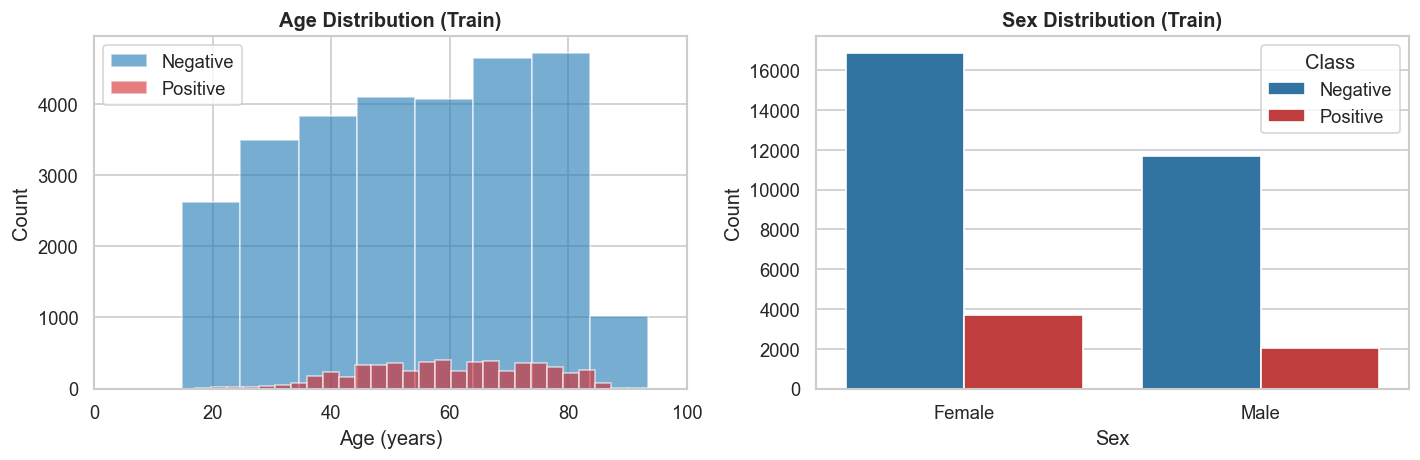
\includegraphics[width=0.95\linewidth]{img/dataset_demographics.png}
\caption[Age and sex distributions in the combined CODE-15\% +
SaMi-Trop training data before and after preprocessing]{Age and sex distributions in the combined CODE-15\% +
SaMi-Trop training data, after the preprocessing pipeline of
Section~\ref{sec:dataset}. Chagas-positive cases concentrate in
the 50--70-year band, reflecting the natural history of the
disease, while both sexes are represented across the adult age
range. Generated from the Approach~1 exploratory notebook.}
\label{fig:demographics}
\end{figure}

\subsection{Hardware and Computational Resources}
\label{sec:hardware}

All experiments were conducted on an Apple MacBook Pro with an M3 processor (11-core GPU, 18~GB unified memory), running PyTorch 2.10.0 with the Metal Performance Shaders (MPS) backend. This consumer-grade hardware choice was deliberate, aligning with the Green AI paradigm~\cite{lapicque2025greenai} discussed in Chapter~\ref{chap:sota}. The constraint imposed practical limitations: self-attention layers were disabled in diffusion model architectures due to MPS instability, and training times were capped at approximately 5 hours per experiment.

This hardware profile differs from the winning Challenge solutions: the first-place team employed Vision Transformer foundation models requiring multi-GPU clusters~\cite{santvliet2025detecting}, while the second-place team used Transformer-xLSTM ensembles with comparable resource demands~\cite{nicolson2025transformer}. The experimental program therefore asks whether domain knowledge and transfer learning can compensate for computational constraints.

\section{Evaluation Protocol and the Three Evaluation Groups}
\label{sec:eval_protocol}

The evaluation methodology was not constant across the sixteen approaches. Early iterations adopted a random split of the combined Brazilian data; later iterations recognized that this design contaminates the test set with the very out-of-distribution cohort (SaMi-Trop) on which generalization should be measured. As a result, the approaches fall into three evaluation groups that measure different quantities. These groups, together with the comparison rule that follows from them, must be borne in mind when reading any result in Section~\ref{sec:results_all}.

\subsection{Group A --- Mixed Random Split (Approaches 1--9)}

Approaches 1--9 used a random split of the mixed CODE-15\% and SaMi-Trop data. Approaches 1--2 used an 85\%/15\% train/validation split without a held-out test set, so their reported metrics were computed on the validation set used for model selection. Approaches 3--9 used a 70\%/15\%/15\% train/validation/test split, stratified by class label with a fixed random seed (42), yielding approximately 34,408 training, 7,372 validation, and 7,372 test samples (effective prevalence 16.7\%).

The defining characteristic of Group A is data contamination: because SaMi-Trop recordings were pooled with CODE-15\% before splitting, SaMi-Trop samples appear in the training, validation, and test partitions simultaneously (roughly 1,386 in training and 245 in the test set). The model therefore sees the out-of-distribution cohort during training, which inflates in-distribution test metrics and precludes any genuine assessment of cross-cohort generalization. This is the superseded methodology.

\subsection{Group B --- SaMi-Trop as Held-Out Test (Approach 10)}

Approach 10 was the first attempt at a clean out-of-distribution evaluation: the entire SaMi-Trop cohort (1,631 recordings) was held out as the test set, while training used CODE-15\% only. Because SaMi-Trop is 100\% Chagas positive, the test set contains a single class. Consequently, AUROC and the threshold-based Challenge Score are mathematically undefined for this group. Only validation metrics on CODE-15\% and, in principle, sensitivity on the single-class SaMi-Trop test set can be reported.

\subsection{Group C --- Patient-Grouped CODE-15\% Held-Out with Isolated OOD (Approaches 11, 12, 14, and 15)}

Approaches 11, 12, 14, and 15 adopted the cleanest protocol. CODE-15\% was split three ways using \texttt{GroupShuffleSplit} keyed on patient identifier (seed 42), guaranteeing that no patient appears in more than one partition. This yields an in-distribution held-out test set of approximately 7,129--7,134 samples (13.5--13.8\% Chagas prevalence). SaMi-Trop is fully isolated: it never participates in training, validation, or testing, and is used exclusively as an out-of-distribution (OOD) validation cohort. Because SaMi-Trop is single-class, only sensitivity (at one or more decision thresholds) is reported there, not AUROC.

\subsection{The Inviolable Comparison Rule}

\textbf{Metrics from Group A and Group C measure different things and must not be directly compared.} A Group A test score is an in-distribution estimate computed on a contaminated mixture; a Group C test score is a patient-disjoint in-distribution estimate, accompanied by a strictly isolated OOD sensitivity. Cross-tabulating the two would conflate an optimistically biased number with an unbiased one. The three groups are therefore tabulated separately, each table captioned with its test set, prevalence, sample count, and Challenge Score definition.

\subsection{Metrics and the Two Challenge Score Formulas}

Three complementary metrics are used: \textbf{AUROC} (threshold-independent discriminative ability), \textbf{AUPRC} (informative under class imbalance, focusing on the positive class~\cite{sameni2025geometry}), and \textbf{TPR@5\%} (true positive rate at 5\% false positive rate). The latter is the official PhysioNet Challenge 2025 metric, reflecting the clinically relevant screening operating point where false positives must be kept low.

A second, equally important caveat concerns the definition of the Challenge Score itself, which changed during the work:

\begin{itemize}
    \item \textbf{Approaches 1--3} predate the official metric and used a superseded composite, $0.5 \times \text{AUROC} + 0.5 \times \text{AUPRC}$. To avoid conflating the two, only AUROC and AUPRC are reported for these approaches.
    \item \textbf{Approaches 4 and later} use the official PhysioNet 2025 metric, TPR@5\% FPR, which directly measures screening capacity.
\end{itemize}

The two formulas are incompatible and are never tabulated together. Finally, bootstrap 95\% confidence intervals (1000 resamples, seed 42) were computed for the Group-C headline results (Approaches 11, 12, 14, 15) and for the test AUROC of Approach 7, providing an estimate of statistical uncertainty for the cleanest comparisons.

%%%%%%%%%%%%%%%%%%%%%%%%%%%%%%%%%%%%%%%%%%%%%%%%%%%%%%%%%%%%%%%%%%%%%%%%%%%%%

\section{Baseline Classifiers (Approaches 1--4)}
\label{sec:baseline}

The first four approaches establish a purely data-driven reference point against which every subsequent design is judged. They share a single 1-D ResNet backbone adapted for 12-lead ECG classification but differ in their training data, evaluation protocol, and loss formulation. The architecture is described first, followed by the iterative refinements through which cross-national confounding was removed, a proper held-out test set was introduced, and modern calibration techniques (focal loss, label smoothing, temperature scaling) were adopted.

\subsection{1-D ResNet Architecture}

The baseline classifier employed a one-dimensional Residual Network (ResNet)~\cite{he2016deep} adapted for 12-lead ECG classification. The architecture follows the design principles established by Ribeiro et al.~\cite{ribeiro2020automatic} for ECG analysis:

\begin{itemize}
    \item \textbf{Input:} 12-channel signal of 5,000 time steps ($12 \times 5000$).
    \item \textbf{Architecture:} 4 residual groups with 2 blocks each, base filter count of 64, kernel size 7, and dropout rate 0.3. Each residual block applies two 1D convolutions with batch normalization and ReLU activation, connected via a skip connection.
    \item \textbf{Output:} Global average pooling followed by a single sigmoid unit producing a Chagas probability $p \in [0, 1]$.
    \item \textbf{Parameters:} Approximately 8.8 million trainable parameters.
\end{itemize}
The residual connection mechanism $\mathbf{y} = \mathcal{F}(\mathbf{x}, \{W_i\}) + \mathbf{x}$ addresses vanishing gradients and enables effective training of deeper networks, which is essential for learning hierarchical temporal features across the 10-second ECG window.

\begin{figure}[htbp]
\centering
\begin{tikzpicture}[
    node distance=0.7cm,
    box/.style={
        draw, rounded corners, thick, align=left,
        text width=7.8cm, inner sep=6pt
    },
    smallbox/.style={
        draw, rounded corners, thick, align=center,
        text width=6.5cm, inner sep=4pt
    },
    arrow/.style={-{Latex[length=3mm]}, thick}
]
\node[smallbox] (input) {%
    \textbf{Input:} 12-lead ECG, $\mathbf{X} \in \mathbb{R}^{12 \times 5000}$
};
\node[box, below=of input] (stem) {%
    \textbf{Stem:} $\mathrm{Conv1D}(12 \to 64,\ \mathrm{kernel}=7) + \mathrm{BatchNorm} + \mathrm{ReLU}$
};
\node[box, below=of stem] (g1) {%
    \textbf{Residual Group 1} ($2$ blocks, $64$ filters) \\
    Block: $\mathrm{Conv} \to \mathrm{BN} \to \mathrm{ReLU}$;
    $\mathrm{Conv} \to \mathrm{BN}\,+\,\text{skip}$;
    $\mathrm{ReLU} \to \mathrm{Dropout}(0.3)$
};
\node[box, below=of g1] (g234) {%
    \textbf{Residual Groups 2, 3, 4} (same structure; progressive downsampling)
};
\node[smallbox, below=of g234] (gap) {Global Average Pooling};
\node[smallbox, below=of gap] (fc) {$\mathrm{Linear} \to \mathrm{sigmoid}$};
\node[smallbox, below=of fc] (output) {%
    Chagas probability $p \in [0,1]$
};
\draw[arrow] (input) -- (stem);
\draw[arrow] (stem) -- (g1);
\draw[arrow] (g1) -- (g234);
\draw[arrow] (g234) -- (gap);
\draw[arrow] (gap) -- (fc);
\draw[arrow] (fc) -- (output);
\end{tikzpicture}
\caption[One-dimensional ResNet baseline classifier (Approaches 1--4)]{One-dimensional ResNet baseline classifier (Approaches~1--4),
$\sim$8.8M parameters. Skip connection: $\mathbf{y} = \mathcal{F}(\mathbf{x}, \{W_i\}) + \mathbf{x}$.}
\label{fig:resnet_baseline}
\end{figure}

\subsection{Iterative Improvements}
\label{sec:baseline_evolution}

The baseline was refined through four iterative approaches, each addressing a specific limitation of its predecessor:

\textbf{Approach 1 (Baseline).} The initial model was trained on the full PhysioNet training set (including PTB-XL) with weighted binary cross-entropy loss ($\text{pos\_weight} = 10$) and an 85\%/15\% train/validation split. Evaluation used a single validation fold without a held-out test set, which precluded assessment of true generalization performance.

\textbf{Approach 2 (Pipeline Refinement).} Data loading bugs were corrected and age visualization artifacts were fixed. The refined pipeline confirmed reproducibility but underscored that incremental data fixes cannot overcome structural evaluation shortcomings.

\textbf{Approach 3 (Brazilian-Only Training with Test Set).} Two critical methodological changes were introduced: (1) PTB-XL was excluded from training, eliminating cross-national confounding in which the model could learn to distinguish German from Brazilian ECG characteristics rather than Chagas-specific features; (2) a proper train/validation/test split was established, providing the first unbiased generalization estimate within the contaminated Group-A protocol.

\textbf{Approach 4 (Training Optimization).} Three techniques were introduced to improve calibration and hard-example mining:

\begin{itemize}
    \item \textbf{Focal Loss}~\cite{lin2017focal} ($\alpha = 0.25$, $\gamma = 2.0$): Down-weights well-classified examples, focusing training on difficult cases near the decision boundary.
    \item \textbf{Label Smoothing}~\cite{muller2019does} ($\varepsilon = 0.1$): Prevents overconfident predictions by softening target labels from $\{0, 1\}$ to $\{\varepsilon/2, 1 - \varepsilon/2\}$.
    \item \textbf{Temperature Scaling}~\cite{guo2017calibration}: Post-hoc calibration of predicted probabilities using a learned temperature parameter on the validation set.
\end{itemize}

These changes improved calibration, lowering the optimal decision threshold from 0.95 (extreme overconfidence) to 0.34. Approach~4 is the first iteration to report the official TPR@5\% metric on the held-out test set, and it serves as the baseline against which all subsequent Group-A approaches are measured.

%%%%%%%%%%%%%%%%%%%%%%%%%%%%%%%%%%%%%%%%%%%%%%%%%%%%%%%%%%%%%%%%%%%%%%%%%%%%%

\section{Generative Data Augmentation (Approaches 5, 6, and 9)}
\label{sec:generative}

Because training optimization alone yielded only limited gains, generative models were investigated as a source of synthetic data augmentation. The hypothesis was that generating additional Chagas-positive ECG examples could improve minority-class recall without sacrificing specificity.

\subsection{Denoising Diffusion Probabilistic Models (Approach 5)}
\label{sec:ddpm}

A conditional Denoising Diffusion Probabilistic Model (DDPM)~\cite{ho2020denoising} was trained to generate synthetic 12-lead ECG signals conditioned on the Chagas disease label. The diffusion process defines a forward Markov chain that progressively corrupts data $\mathbf{x}_0$ into Gaussian noise over $T$ timesteps:

\begin{equation}
    q(\mathbf{x}_t | \mathbf{x}_{t-1}) = \mathcal{N}(\mathbf{x}_t; \sqrt{1 - \beta_t}\, \mathbf{x}_{t-1},\; \beta_t \mathbf{I})
\end{equation}

where $\{\beta_t\}_{t=1}^{T}$ is a cosine noise schedule~\cite{nichol2021improved}. A neural network $\epsilon_\theta(\mathbf{x}_t, t, y)$ is trained to predict the noise $\epsilon$ added at each step, enabling iterative denoising to generate new samples.

The noise prediction network was a conditional 1D U-Net~\cite{ronneberger2015unet} with the following specifications:

\begin{itemize}
    \item Base channels: 32, channel multipliers: $[1, 2]$, no self-attention (MPS constraint).
    \item Conditioning: sinusoidal timestep embedding + Adaptive Group Normalization (AdaGN) with class embedding.
    \item Classifier-Free Guidance~\cite{ho2022classifierfree}: 10\% class dropout during training; guidance scale $w = 2.0$ at inference.
    \item Sampling: DDIM~\cite{song2021denoising} with 25 steps and $\eta = 0$ for deterministic generation.
    \item Diffusion steps: $T = 500$, approximately 487,000 parameters.
\end{itemize}

After training, 500 synthetic Chagas-positive ECG recordings were generated via DDIM sampling. A quality filter retained only samples whose amplitude range and standard deviation fell within the 1st--99th percentile bounds of the training data. The retained synthetic positives were combined with the original training set to form an augmented dataset, on which a fresh ResNet classifier was retrained using the same configuration as Approach~4 (variant 5a). An alternative strategy used the diffusion model directly as a classifier by comparing reconstruction error under positive versus negative conditioning (variant 5b), with an ensemble of the two evaluated as variant 5c.

\subsection{Latent Diffusion Models (Approach 6)}
\label{sec:ldm}

Latent Diffusion Models (LDMs)~\cite{rombach2022highresolution} address the computational cost of pixel-space diffusion by operating in a compressed latent space. A 1D convolutional autoencoder was trained to compress the 12-lead ECG signal ($12 \times 5000$) into a lower-dimensional latent representation, achieving approximately 8$\times$ temporal compression. The encoder used strided convolutions and the decoder symmetric transposed convolutions, trained to minimize reconstruction loss on the ECG signals.

After autoencoder convergence, the latent diffusion model was trained with the same U-Net architecture and classifier-free guidance configuration as Approach~5, but operating on the compressed latent codes rather than raw signals. An additional physics-informed amplitude penalty constrained decoded samples to produce ECGs within physiologically plausible amplitude bounds derived from training-data percentiles. As with Approach~5, augmentation (variant 6a), direct latent-space classification (variant 6b), and their ensemble (variant 6c) were each evaluated.

\subsection{Adaptive Residual U-Net Architecture (Approach 9)}
\label{sec:adaptive_unet}

Approach~9 focused on architectural optimization of the diffusion model's noise prediction network, introducing \textbf{Adaptive Residual Blocks} (AdapResBlocks). In a standard residual block, the output is $\mathbf{y} = \mathbf{x} + \mathcal{F}(\mathbf{x})$. The adaptive variant introduces per-channel learnable scaling parameters $\boldsymbol{\alpha}$, initialized to zero:

\begin{equation}
    \mathbf{y} = \texttt{skip}(\mathbf{x}) + \boldsymbol{\alpha} \odot \mathcal{F}(\mathbf{x}), \quad \boldsymbol{\alpha} \in \mathbb{R}^{C},\; \boldsymbol{\alpha}_{\text{init}} = \mathbf{0}
\end{equation}

This initialization ensures that each block starts as a pure identity mapping, allowing the network to gradually learn which nonlinear transformations are beneficial. Combined with AdaGN conditioning and exponential-moving-average (EMA) weight averaging ($\text{decay} = 0.999$), the adaptive U-Net was trained for 50 epochs ($\sim$4 hours on M3). This approach did not include downstream classifier evaluation; its contribution is architectural. The generation quality of the resulting model is reported in Section~\ref{sec:results_groupA}. The AdapResBlock design was later adopted in the PINN architectures (Approaches 7, 8, and 10), where the zero-initialization property helped stabilize the joint optimization of classification and physics losses.

%%%%%%%%%%%%%%%%%%%%%%%%%%%%%%%%%%%%%%%%%%%%%%%%%%%%%%%%%%%%%%%%%%%%%%%%%%%%%

\section{Physics-Informed Approaches (Approaches 7, 8, and 10)}
\label{sec:pinn}

This section investigates whether incorporating electrophysiological domain knowledge through Physics-Informed Neural Networks (PINNs)~\cite{raissi2019physics} can improve classification performance, interpretability, or both. Three approaches were explored, progressing from a biophysical reaction-diffusion model to a phenomenological dynamical-systems model:

\begin{enumerate}
    \item \textbf{Approach 7:} Biophysical feature extraction using the Aliev-Panfilov model.
    \item \textbf{Approach 8:} Physics-Guided Diffusion Model (PGDM), combining Aliev-Panfilov physics with generative augmentation.
    \item \textbf{Approach 10:} Phenomenological feature extraction using the McSharry dynamical model.
\end{enumerate}

\subsection{Biophysical Model: Aliev-Panfilov PINN (Approach 7)}
\label{sec:aliev_panfilov}

Approach~7 grounds classification in a reaction-diffusion description of cardiac excitation, forcing all discriminative information through a three-parameter physical bottleneck. The following subsubsections introduce the Aliev-Panfilov equations and the electrophysiological meaning of their parameters, specify the encoder-decoder architecture that estimates them from a 12-lead ECG, define the composite classification-plus-physics training objective, and acknowledge the conceptual limitation of applying a spatial Laplacian across discrete leads.

\subsubsection{Theoretical Foundation}

The Aliev-Panfilov model~\cite{aliev1996simple} is a two-variable reaction-diffusion system describing cardiac action potential propagation:

\begin{align}
    \frac{\partial u}{\partial t} &= D \nabla^2 u + k\, u(1 - u)(u - a) - u \cdot v \label{eq:ap_u} \\
    \frac{\partial v}{\partial t} &= -\bigl(\epsilon_0 + \frac{\mu_1 v}{\mu_2 + u}\bigr)(v + k\, u(u - a - 1)) \label{eq:ap_v}
\end{align}

where $u$ represents the normalized membrane potential, $v$ the recovery variable, $D$ the diffusion coefficient (conduction velocity), $a$ the excitability threshold, and $k$ the repolarization rate. Three parameters carry direct electrophysiological meaning:

\begin{itemize}
    \item $D$: Quantifies conduction velocity, which is reduced in the fibrotic tissue characteristic of Chagas cardiomyopathy.
    \item $a$: Controls the excitability threshold, which is altered in regions with disrupted gap junctions.
    \item $k$: Governs repolarization kinetics, which are affected by ion channel remodeling.
\end{itemize}

\subsubsection{Architecture}

An encoder-decoder PINN was constructed with the following structure:

\begin{enumerate}
    \item \textbf{Encoder:} 1D convolutional stem ($12 \to 64$ channels, kernel size 15) followed by 4 Adaptive Residual Blocks, a strided downsampling convolution, and global average pooling.
    \item \textbf{Physics head:} A linear layer mapping the 64-dimensional global feature vector to 4 outputs, constrained via activation functions: $D$ (softplus, scale 20), $a$ (sigmoid, scale 0.25), $k_{\text{rep}}$ (softplus, scale 12), and $v_{\text{aux}}$ (tanh).
    \item \textbf{Classifier:} A two-layer MLP ($3 \to 32 \to 1$) operating \textit{exclusively} on the three physics parameters $(D, a, k)$, producing a single Chagas logit.
\end{enumerate}

The total parameter count was 522,473, approximately 17$\times$ smaller than the baseline ResNet (8.8M parameters).

The full architecture is summarised in
Figure~\ref{fig:aliev_panfilov_pinn}: a 1D convolutional encoder
with four Adaptive Residual Blocks and global average pooling
produces a 64-dimensional feature vector, which a linear physics
head projects onto the four electrophysiological outputs $(D, a,
k_{\text{rep}}, v_{\text{aux}})$ via biophysically motivated
activation functions; the classifier MLP $(3{\to}32{\to}1)$ then
operates exclusively on the three interpretable parameters $(D, a,
k)$, so all discriminative information must pass through the
physics bottleneck. The composite loss enforces the
Aliev--Panfilov PDE residual on the lead-averaged signal, as
defined in Section~\ref{sec:aliev_panfilov}.

\begin{figure}[htbp]
\centering
\begin{tikzpicture}[
    node distance=0.9cm,
    box/.style={
        draw, rounded corners, thick, align=left,
        text width=8.2cm, inner sep=7pt
    },
    smallbox/.style={
        draw, rounded corners, thick, align=center,
        text width=6.5cm, inner sep=4pt
    },
    arrow/.style={-{Latex[length=3mm]}, thick}
]
\node[smallbox] (input) {%
    \textbf{Input:} 12-lead ECG, $\mathbf{X} \in \mathbb{R}^{12 \times 5000}$
};
\node[box, below=of input] (encoder) {%
    \textbf{Encoder} \\[2pt]
    $\mathrm{Conv1D}(12 \to 64,\ \mathrm{kernel}=15) + \mathrm{BatchNorm} + \mathrm{ReLU}$ \\
    $4 \times$ Adaptive Residual Blocks $(64\ \text{ch})$ \\
    Strided downsampling convolution \\
    Global Average Pooling
};
\node[smallbox, below=of encoder] (features) {%
    64-dimensional feature vector, $\mathbf{z} \in \mathbb{R}^{64}$
};
\node[box, below=of features] (physics) {%
    \textbf{Physics head:} $\mathrm{Linear}(64 \to 4)$ \\[2pt]
    $D$ \hfill softplus, scale $20$ \\
    $a$ \hfill sigmoid, scale $0.25$ \\
    $k_{\text{rep}}$ \hfill softplus, scale $12$ \\
    $v_{\text{aux}}$ \hfill $\tanh(\cdot)$
};
\node[smallbox, below=of physics] (params) {%
    Three physics parameters, $\boldsymbol{\theta} = (D,\ a,\ k_{\text{rep}})$
};
\node[smallbox, below=of params] (classifier) {%
    Classifier MLP: $3 \to 32 \to 1$
};
\node[smallbox, below=of classifier] (output) {%
    \textbf{Chagas logit} $\hat{y} \in \mathbb{R}$
};
\draw[arrow] (input) -- (encoder);
\draw[arrow] (encoder) -- (features);
\draw[arrow] (features) -- (physics);
\draw[arrow] (physics) -- (params);
\draw[arrow] (params) -- (classifier);
\draw[arrow] (classifier) -- (output);
\end{tikzpicture}
\caption[Aliev--Panfilov Physics-Informed Neural Network]{Aliev--Panfilov Physics-Informed Neural Network
(Approach~7). The classifier operates only on the three
interpretable parameters $(D, a, k)$.}
\label{fig:aliev_panfilov_pinn}
\end{figure}

\subsubsection{Training Objective}

The model was trained with a composite loss:

\begin{equation}
    \mathcal{L} = \mathcal{L}_{\text{cls}} + \lambda_{\text{EP}} \cdot \mathcal{L}_{\text{EP}}
\end{equation}

where $\mathcal{L}_{\text{cls}}$ is the focal loss for Chagas disease classification, and $\mathcal{L}_{\text{EP}}$ is the physics residual:

\begin{equation}
    \mathcal{L}_{\text{EP}} = \frac{1}{T'} \sum_{t=2}^{T'-1} \left( \frac{du}{dt}\bigg|_t - D \cdot \nabla^2_{\text{leads}} u_t - k \cdot u_t(1-u_t)(u_t - a) + u_t \cdot v \right)^2
\end{equation}

Here $u(t)$ is the lead-averaged ECG waveform (min-max normalized to $[0,1]$), $du/dt$ is computed via central finite differences, and $\nabla^2_{\text{leads}}$ approximates the spatial Laplacian using circular second differences across the 12 leads. The physics weight was set to $\lambda_{\text{EP}} = 0.05$.

\subsubsection{Methodological Caveat}

A conceptual limitation must be acknowledged: applying the spatial diffusion operator $\nabla^2$ across discrete ECG leads treats the 12 leads as a spatial domain, which lacks rigorous physical justification. The 12-lead ECG represents projections of a single cardiac dipole vector onto different axes, not spatially distributed measurements of membrane potential. Despite this approximation, the physics loss served as an effective regularizer, constraining the encoder to extract features consistent with Aliev-Panfilov dynamics. This caveat recurs in the PGDM (Approach 8), which evaluates the same residual on representative leads.

\subsection{Physics-Guided Diffusion Model (Approach 8)}
\label{sec:pgdm}

Approach 8 combined the Aliev-Panfilov physics constraint with diffusion-based generative augmentation, creating a Physics-Guided Diffusion Model (PGDM). The PGDM extends the conditional DDPM (Approach 5) by adding an electrophysiology loss term to the diffusion training objective:

\begin{equation}
    \mathcal{L}_{\text{PGDM}} = \underbrace{\| \epsilon - \epsilon_\theta(\mathbf{x}_t, t, y) \|^2}_{\text{noise prediction}} + \lambda_{\text{EP}} \cdot \underbrace{\mathbb{E}\bigl[r_u^2 + r_v^2\bigr]}_{\text{Aliev-Panfilov residual}}
\end{equation}

The physics residual is computed on the Tweedie estimate of the clean signal $\hat{\mathbf{x}}_0$ derived from the current noise prediction. The Aliev-Panfilov residuals $r_u$ and $r_v$ are evaluated on leads II and V1 (selected as representative of inferior and precordial lead groups), using the same finite-difference scheme as Approach~7 with $\lambda_{\text{EP}} = 0.05$. The same caveat regarding the spatial operator on leads (Section~\ref{sec:aliev_panfilov}) applies. The trained PGDM was used identically to Approach~5: generating synthetic Chagas-positive ECGs, filtering for quality, and retraining a ResNet classifier on the augmented dataset.

\subsection{Phenomenological Model: McSharry PINN (Approach 10)}
\label{sec:mcsharry}

Approach~10 replaces the spatial reaction-diffusion description used in Approach~7 with a phenomenological limit-cycle oscillator that is mathematically appropriate for a single-channel ECG. The subsubsections that follow motivate this change, present the 17-parameter McSharry generative model with its five Gaussian P/Q/R/S/T attractors, describe the corresponding PINN architecture and ODE-residual training loss, and explain the shift to a Group~B evaluation protocol in which SaMi-Trop is held out as a single-class out-of-distribution test set.

\subsubsection{Motivation}

The Aliev-Panfilov model's conceptual limitation, namely applying a spatial PDE to non-spatial ECG leads, motivated a different modeling approach. The McSharry dynamical model~\cite{mcsharry2003dynamical} treats the ECG not as a spatial field but as the output of a limit-cycle oscillator in phase space $(\phi, z)$, where the angular variable $\phi$ traverses the cardiac cycle and $z(t)$ represents the ECG voltage.

\subsubsection{Model Formulation}

The McSharry model generates an ECG-like waveform by summing Gaussian contributions from five characteristic waves (P, Q, R, S, T):

\begin{equation}
    \frac{dz}{dt} = -\sum_{i \in \{P,Q,R,S,T\}} a_i \cdot \Delta\theta_i \cdot \exp\!\left(-\frac{\Delta\theta_i^2}{2b_i^2}\right) - (z - z_0)
    \label{eq:mcsharry}
\end{equation}

where $\Delta\theta_i = \text{atan2}(\sin(\theta - \theta_i), \cos(\theta - \theta_i))$ is the wrapped angular distance from the $i$-th wave center, $a_i$ is the amplitude, $b_i$ the width, and $\theta_i$ the phase of each Gaussian attractor. Together with the heart rate $f$ and baseline offset $z_0$, this yields 17 interpretable parameters: $\{f, z_0, a_P, b_P, \theta_P, \dots, a_T, b_T, \theta_T\}$.

\subsubsection{Architecture and Training}

The PINN architecture mirrors Approach~7, with the physics head modified to produce 17 McSharry parameters instead of 3 Aliev-Panfilov parameters. Heart rate $f$ is constrained by a sigmoid scaled to $[0.5, 2.5]$~Hz (30--150~bpm); $z_0$ and the amplitudes $a_i$ are tanh-scaled; the widths $b_i$ are softplus-scaled (strictly positive); and the phases $\theta_i$ are constrained to $[-\pi, \pi]$ via $\pi \cdot \tanh(\cdot)$. The classifier MLP operates on the full 17-parameter vector ($17 \to 32 \to 1$), for a total of 522,422 parameters. The composite loss combines focal classification loss with the McSharry ODE residual:

\begin{equation}
    \mathcal{L} = \mathcal{L}_{\text{cls}} + \lambda_{\text{ODE}} \cdot \mathcal{L}_{\text{ODE}}
\end{equation}

where $\mathcal{L}_{\text{ODE}}$ is the mean squared residual of Equation~\ref{eq:mcsharry} evaluated on the lead-averaged ECG waveform via central finite differences. The ODE weight $\lambda_{\text{ODE}} = 0.1$ was set higher than in the Aliev-Panfilov experiment, reflecting the stronger theoretical grounding of the McSharry model for 1D ECG signals.

For reproducibility, Table~\ref{tab:pinn_hyperparams} centralizes the neural-network hyperparameters used to train the four PINN-family models (Approaches~7, 8, 10, 11). Optimizer, learning rate, weight decay, batch size, epoch count, and physics-loss coefficient are reported for each.

\begin{table}[htbp]
\centering
\small
\caption[Neural-network hyperparameters for the four PINN-family approaches]{Neural-network hyperparameters for the four PINN-family approaches. All approaches use AdamW with gradient clipping at $1.0$ and focal classification loss ($\alpha = 0.25$, $\gamma = 2.0$, except where noted). The ``Physics loss'' row gives the term added to the classification loss and its coefficient.}
\label{tab:pinn_hyperparams}
\begin{tabular}{@{}p{3.0cm} p{2.4cm} p{2.6cm} p{2.4cm} p{2.4cm}@{}}
\hline
Approach & \textbf{7} & \textbf{8} & \textbf{10} & \textbf{11} \\
\hline
\multicolumn{5}{@{}l@{}}{\textit{Training}} \\
Optimizer            & AdamW   & AdamW    & AdamW   & AdamW \\
Learning rate        & $10^{-3}$ & $2{\times}10^{-4}$ & $10^{-3}$ & $10^{-3}$ \\
Weight decay         & $10^{-4}$ & $10^{-6}$ & $10^{-4}$ & $10^{-4}$ \\
Batch size           & 16      & 8$^{\dagger}$ & 16  & 16 \\
Epochs               & 40      & 50       & 40      & 40 \\
LR schedule          & Lin.\,warmup + cos. & Lin.\,warmup + cos. & Lin.\,warmup + cos. & Cosine \\
Warmup epochs        & 2       & 3        & 2       & --- \\
Grad.\ clip          & 1.0     & 1.0      & 1.0     & 1.0 \\
\hline
\multicolumn{5}{@{}l@{}}{\textit{Architecture}} \\
Encoder stem         & $12{\to}64$, k15 & U-Net 32\,ch$^{\ddagger}$ & $12{\to}64$, k15 & $12{\to}64$, k15 \\
Depth                & 4 AdapRes & 2 levels & 4 AdapRes & 4 AdapRes \\
Total parameters     & 522{,}473 & --- & 522{,}422 & --- \\
\hline
\multicolumn{5}{@{}l@{}}{\textit{Physics term}} \\
Term added           & AP residual & AP residual & McSharry ODE & Reconstruction\newline MSE \\
Coefficient          & $\lambda_{\text{EP}}{=}0.05$ & $\lambda_{\text{EP}}{=}0.05$ & $\lambda_{\text{ODE}}{=}0.1$ & $\lambda{=}1.0$ \\
\hline
\multicolumn{5}{@{}l@{}}{\footnotesize $^{\dagger}$ Effective batch size 16 with gradient accumulation $\times 2$.} \\
\multicolumn{5}{@{}l@{}}{\footnotesize $^{\ddagger}$ Approach~8 retrains a separate ResNet classifier on the PGDM-augmented data.} \\
\end{tabular}
\end{table}

\subsubsection{Evaluation Design}

Approach~10 was the first to break with the Group-A protocol: it trained on CODE-15\% only and held out the entire SaMi-Trop cohort as the test set (Group B, Section~\ref{sec:eval_protocol}). The single-class test set renders AUROC undefined, so only validation metrics on CODE-15\% and OOD sensitivity can be reported. The contrast between this approach and the foundation-model approaches is taken up in the discussion in Chapter~\ref{chap:conclusions}.

%%%%%%%%%%%%%%%%%%%%%%%%%%%%%%%%%%%%%%%%%%%%%%%%%%%%%%%%%%%%%%%%%%%%%%%%%%%%%

\section{Phenomenological Structured Autoencoder (Approach 11)}
\label{sec:autoencoder}

Approach~11 is a sibling iteration of Approach~10: both use the McSharry phenomenological model to parametrize the ECG, but Approach~11 organizes the network as a structured autoencoder with a two-term objective (classification plus reconstruction). It is the first approach to adopt the Group-C protocol (patient-grouped CODE-15\% held-out with strictly isolated SaMi-Trop OOD).

\subsection{Architecture}

The encoder reuses the EAND-ARN design: a convolutional stem ($12 \to 64$, kernel size 15) with GroupNorm and GELU, followed by four AdapResBlocks (residual blocks with a learned $\alpha$, GroupNorm, GELU, dropout 0.2), a strided downsampling convolution, and temporal mean pooling, producing a 64-dimensional context vector. An ODE head maps this context to 82 physical parameters describing a single ``median'' cardiac beat: 5 global Gaussian widths $b$, 5 global phases $\theta$ (chained chronologically P$\to$Q$\to$R$\to$S$\to$T, with the R phase fixed at $t=0$ and the remaining phases forced into chronological order by softplus-scaled differences), 60 amplitudes $a$ (12 leads $\times$ 5 waves), and 12 per-lead baselines $z_0$.

The classifier is gray-box by design: a two-layer MLP ($83 \to 32 \to 1$) that operates on the 82 McSharry parameters concatenated with a deterministically computed heart rate $\text{hr}_f$ (83 inputs total). It receives no direct signal from the encoder context vector, so all discriminative information must pass through the interpretable physical parametrization.

\subsection{Training Objective}

The total loss combines a focal classification term ($\alpha = 0.25$, $\gamma = 2.0$) with a reconstruction term:

\begin{equation}
    \mathcal{L} = \mathcal{L}_{\text{cls}} + \lambda \cdot \mathcal{L}_{\text{recon}}, \qquad \lambda = 1.0
\end{equation}

The reconstruction loss is the mean squared error between an analytic 12-lead signal (the sum of five Gaussian functions in phase space, with $\theta(t) = 2\pi f t$) and the empirical \texttt{median\_beat}, enforcing physical interpretability of the parameters. Training used AdamW (lr $10^{-3}$, weight decay $10^{-4}$), CosineAnnealingLR, gradient clipping at 1.0, batch size 16, and 40 epochs, with the best checkpoint selected on validation AUROC.

\subsection{Design Limitations}

Three design limitations follow. First, the gray-box constraint sacrifices discriminative power, because the classifier discards the encoder context and cannot exploit micro-morphological variation that a sum of five Gaussians fails to represent (for example, QRS fragmentation). Second, the widths $b$ and phases $\theta$ are shared across all 12 leads, which is anatomically inexact given the heart's electrical axis but stabilizes training. Third, operating on a median beat discards heart-rate variability, retaining only $\text{hr}_f$; this is defensible for Chagas, whose ECG signature is primarily morphological (RBBB, LAFB).

%%%%%%%%%%%%%%%%%%%%%%%%%%%%%%%%%%%%%%%%%%%%%%%%%%%%%%%%%%%%%%%%%%%%%%%%%%%%%

\section{Self-Supervised and Foundation-Model Approaches (Approaches 12, 14, and 15)}
\label{sec:foundation}

The final family of approaches abandons training from scratch in favor of transfer learning from large pretrained ECG models. As discussed in Chapter~\ref{chap:sota}, self-supervised pretraining and ECG foundation models~\cite{mckeen2024ecgfm,li2024ecgfounder,song2024foundation} have emerged as a dominant paradigm. All three approaches in this section follow the Group-C protocol.

\subsection{DeepECG-SSL Fine-Tuning (Approach 12)}
\label{sec:deepecg_ssl}

Approach~12 uses a pretrained self-supervised model, DeepECG-SSL, as a feature extractor. DeepECG-SSL adopts a wav2vec~2.0 architecture~\cite{vaswani2017attention} (a convolutional feature extractor of four stride-2 layers followed by a 12-layer Transformer producing 768-dimensional embeddings) pretrained contrastively on roughly 1.9 million ECGs from the CODE-15 database. The encoder output sequence is reduced by global mean pooling to a single 768-dimensional vector, on top of which a classification head is added: $\text{Linear}(768 \to 128) \to \text{GELU} \to \text{Dropout}(0.2) \to \text{Linear}(128 \to 1)$.

Training proceeds in two stages. Stage~A performs \textbf{linear probing}: the encoder is frozen and only the head is trained (10 epochs, lr $10^{-3}$). Stage~B performs full \textbf{fine-tuning}: the entire model is unfrozen and trained at a much smaller learning rate (lr $10^{-5}$) with early stopping (patience 5). The loss is focal loss with $\alpha \approx 0.86$ (set dynamically from class frequencies) and $\gamma = 2.0$. The contrast between the frozen linear probe and the fine-tuned model isolates how much task-specific adaptation contributes beyond the pretrained representations. As DeepECG-SSL was pretrained on the same CODE-15 corpus as the downstream training data, this approach probes the upper bound of in-distribution transfer.

\subsection{Hybrid Foundation Model + McSharry PINN (Approach 14)}
\label{sec:hybrid}

Approach~14 combines two sources of ECG knowledge: the deep latent representation of the ECGFounder foundation model~\cite{li2024ecgfounder} and the morphological parameters extracted by the McSharry PINN trained in Approach~10. Both branches are used as frozen feature extractors; only a projection layer and a final MLP classifier are trained.

\begin{itemize}
    \item \textbf{ECGFounder branch:} A Net1D model pretrained on more than 10 million ECGs across 150 clinical labels (RBBB, LAFB, LVH, AF, and others), producing a 1024-dimensional embedding, projected through $\text{Linear}(1024 \to 128)$ with LayerNorm and GELU.
    \item \textbf{PINN branch:} The frozen encoder from Approach~10 (\texttt{approach10\_mcsharry\_best.pt}) producing 17 McSharry parameters as a compressed morphological representation, projected through $\text{Linear}(17 \to 128)$ with LayerNorm and GELU.
    \item \textbf{Fusion:} The two 128-dimensional projections are concatenated to 256 dimensions, then passed through $\text{Linear}(256 \to 64)$ (LayerNorm, GELU, dropout 0.3) and $\text{Linear}(64 \to 1)$. Equal projection widths prevent the high-dimensional ECGFounder branch from dominating the 17-dimensional PINN branch.
\end{itemize}

Training used AdamW (lr $10^{-4}$), a 3-epoch warmup with cosine annealing, focal loss ($\alpha = 0.862$, $\gamma = 2.0$), and 20 epochs.

The full architecture is summarised in
Figure~\ref{fig:hybrid_foundation_pinn}: the 12-lead input feeds
two frozen feature extractors in parallel; both feature streams
are projected to equal-width 128-dimensional vectors (to prevent
the high-dimensional ECGFounder branch from dominating the
17-dimensional PINN branch), concatenated into a 256-dimensional
fused representation, and passed through a small MLP that produces
the final Chagas logit. Only the projection layers and the fusion
MLP are trained; both feature extractors remain frozen. The PINN
branch contributes a low-dimensional morphological summary, while
the ECGFounder branch contributes a high-dimensional
clinical-label embedding.

\begin{figure}[htbp]
\centering
\begin{tikzpicture}[
    node distance=0.7cm and 0.25cm,
    box/.style={
        draw, rounded corners, thick, align=center,
        text width=4.2cm, inner sep=4pt, font=\small
    },
    smallbox/.style={
        draw, rounded corners, thick, align=center,
        text width=4.2cm, inner sep=3pt, font=\small
    },
    widebox/.style={
        draw, rounded corners, thick, align=center,
        text width=6.4cm, inner sep=4pt, font=\small
    },
    arrow/.style={-{Latex[length=2.5mm]}, thick}
]
\node[widebox] (input) {%
    \textbf{Input:} 12-lead ECG, $\mathbf{X} \in \mathbb{R}^{12 \times 5000}$
};
\node[box, below left=0.9cm and 0.05cm of input] (ecgfounder) {%
    \textbf{ECGFounder} (Net1D, frozen) \\
    $10\mathrm{M}{+}$ ECG, $150$ labels \\
    $\to 1024$-dim.\ embedding
};
\node[box, below right=0.9cm and 0.05cm of input] (mcsharry) {%
    \textbf{McSharry PINN} (Approach~10, frozen) \\
    Encoder $\to 4{\times}$ AdapRes \\
    $\to$ physics head
};
\node[smallbox, below=of ecgfounder] (ecgproj) {%
    $\mathrm{Linear}(1024 \to 128)$ \\ $+\,\mathrm{LN} + \mathrm{GELU}$
};
\node[smallbox, below=of mcsharry] (params) {%
    17 McSharry parameters \\ $\boldsymbol{\theta}_{\mathrm{M}} \in \mathbb{R}^{17}$
};
\node[smallbox, below=of params] (physproj) {%
    $\mathrm{Linear}(17 \to 128)$ \\ $+\,\mathrm{LN} + \mathrm{GELU}$
};
\node[widebox, below=0.9cm of $(ecgproj)!0.5!(physproj)$] (concat) {%
    Concatenate $\to 256$-dim.\ vector \\ $\mathbf{h} = [\mathbf{h}_{\mathrm{ECG}};\,\mathbf{h}_{\mathrm{PINN}}] \in \mathbb{R}^{256}$
};
\node[widebox, below=of concat] (fusion) {%
    $\mathrm{Linear}(256 \to 64) + \mathrm{LN} + \mathrm{GELU} + \mathrm{Dropout}(0.3)$
};
\node[widebox, below=of fusion] (classifier) {%
    $\mathrm{Linear}(64 \to 1)$
};
\node[widebox, below=of classifier] (output) {%
    \textbf{Chagas logit} $\hat{y} \in \mathbb{R}$
};
\coordinate (split) at ($(input.south) + (0,-0.3)$);
\draw[arrow] (input.south) -- (split);
\draw[arrow] (split) -| (ecgfounder.north);
\draw[arrow] (split) -| (mcsharry.north);
\draw[arrow] (ecgfounder) -- (ecgproj);
\draw[arrow] (mcsharry) -- (params);
\draw[arrow] (params) -- (physproj);
\draw[arrow] (ecgproj.south) |- (concat.west);
\draw[arrow] (physproj.south) |- (concat.east);
\draw[arrow] (concat) -- (fusion);
\draw[arrow] (fusion) -- (classifier);
\draw[arrow] (classifier) -- (output);
\end{tikzpicture}
\caption[Approach 14 hybrid architecture (frozen ECGFounder + McSharry PINN)]{Approach~14 hybrid architecture. Two frozen feature
extractors are projected to equal-width 128-dimensional vectors
and concatenated; only the fusion MLP is trained.}
\label{fig:hybrid_foundation_pinn}
\end{figure}

Two methodological caveats must accompany any description of this model. First, the McSharry PINN here is a \emph{frozen black-box encoder}, not an active physics module: all physics-supervised training (the McSharry ODE residual) occurred in Approach~10. The correct framing is that morphological features extracted by a physics-supervised PINN are reused; the hybrid model itself should not be described as ``physics-informed''. Second, because the McSharry ODE is defined for a single lead while the PINN ingests all 12 leads, its 17 outputs are a compressed multi-lead representation that carries morphological semantics only incidentally and does not correspond to physiologically interpretable single-beat parameters.

\subsection{DeepECG-SSL with Temporal Attention (Approach 15)}
\label{sec:attention}

Approach~15 extends Approach~12 by replacing global mean pooling with a learned temporal-attention mechanism~\cite{vaswani2017attention}. The frozen DeepECG-SSL encoder produces a sequence of 768-dimensional vectors, one per time step. Rather than averaging them, a single learned query vector $(1, 1, 768)$ attends over the sequence (cross-attention with the sequence as keys and values), yielding both a pooled 768-dimensional representation and an attention-weight vector $(B, 1, T)$ that constitutes a temporal saliency map. The classification head is identical to the Approach~12 linear probe: $\text{LayerNorm}(768) \to \text{Linear}(768 \to 128) \to \text{GELU} \to \text{Dropout}(0.2) \to \text{Linear}(128 \to 1)$.

Because the encoder remains frozen and only the query and head are trained, the model is heavily regularized and trains stably across all 20 epochs without the rapid overfitting observed under full fine-tuning. Training used AdamW (lr $10^{-4}$, weight decay $10^{-4}$), focal loss ($\alpha = 0.25$, $\gamma = 2.0$), and batch size 32. The attention weights afford a form of interpretability distinct from the parameter-importance analysis of Approaches 10 and 11: they indicate \emph{when} in the cardiac cycle the model attends, rather than \emph{which} morphological feature it relies upon, enabling saliency heatmaps over the ECG waveform.

%%%%%%%%%%%%%%%%%%%%%%%%%%%%%%%%%%%%%%%%%%%%%%%%%%%%%%%%%%%%%%%%%%%%%%%%%%%%%

\section{Incomplete Experiments (Approaches 13 and 16)}
\label{sec:incomplete}

Two further experiments were designed but not completed. They are described here for the sake of a faithful account of the research program; no performance metrics are available for either, and none should be inferred.

\subsection{ECGFounder with Interpretable Clinical Features (Approach 13)}

Approach~13 was intended to combine the ECGFounder foundation model~\cite{li2024ecgfounder} with a gradient-boosted tree classifier (XGBoost) operating on interpretable clinical features, in the spirit of concept-bottleneck models~\cite{koh2020concept}. The design called for ECGFounder to predict its 150 clinical labels (such as RBBB, LAFB, and LVH) as intermediate concepts, from which a small set of interpretable features would be derived and fed to XGBoost for Chagas classification, with SHAP attribution providing post-hoc explanation.

This design was not realized. Inspection of the notebook file\\ \texttt{approach13\_ecgfounder\_interpretable.ipynb} shows that only cells 1--3 executed (library imports and loading of the ECGFounder model); the subsequent cells responsible for data loading, feature extraction, XGBoost/logistic-regression training, evaluation, and SHAP analysis were never run (their execution counts are null). No model files (\texttt{.pkl}) or feature caches (\texttt{.npz}) were produced, and the SHAP cell still contained a placeholder \texttt{TODO} for the ECGFounder label names. The approach therefore remains conceptually interesting but unrealized; it is recorded here as future work. The full notebook source is reproduced in Appendix~\ref{app:approach13} and is also available in the accompanying repository at \url{https://github.com/puszekjuliuszek/magisterka}.

\subsection{Cross-Domain PTB-XL Generalization Probe (Approach 16)}

Approach~16 was not a new classifier but a \emph{diagnostic, falsificationist experiment}. Its goal was to test whether the best fine-tuned foundation model (Approach~12) had learned a genuine Chagas disease signature or merely the shortcut ``RBBB/LAFB $\approx$ Chagas''. Because chronic Chagas cardiomyopathy diffusely damages the conduction system, right bundle branch block (RBBB) and left anterior fascicular block (LAFB) are among its earliest electrocardiographic manifestations and correlate strongly with Chagas in the Brazilian training cohort. However, these conduction abnormalities are also common in the general population for unrelated reasons (coronary disease, valvular disease, pulmonary disease, athletic variants). A model that learned the shortcut would exhibit an elevated false-positive rate in a non-endemic population, concentrated in RBBB/LAFB subgroups.

The intended design used PTB-XL, a German cohort with effectively 0\% Chagas disease prevalence, where every positive prediction is, by definition, a false positive. The Approach~12 model would be applied to PTB-XL recordings, with the decision threshold fixed by Youden's J on the Brazilian validation set, and the false-positive rate compared across four subgroups (RBBB+, LAFB+, both, and neither), parsed from the SCP-ECG annotations. A uniform low false-positive rate would indicate a genuine signature; a higher rate in the RBBB/LAFB subgroups would indicate shortcut learning.

This experiment did not complete. The classifier-head weights file\\ (\texttt{approach12\_finetune\_code15\_best.pt}) was absent from the notebook's working directory at runtime, so the inference and threshold-selection cells were never executed; only the PTB-XL data-loading cell ran, confirming that 2,783 PTB-XL recordings were present in the cache. Running the notebook without the head weights would have left the classifier randomly initialized, making any resulting false-positive rates artifacts rather than a test of Approach~12. The cross-domain generalization probe is therefore reported as a sound but unexecuted design, consistent with the hidden-stratification concerns raised in the medical machine-learning literature.

%%%%%%%%%%%%%%%%%%%%%%%%%%%%%%%%%%%%%%%%%%%%%%%%%%%%%%%%%%%%%%%%%%%%%%%%%%%%%

The remainder of this chapter reports the quantitative findings for the sixteen approaches, organized by the three evaluation groups introduced in Section~\ref{sec:eval_protocol}.

%%%%%%%%%%%%%%%%%%%%%%%%%%%%%%%%%%%%%%%%%%%%%%%%%%%%%%%%%%%%%%%%%%%%%%%%%%%%%

\section{Results}\label{sec:results_all}
\label{chap:results}

The results are organized by the three evaluation groups defined
in Section~\ref{sec:eval_protocol}. Each group used a different
test set, prevalence, and Challenge Score formulation, so the groups
are reported in three separate tables. Cross-group comparison is invalid: a
metric from Group~A cannot be placed alongside a metric from Group~C, because
the underlying test populations, contamination status, and scoring conventions
differ. Within each table the values are directly comparable; across tables they
are not.

\subsection{Group A: Random-Split Evaluation (Approaches 1--9)}\label{sec:results_groupA}

Group~A comprises the baseline classifiers, the generative-augmentation
variants, and the early physics-informed models. All were evaluated on the
mixed random-split test set of approximately $7{,}372$ samples at $16.7\%$
Chagas prevalence. This split was contaminated by SaMi-Trop recordings and
reflects the earlier experimental methodology. For Approaches~1--3 only AUROC
and AUPRC are reported because these experiments predate the adoption of the
PhysioNet~2025 Challenge Score (true-positive rate at $5\%$ false-positive rate,
TPR@5\%); the TPR@5\% column therefore shows ``---'' for those
rows.\footnote{Approaches~1 and~2 were also evaluated on a single
validation fold without a held-out test set; Approach~3 first introduced a
proper train/validation/test split (Section~\ref{sec:baseline_evolution}).
Together with the superseded composite score, this means the first three
rows of Table~\ref{tab:groupA} differ from later Group~A rows in both
\emph{metric} and \emph{evaluation design}, and should be read as
preliminary baselines rather than as directly comparable Group~A results.}
Approaches~4 and later report TPR@5\% as the Challenge Score; Approach~9 is a
generation-only model and reports no classifier metrics. The complete
Group~A results, computed on the mixed random-split test set ($\approx 7{,}372$
samples, $16.7\%$ Chagas prevalence, SaMi-Trop contaminated), are presented in
Table~\ref{tab:groupA}.

\begin{table}[htbp]
\centering
\caption{Group~A results for Approaches 1--9.}
\label{tab:groupA}
\begin{tabular}{c l c c c}
\hline
\textbf{Approach No.} & \textbf{Approach name} & \textbf{AUROC} & \textbf{AUPRC} & \textbf{TPR@5\%} \\
\hline
1   & ResNet baseline (val)            & 0.8138 & 0.5063 & --- \\
2   & ResNet + calibration (val)       & 0.8162 & 0.5202 & --- \\
3   & Brazilian-only ResNet            & 0.8008 & 0.4895 & --- \\
4   & Focal + label smoothing + temp.  & 0.8087 & 0.5099 & 0.2164 \\
5a  & ResNet + DDPM augmentation       & 0.8116 & 0.5244 & 0.2197 \\
5b  & DDPM as classifier               & 0.6080 & 0.2661 & 0.1221 \\
5c  & Ensemble (5a + 5b)               & 0.8116 & 0.5244 & 0.2197 \\
6a  & ResNet + LDM augmentation        & 0.8133 & 0.5146 & 0.2172 \\
6b  & LDM as classifier                & 0.7609 & 0.4262 & 0.1888 \\
6c  & Ensemble (6a + 6b)               & 0.7841 & 0.4957 & 0.2181 \\
7   & Aliev--Panfilov PINN             & 0.8165 & 0.5361 & 0.2210 \\
8   & PGDM                             & 0.8148 & 0.5415 & 0.2289 \\
9   & Adaptive U-Net (generation only) & N/A    & N/A    & N/A    \\
\hline
\end{tabular}
\end{table}

The baseline progression from Approach~1 through Approach~4 shows the AUROC
plateauing near $0.81$, with the AUPRC remaining around $0.51$. The Approach~7
test AUROC of $0.8165$ carries a bootstrap $95\%$ confidence interval of
$[0.8028, 0.8295]$ (notebook cell~16). Generative data augmentation produced
only marginal gains: Approach~5a (DDPM augmentation, $0.8116/0.5244/0.2197$) and
Approach~6a (LDM augmentation, $0.8133/0.5146/0.2172$) improved negligibly over
the Approach~4 baseline ($0.8087/0.5099/0.2164$). The two generative models
used directly as classifiers performed worse than the augmented discriminative
baselines; in particular, Approach~5b ($0.6080/0.2661/0.1221$) is a genuine but
weaker discriminative classifier, not a degenerate all-positive predictor. The
physics-informed Approaches~7 and~8 yielded the strongest Group~A Challenge
Scores, with Approach~8 (PGDM) attaining the highest Challenge Score in the
group at $0.2289$. No independent PGDM-specific test cell with stored
predictions exists for Approach~8, so a bootstrap confidence interval is not
computable for that row. Approach~9 is a generative model only: it produced no
classifier metrics, reaching a train-on-synthetic / test-on-real (TSTR) AUROC
gap of $0.1819$ and Fr\'echet Distances of approximately $16{,}829$ (Chagas
positive) and $16{,}443$ (Chagas negative).

Figure~\ref{fig:results_roc_pr_baseline} shows the ROC and Precision-Recall
curves for the Approach~4 baseline, and
Figure~\ref{fig:results_comparison_roc_pr} compares the DDPM (Approach~5) and
LDM (Approach~6) augmentation strategies.

\begin{figure}[htbp]
    \centering
    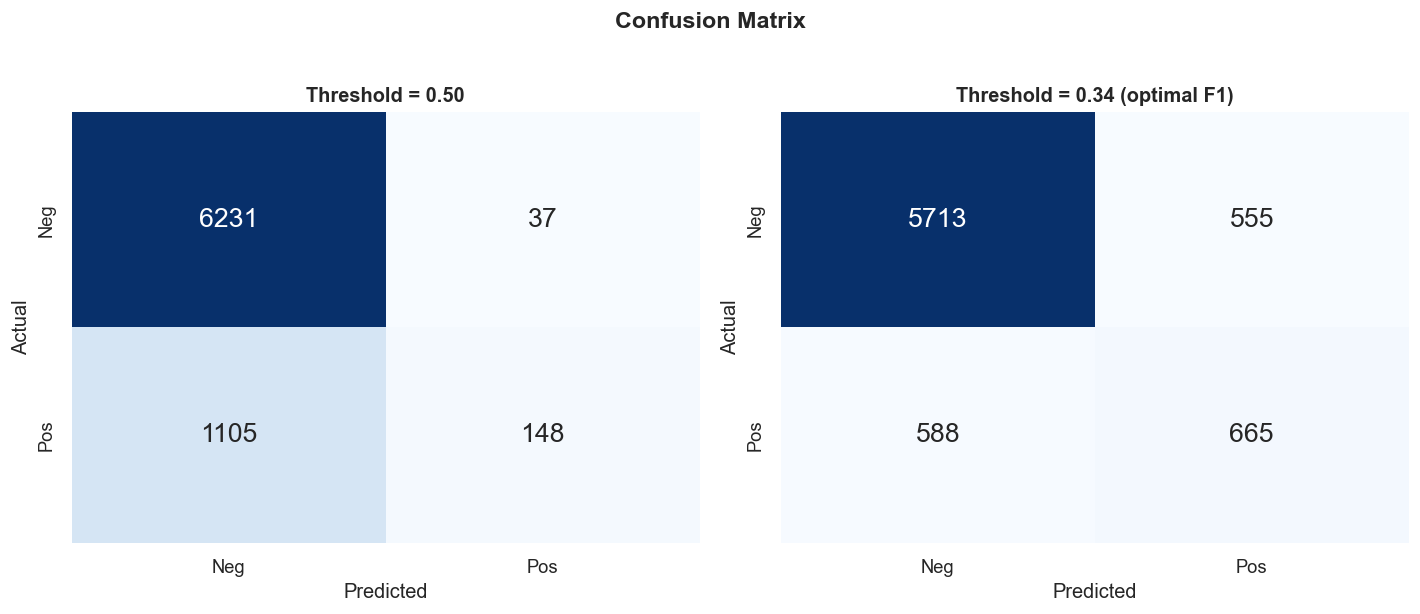
\includegraphics[width=0.9\linewidth]{img/roc_pr_approach4}
    \caption[ROC and Precision-Recall curves for the Approach 4 baseline]{ROC and Precision-Recall curves for the Approach~4 baseline
    classifier on the Group~A random-split test set.}
    \label{fig:results_roc_pr_baseline}
\end{figure}

\begin{figure}[htbp]
    \centering
    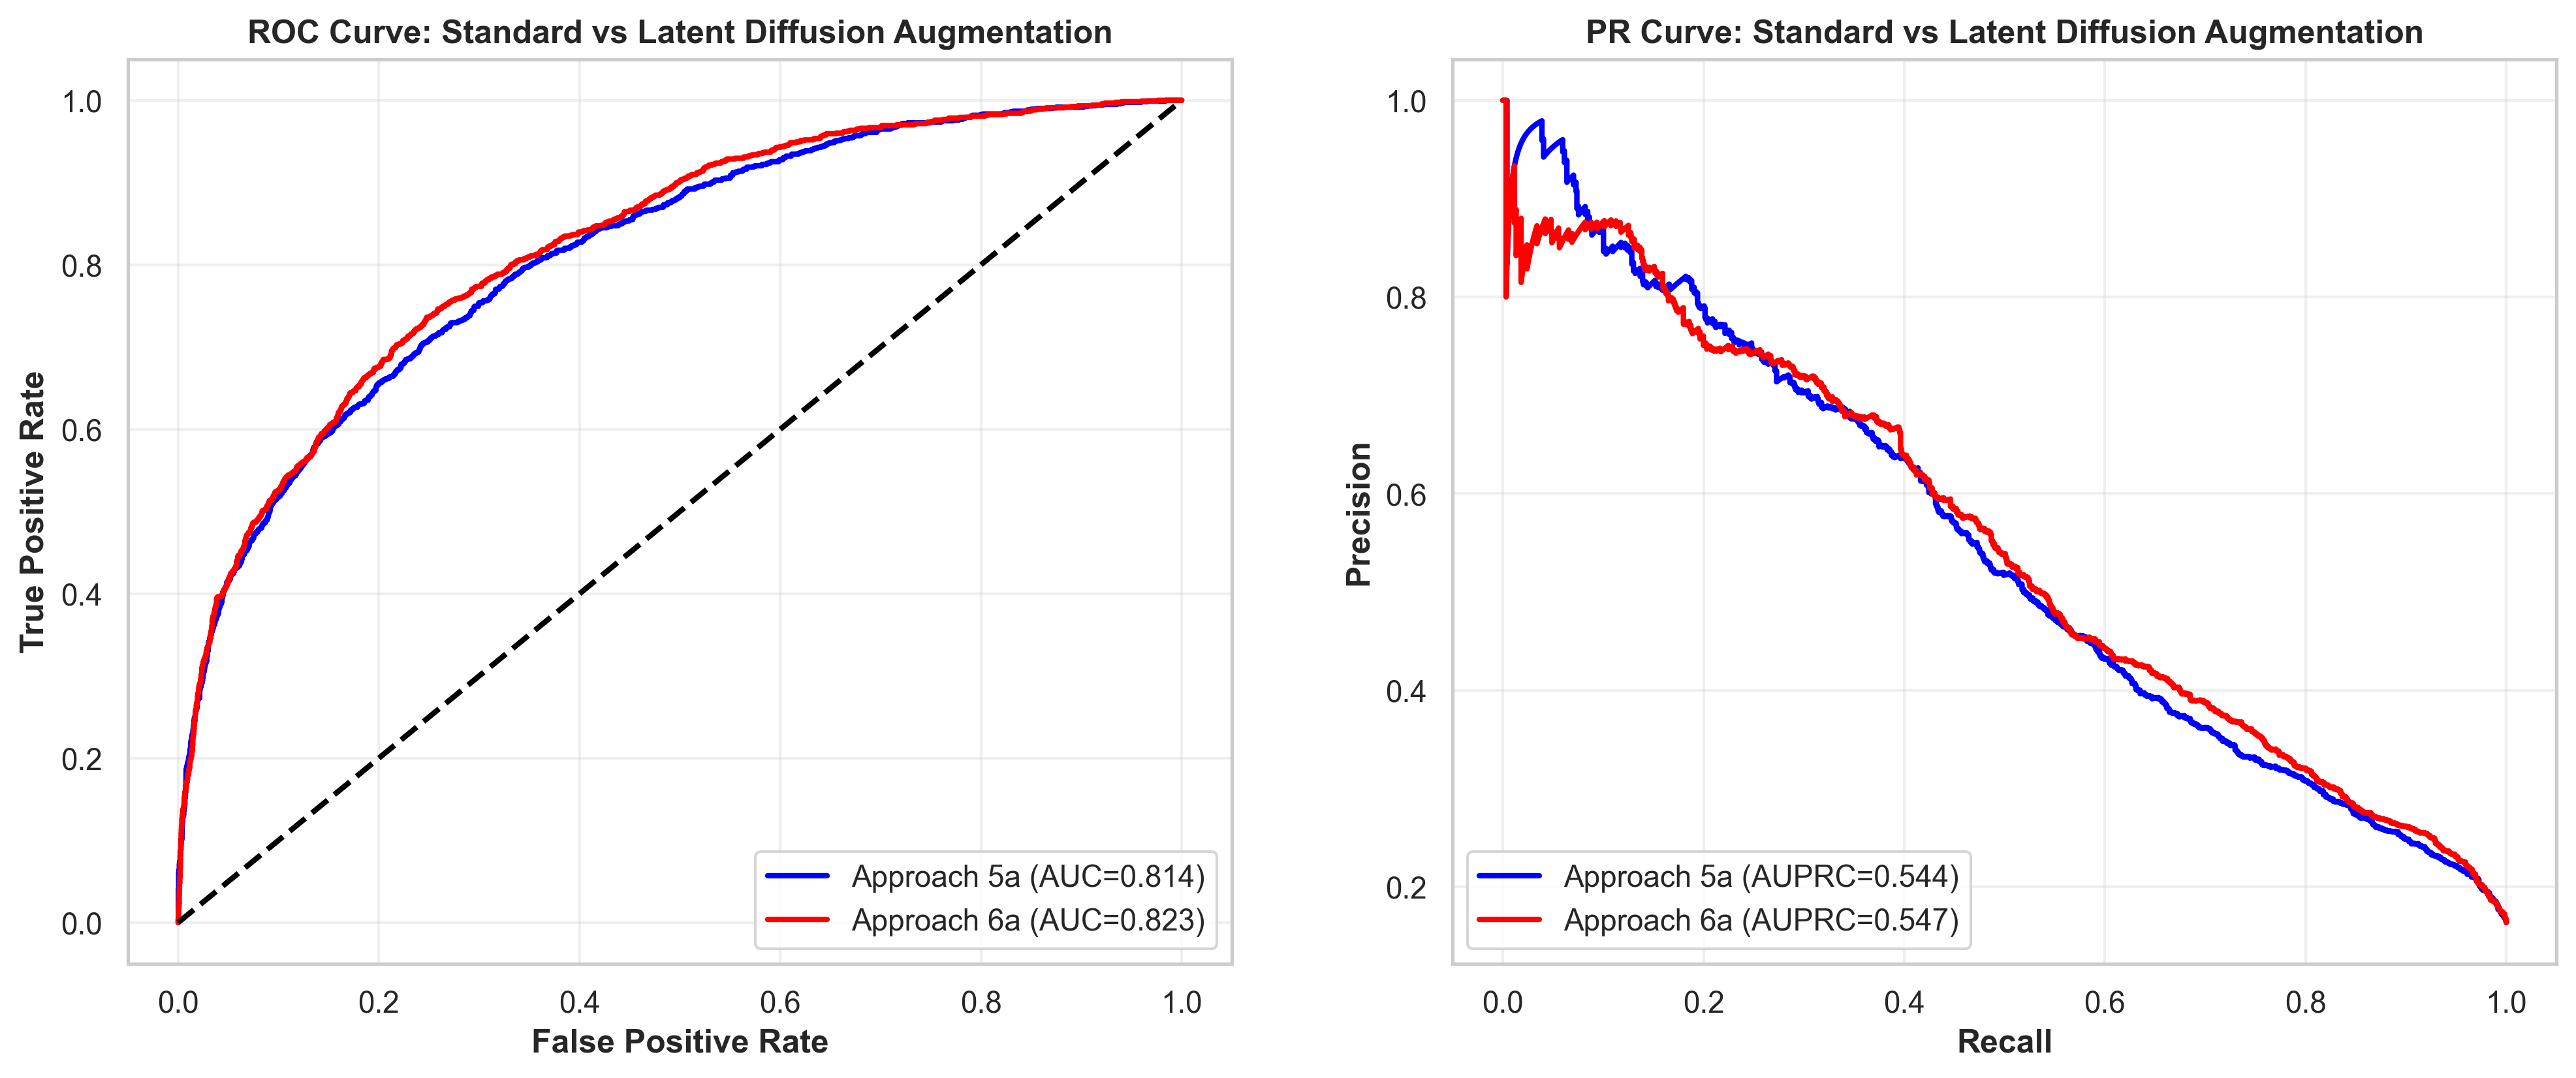
\includegraphics[width=0.9\linewidth]{img/comparison_5_vs_6_roc_pr}
    \caption[ROC and Precision-Recall curves: DDPM vs.\ LDM augmentation]{Comparison of ROC and Precision-Recall curves between DDPM
    (Approach~5) and LDM (Approach~6) augmentation strategies on the Group~A
    random-split test set.}
    \label{fig:results_comparison_roc_pr}
\end{figure}

\subsection{Group B: SaMi-Trop-Only Evaluation (Approach 10)}\label{sec:results_groupB}

Approach~10 (McSharry PINN) constitutes Group~B. Its only confirmed metrics are
the in-distribution validation scores on the CODE-15\% validation split at
epoch~40: validation AUROC $0.8273$ and validation AUPRC $0.4949$. These are
summarised in Table~\ref{tab:groupB}.

\begin{table}[htbp]
\centering
\caption[Group B result for Approach 10 (McSharry PINN)]{Group~B result (Approach~10, McSharry PINN). Only CODE-15\% validation
metrics are confirmed. The designated test set was SaMi-Trop ($1{,}631$
recordings, $100\%$ positive), a single-class set for which AUROC and the
Challenge Score are mathematically undefined.}
\label{tab:groupB}
\begin{tabular}{l c c}
\hline
\textbf{Metric} & \textbf{Value} & \textbf{Split} \\
\hline
AUROC & 0.8273 & CODE-15\% validation \\
AUPRC & 0.4949 & CODE-15\% validation \\
\hline
\end{tabular}
\end{table}

The test set assigned to Approach~10 was SaMi-Trop, comprising $1{,}631$
recordings that are all Chagas positive. Because this set contains a single
class, both AUROC and the Challenge Score are mathematically undefined: AUROC
requires both positive and negative examples, and TPR@5\% FPR cannot be computed
without negatives. The committed notebook of record also contains no
test-evaluation cell, so no out-of-distribution (OOD) sensitivity value is
reported here. The interpretation of Approach~10 as a potential ``Clever-Hans''
model is deferred to the Discussion (Chapter~\ref{chap:conclusions}) as a
hypothesis, grounded in the combination of a high in-distribution validation
AUROC and a single-class OOD test set rather than in a measured OOD value. As
architectural evidence for that hypothesis, the McSharry feature-importance
analysis in Figure~\ref{fig:results_feature_importance} shows that the baseline
offset parameter $z_0$ receives disproportionate weight; this analysis derives
from logistic regression fitted to ODE parameters extracted on the validation
set, and should be read as an architectural indication rather than a test-set
result.

\begin{figure}[htbp]
    \centering
    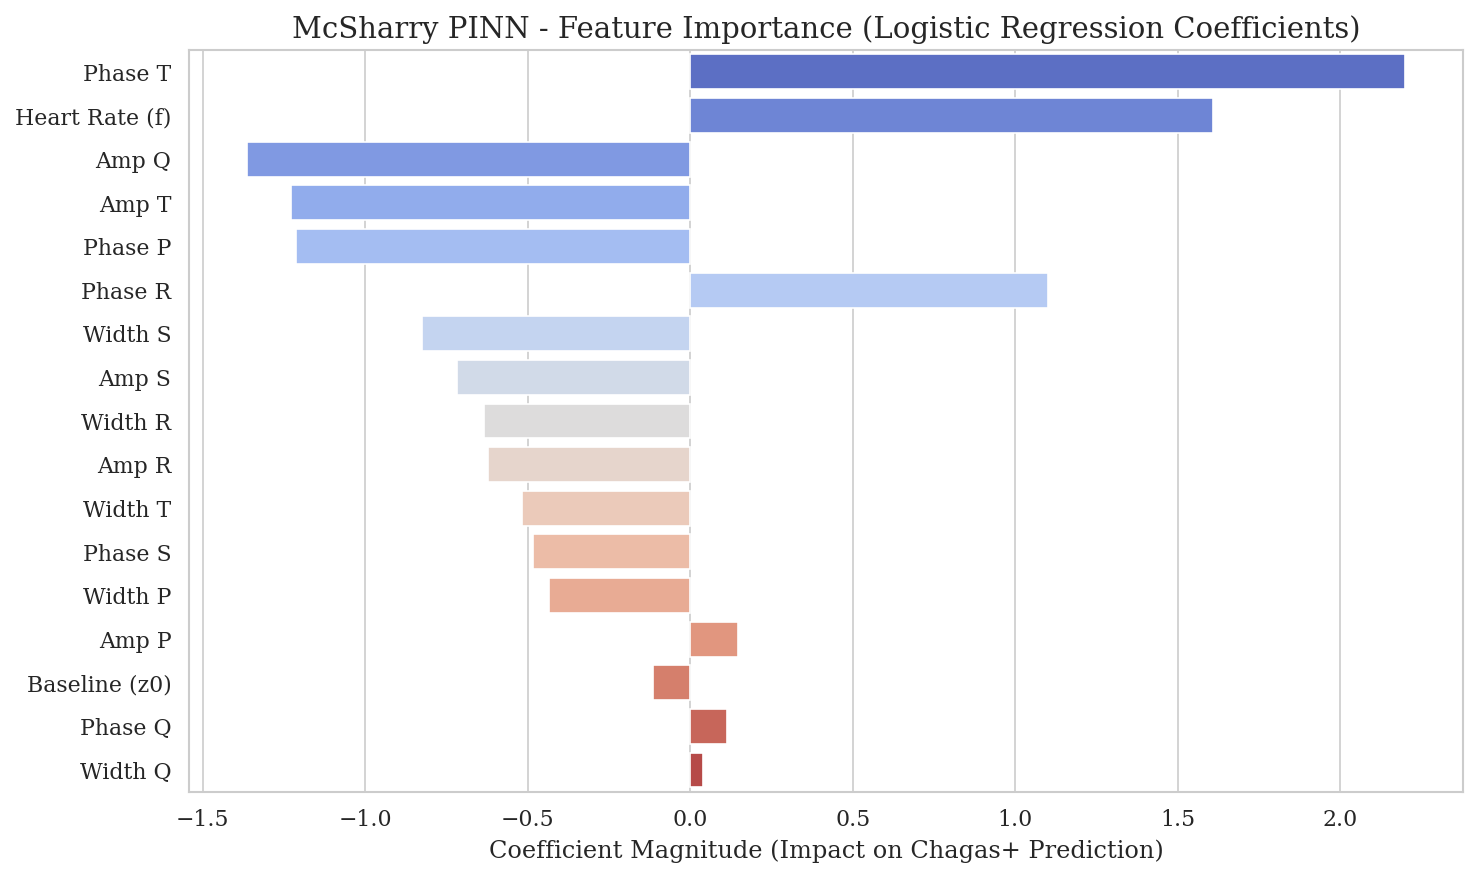
\includegraphics[width=0.9\linewidth]{img/pinn_feature_importance}
    \caption[Feature importance of the McSharry ODE parameters (Approach 10)]{Feature importance of the McSharry ODE parameters, derived from
    logistic regression coefficients on parameters extracted from the
    validation set. The baseline offset $z_0$ receives disproportionate weight,
    offered here as architectural evidence for the Approach~10 Clever-Hans
    hypothesis discussed in Chapter~\ref{chap:conclusions}.}
    \label{fig:results_feature_importance}
\end{figure}

\subsection{Group C: Isolated OOD Evaluation (Approaches 11, 12, 14, 15)}\label{sec:results_groupC}

Group~C comprises the phenomenological autoencoder and the
foundation-model / self-supervised approaches. These models were evaluated on a
CODE-15\% held-out test set of approximately $7{,}129$--$7{,}134$ samples at
roughly $13.8\%$ prevalence, with SaMi-Trop held fully isolated as an
out-of-distribution test set. Bootstrap $95\%$ confidence intervals were
computed from $1{,}000$ resamples (seed~42). The results, including the
SaMi-Trop OOD sensitivity at the operating threshold, appear in
Table~\ref{tab:groupC}.

\begin{table}[htbp]
\centering
\caption[Group C results for Approaches 11, 12, 14, 15]{Group~C results (Approaches 11, 12, 14, 15) on the CODE-15\% held-out
test set ($\approx 7{,}129$--$7{,}134$ samples, $\approx 13.8\%$ prevalence).
SaMi-Trop was held fully isolated as an out-of-distribution (OOD) test set.
Bootstrap $95\%$ confidence intervals were computed from $1{,}000$ resamples
(seed~42) for Approaches~11, 12, and~15. The Challenge Score is TPR@5\% FPR. The
final column gives SaMi-Trop OOD sensitivity at the stated operating threshold.
Approaches~13 and~16 produced no results (see Section~\ref{sec:results_incomplete}).}
\label{tab:groupC}
\footnotesize
\begin{tabular}{@{}c p{2.4cm} p{2.1cm} p{2.1cm} p{2.1cm} p{2.3cm}@{}}
\hline
\textbf{Approach No.} & \textbf{Approach} & \textbf{AUROC (95\% CI)} & \textbf{AUPRC (95\% CI)} & \textbf{TPR@5\% (95\% CI)} & \textbf{OOD sens.\ @ thr.} \\
\hline
11 & McSharry autoencoder         & 0.7710 \newline [0.7555--0.7873] & 0.4004 \newline [0.3711--0.4338] & 0.2100 \newline [0.1936--0.2308] & 0.1312 @0.5 \newline (0.9945 @0.1) \\
12 & DeepECG-SSL fine-tune        & 0.8593 \newline [0.8484--0.8716] & 0.5813 \newline [0.5462--0.6086] & 0.2869 \newline [0.2688--0.3049] & 0.0000 \\
14 & Hybrid ECGFounder + PINN     & $0.8288^{\dagger}$               & $0.4767^{\dagger}$               & $-^{\dagger}$                    & 0.4096 @0.487 \\
15 & DeepECG-SSL + temporal attn. & 0.8351 \newline [0.8240--0.8495] & 0.5119 \newline [0.4778--0.5458] & 0.2602 \newline [0.2418--0.2803] & 0.2949 @0.5 \\
\hline
\end{tabular}

\vspace{2pt}
{\footnotesize $^{\dagger}$ Point estimates from the executed notebook cell
(\texttt{approach14\_hybrid\_fm\_pinn.ipynb}, cell~10). Bootstrap confidence
intervals were not computed for Approach~14: regenerating its predictions
requires inference through the ECGFounder foundation-model encoder, whose
CPU-only cost in the available hardware environment ($\approx 4$~s per recording,
no GPU/MPS) was prohibitive. The Challenge Score (TPR@5\%) was not reported for
this approach in the source notebook.}
\end{table}

\begin{figure}[htbp]
    \centering
    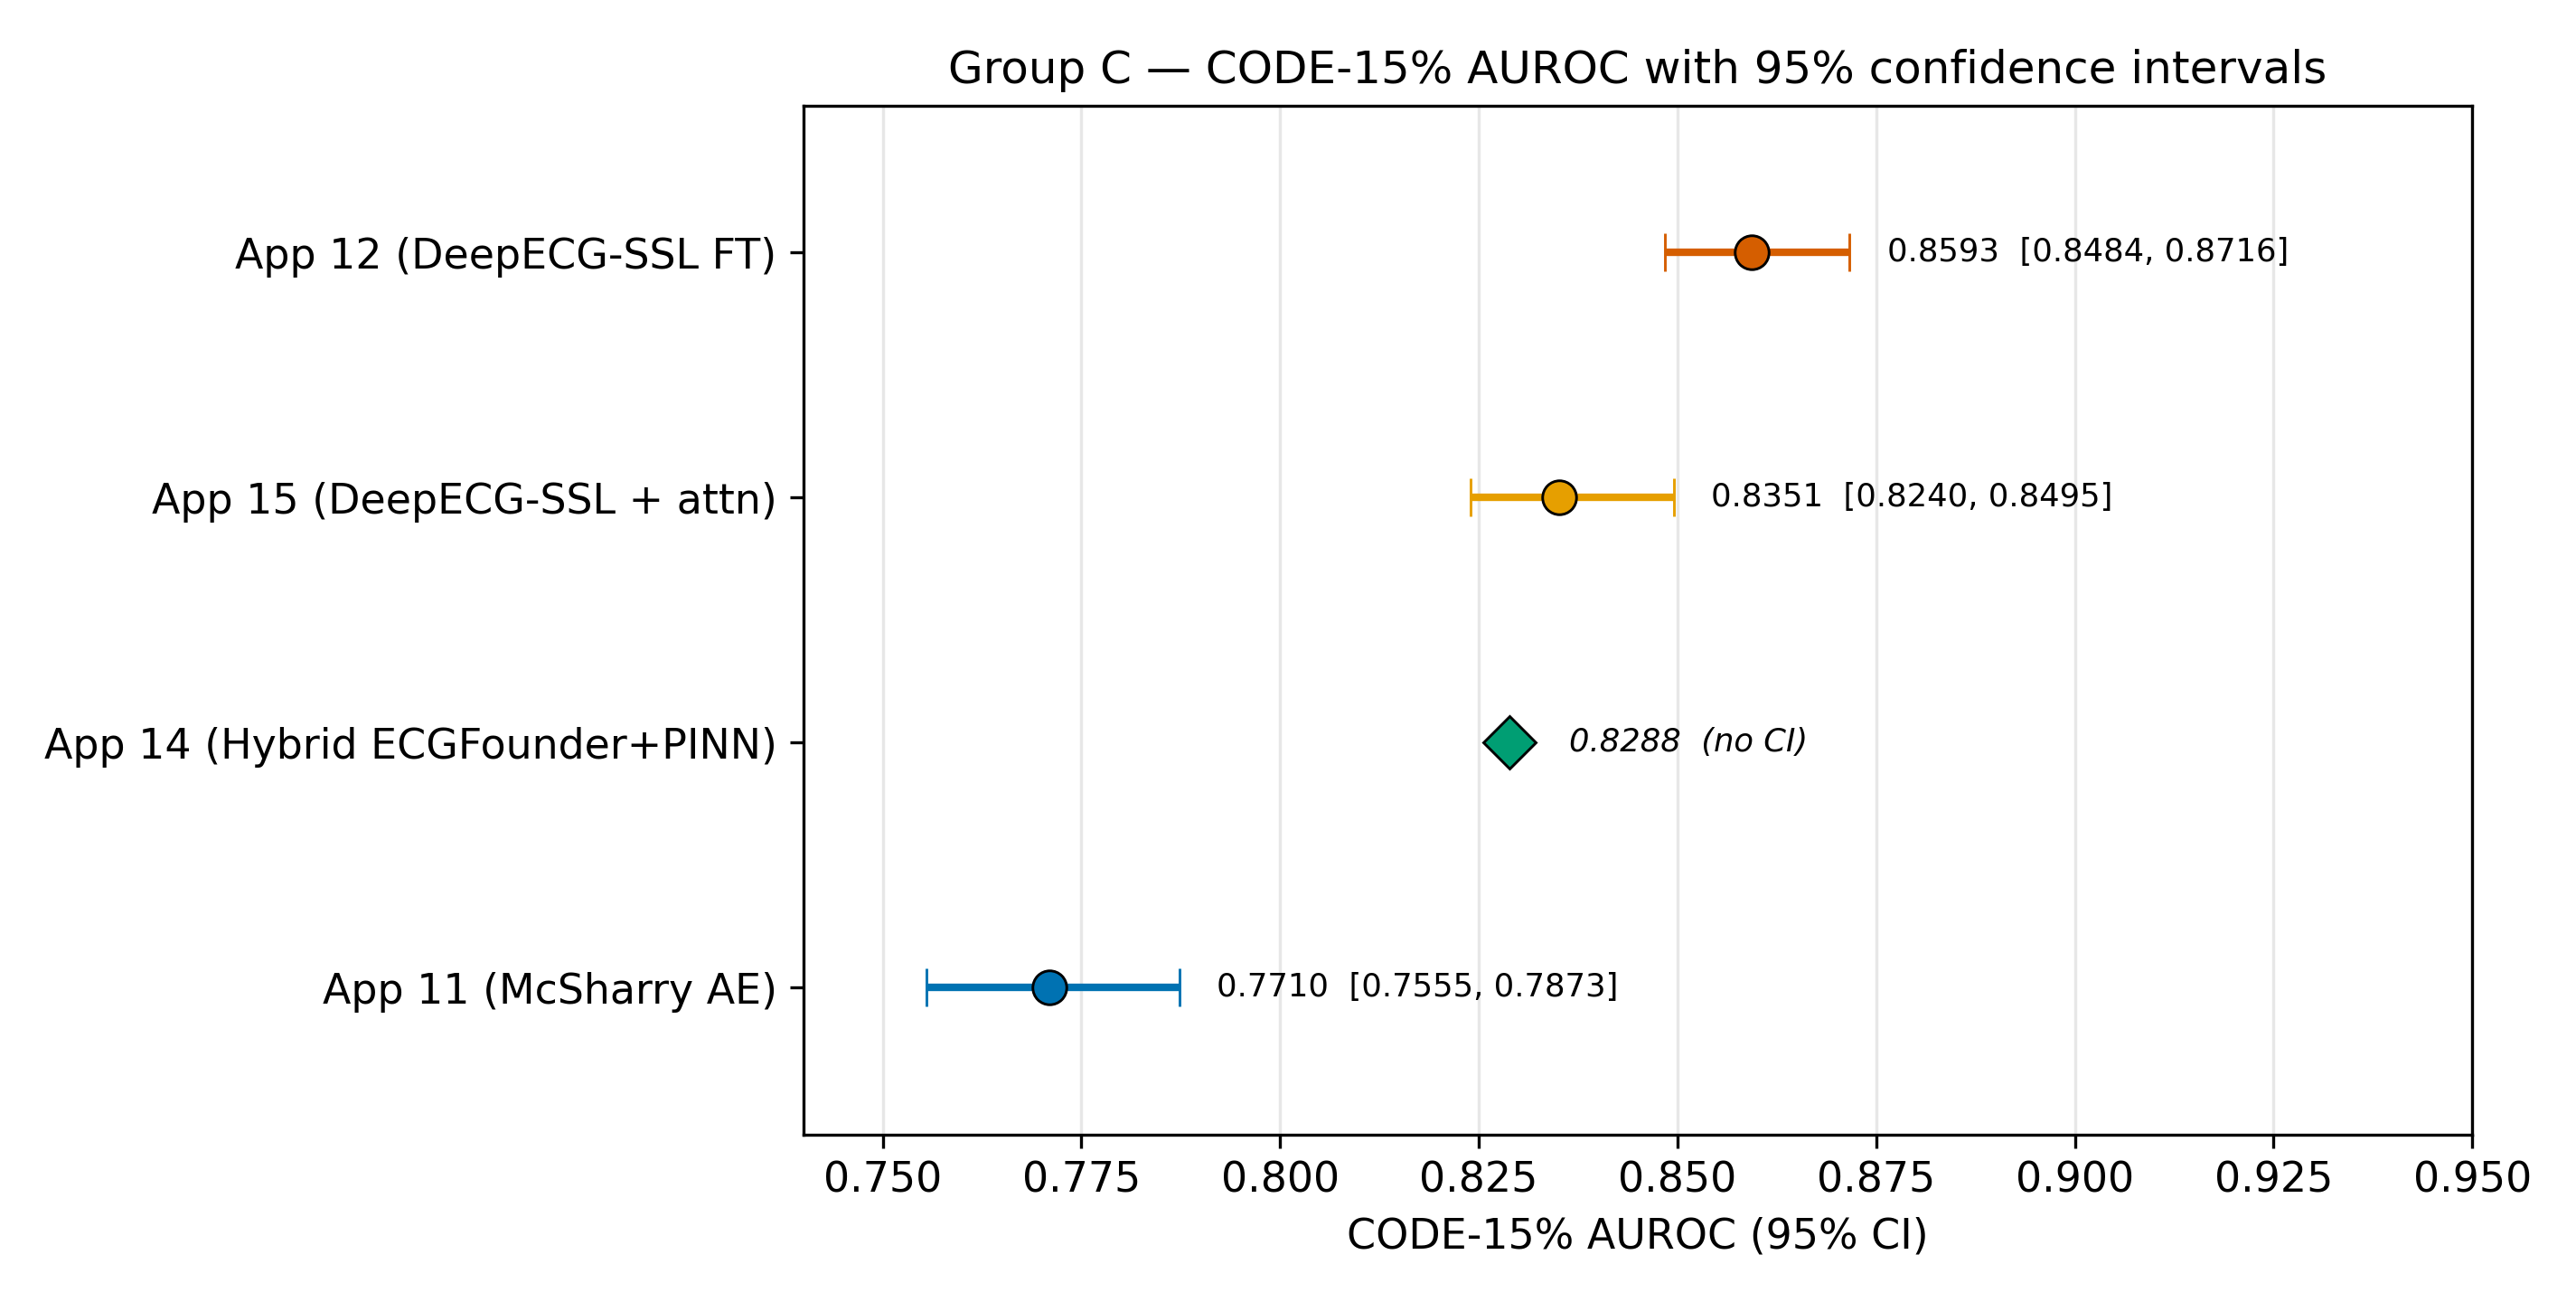
\includegraphics[width=0.85\linewidth]{img/groupc_forest}
    \caption[CODE-15\% held-out AUROC forest plot for Group-C approaches]{CODE-15\% held-out AUROC of the Group-C approaches with bootstrap
    $95\%$ confidence intervals (Approaches~11, 12, and~15). Approach~14 is shown
    as a point without an interval, as its bootstrap CI could not be computed
    (see the note to Table~\ref{tab:groupC}).}
    \label{fig:groupc_forest}
\end{figure}

Within Group~C, Approach~12 (DeepECG-SSL fine-tune) attained the highest
CODE-15\% test AUROC at $0.8593$ ($[0.8484, 0.8716]$) and the highest Challenge
Score at $0.2869$, yet its SaMi-Trop OOD sensitivity at the default threshold
was $0.0000$. The AUROC ranking and its confidence intervals are summarized in
Figure~\ref{fig:groupc_forest}. Approach~15 (DeepECG-SSL with temporal attention) reached an AUROC
of $0.8351$ and recovered $0.2949$ of SaMi-Trop positives at threshold $0.5$.
Approach~14 (hybrid ECGFounder + McSharry PINN) achieved an AUROC of $0.8288$
and the highest OOD sensitivity in Group~C, $0.4096$, at threshold $0.487$ (mean
predicted probability $0.4511$); bootstrap confidence intervals could not be
computed for this approach owing to the prohibitive cost of foundation-model
inference in the available CPU-only environment, as detailed in the note to
Table~\ref{tab:groupC}. Approach~11
(McSharry autoencoder) had the lowest in-distribution AUROC at $0.7710$, but its
OOD behavior is examined in detail in Section~\ref{sec:results_app11_sweep}.

\subsection{Approach 11 Threshold Sweep}\label{sec:results_app11_sweep}

The OOD behavior of Approach~11 depends strongly on the decision threshold. On
the isolated SaMi-Trop set, the mean predicted score was $0.3331$. At the default
threshold of $0.5$, the sensitivity was only $0.1312$ ($214$ of $1{,}631$
positives recovered). Lowering the threshold to $0.1$ raised the sensitivity to
$0.9945$ ($1{,}622$ of $1{,}631$ positives recovered). The full sensitivity
profile as a function of threshold is shown in
Figure~\ref{fig:app11_threshold_sweep}.

\begin{figure}[htbp]
    \centering
    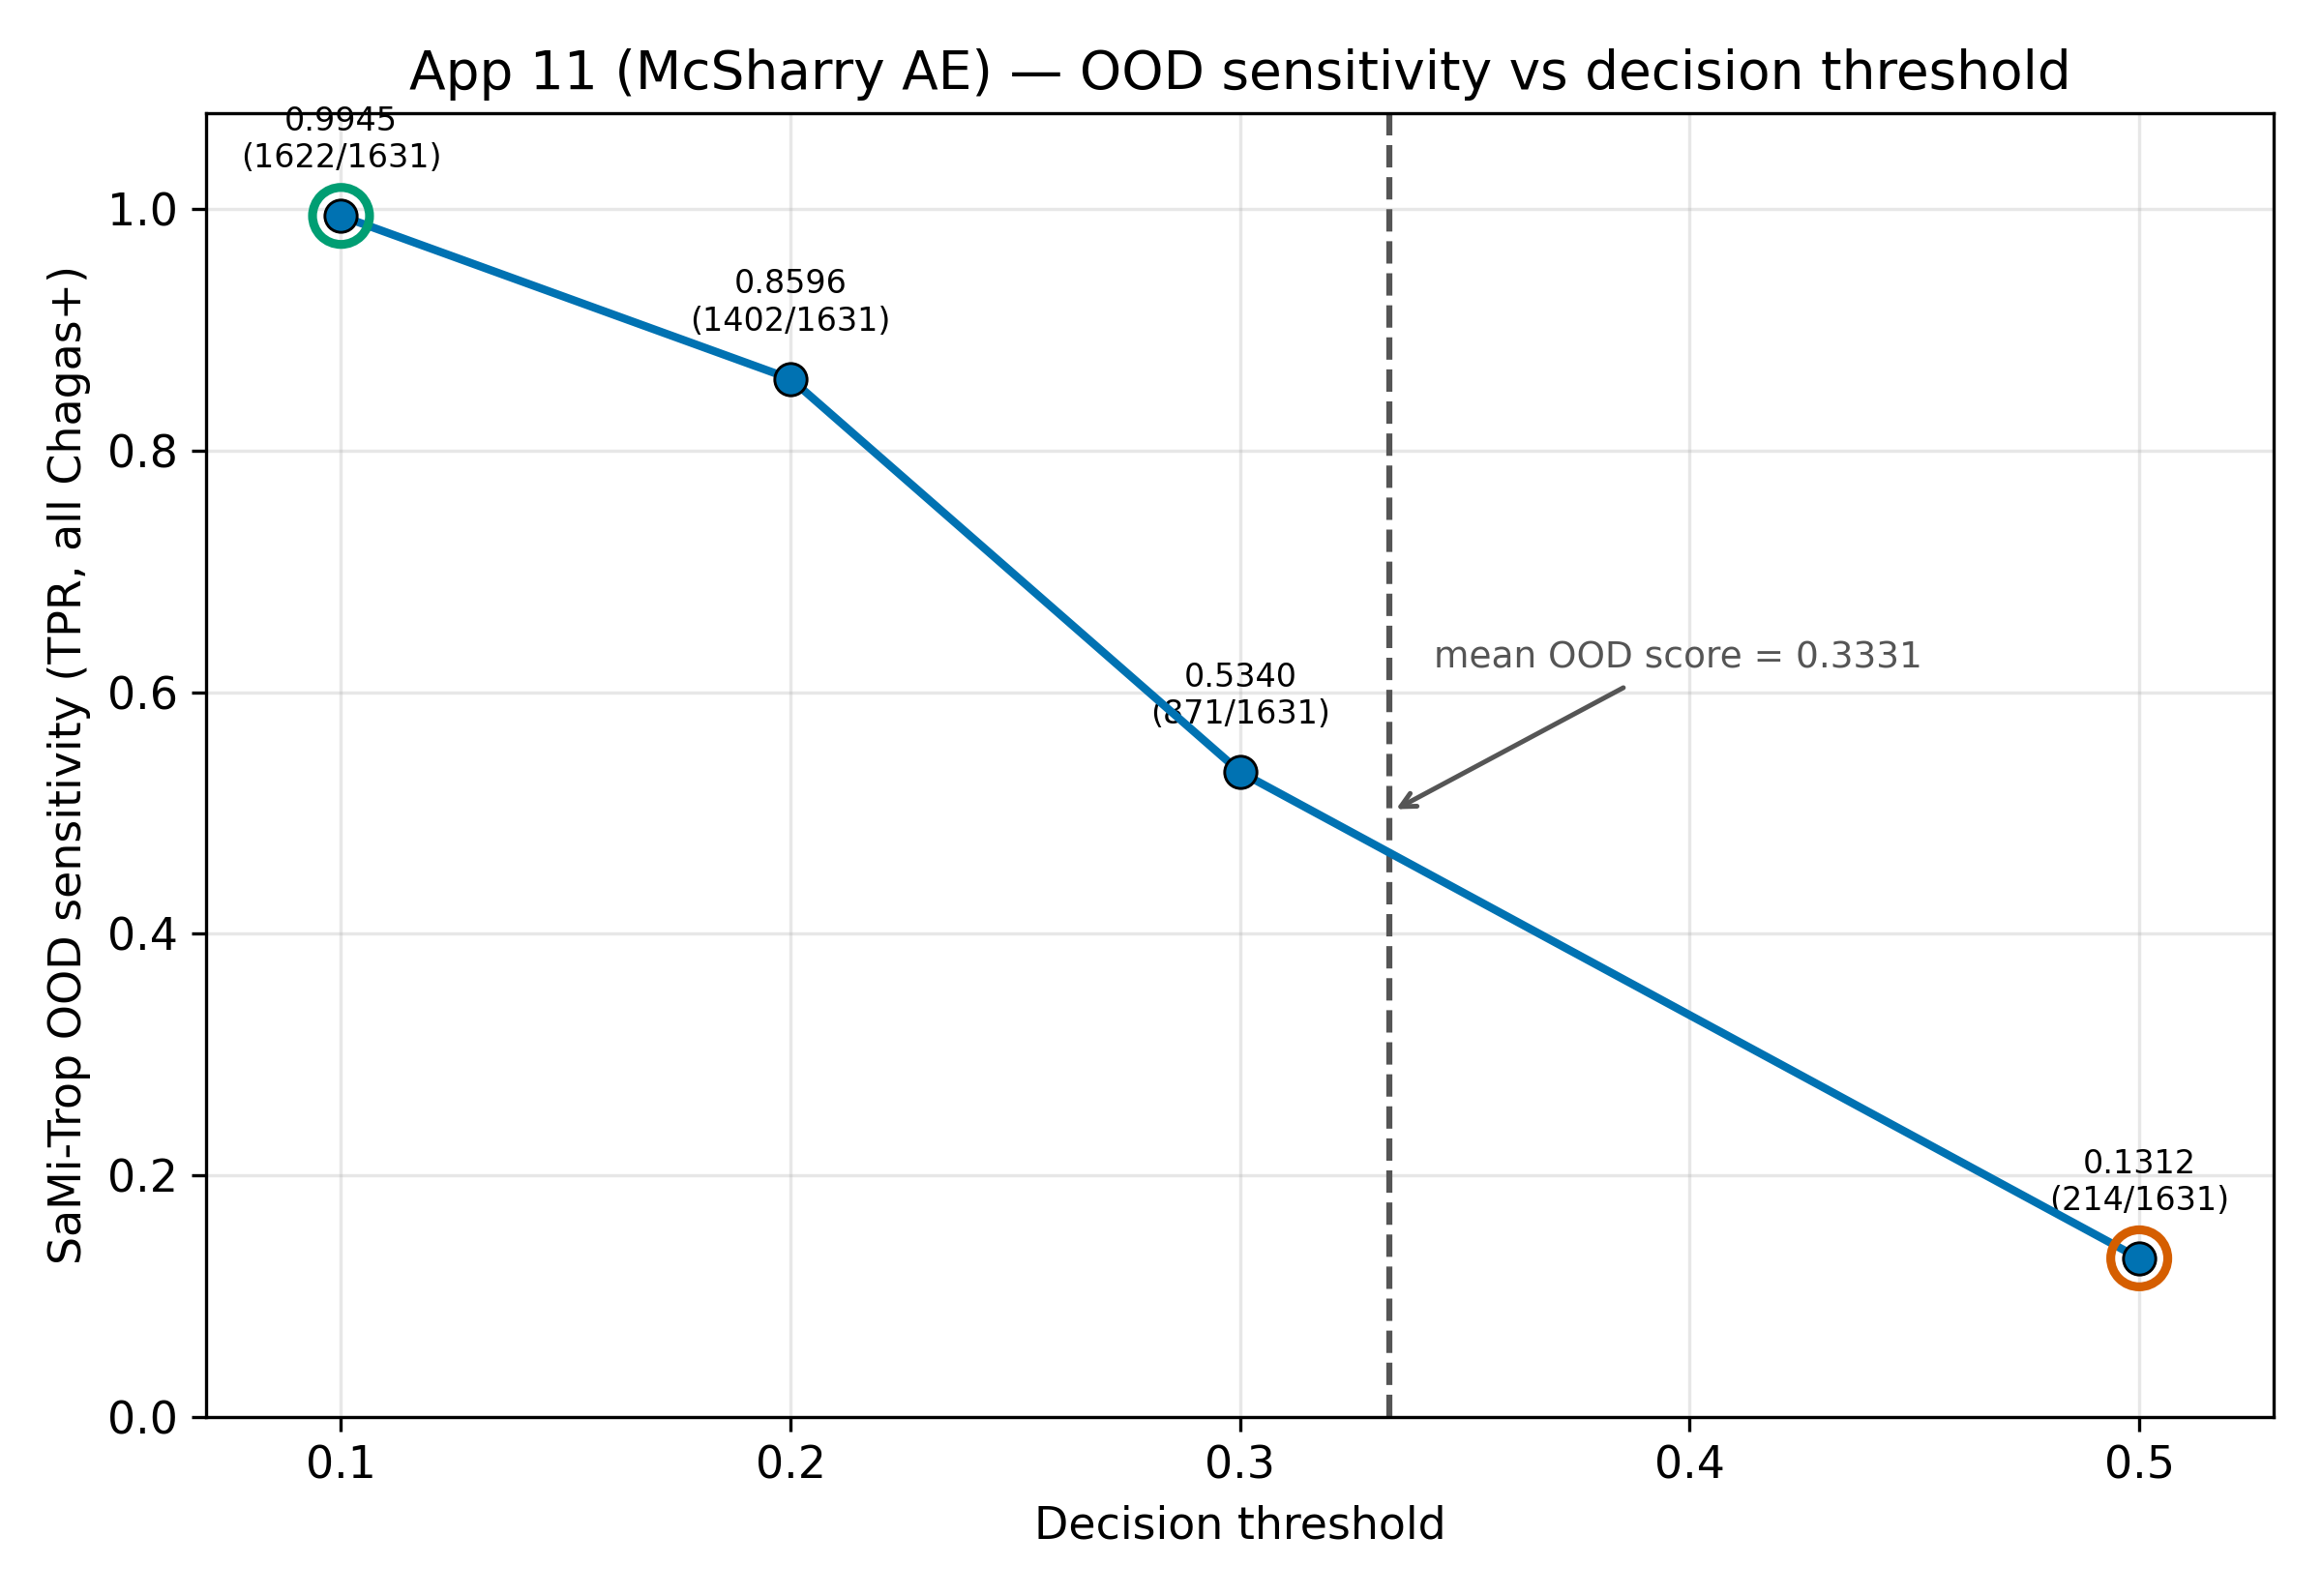
\includegraphics[width=0.9\linewidth]{img/app11_threshold_sweep}
    \caption[Approach 11 SaMi-Trop OOD sensitivity vs.\ decision threshold]{SaMi-Trop out-of-distribution sensitivity of Approach~11 as a
    function of the decision threshold. Sensitivity is $0.9945$ at threshold
    $0.1$ and falls to $0.1312$ at the default threshold of $0.5$; the mean
    predicted OOD score is $0.3331$.}
    \label{fig:app11_threshold_sweep}
\end{figure}

This pattern indicates that the discriminative signal for the SaMi-Trop
population is present in the Approach~11 scores but is concentrated below the
default $0.5$ cutoff. The threshold sweep thus sets up a finding examined in the
Discussion (Chapter~\ref{chap:conclusions}): a single threshold adjustment,
rather than retraining, recovers most of the OOD positives.

\subsection{Incomplete Experiments (Approaches 13 and 16)}\label{sec:results_incomplete}

Two experiments did not reach completion and therefore report no quantitative
results.

Approach~13 (ECGFounder + XGBoost) was only partially executed. The committed
notebook ran cells~1 through~3, which load the foundation model, but the
subsequent feature-extraction, XGBoost-training, and evaluation cells never ran,
and no artifacts were written to disk. Consequently, no AUROC, AUPRC, or
feature-attribution results exist for this approach. It stands as a documented
attempt and a candidate for future work.

Approach~16 (cross-domain PTB-XL) was never executed for inference because the required
model weights were missing. Only the experimental design was realized. Any
false-positive-rate figures previously circulated for this approach are invalid
and are not reported here. Like Approach~13, it remains a documented attempt and
a direction for future work.

\chapter{Discussion and Conclusions}
\label{chap:conclusions}
\label{chap:discussion}

\section{The Central Finding: AUROC Misranks Models for the Clinical OOD Task}
\label{sec:central_finding}

The argument is organized around a single empirical observation that contradicts what the field assumes: the metric used to rank models on internal leaderboards, the area under the receiver operating characteristic curve (AUROC), does not predict which model is useful for the real clinical task, namely detecting disease in an out-of-distribution (OOD) patient population. This observation leads to three further developments: a taxonomy that separates two qualitatively different OOD failure modes, an OOD-sensitivity ranking that turns out to invert the AUROC ranking, and a comparison between physics-based and phenomenological inductive biases. Throughout, the inviolable rule established in Chapter~\ref{chap:research} is observed: metrics belonging to different evaluation groups (A, B, and C) are never compared as if they were commensurable.

The defining result of this thesis is a contrast between two Group-C models evaluated on the same held-out CODE-15\% set and the same isolated SaMi-Trop OOD cohort.

Approach~12, the fine-tuned DeepECG-SSL model, attains the highest CODE-15\% held-out AUROC of any approach in the thesis: $0.8593$ (95\% CI $[0.8484,\,0.8716]$). On the conventional leaderboard it is unambiguously the best discriminator. Yet when this same model is applied at its default decision threshold to the SaMi-Trop cohort, a population it never saw during training, it identifies none of the positive patients: its OOD sensitivity is exactly $0.0000$. Because the SaMi-Trop test set contains a single class, AUROC is undefined there, so the in-distribution figure of merit cannot even be computed on the population that matters.

Approach~11, the McSharry autoencoder, presents the mirror image. It has the \emph{lowest} CODE-15\% AUROC in Group~C, $0.7710$ (95\% CI $[0.7555,\,0.7873]$). By the leaderboard it is the weakest of the four Group-C models. On the SaMi-Trop cohort, however, the disease signal is plainly present: the mean predicted OOD score is $0.3331$, and a single adjustment of the decision threshold from the default $0.5$ to $0.1$ recovers $99.45\%$ of the cohort (sensitivity $0.9945$, $1622/1631$).

\begin{figure}[htbp]
    \centering
    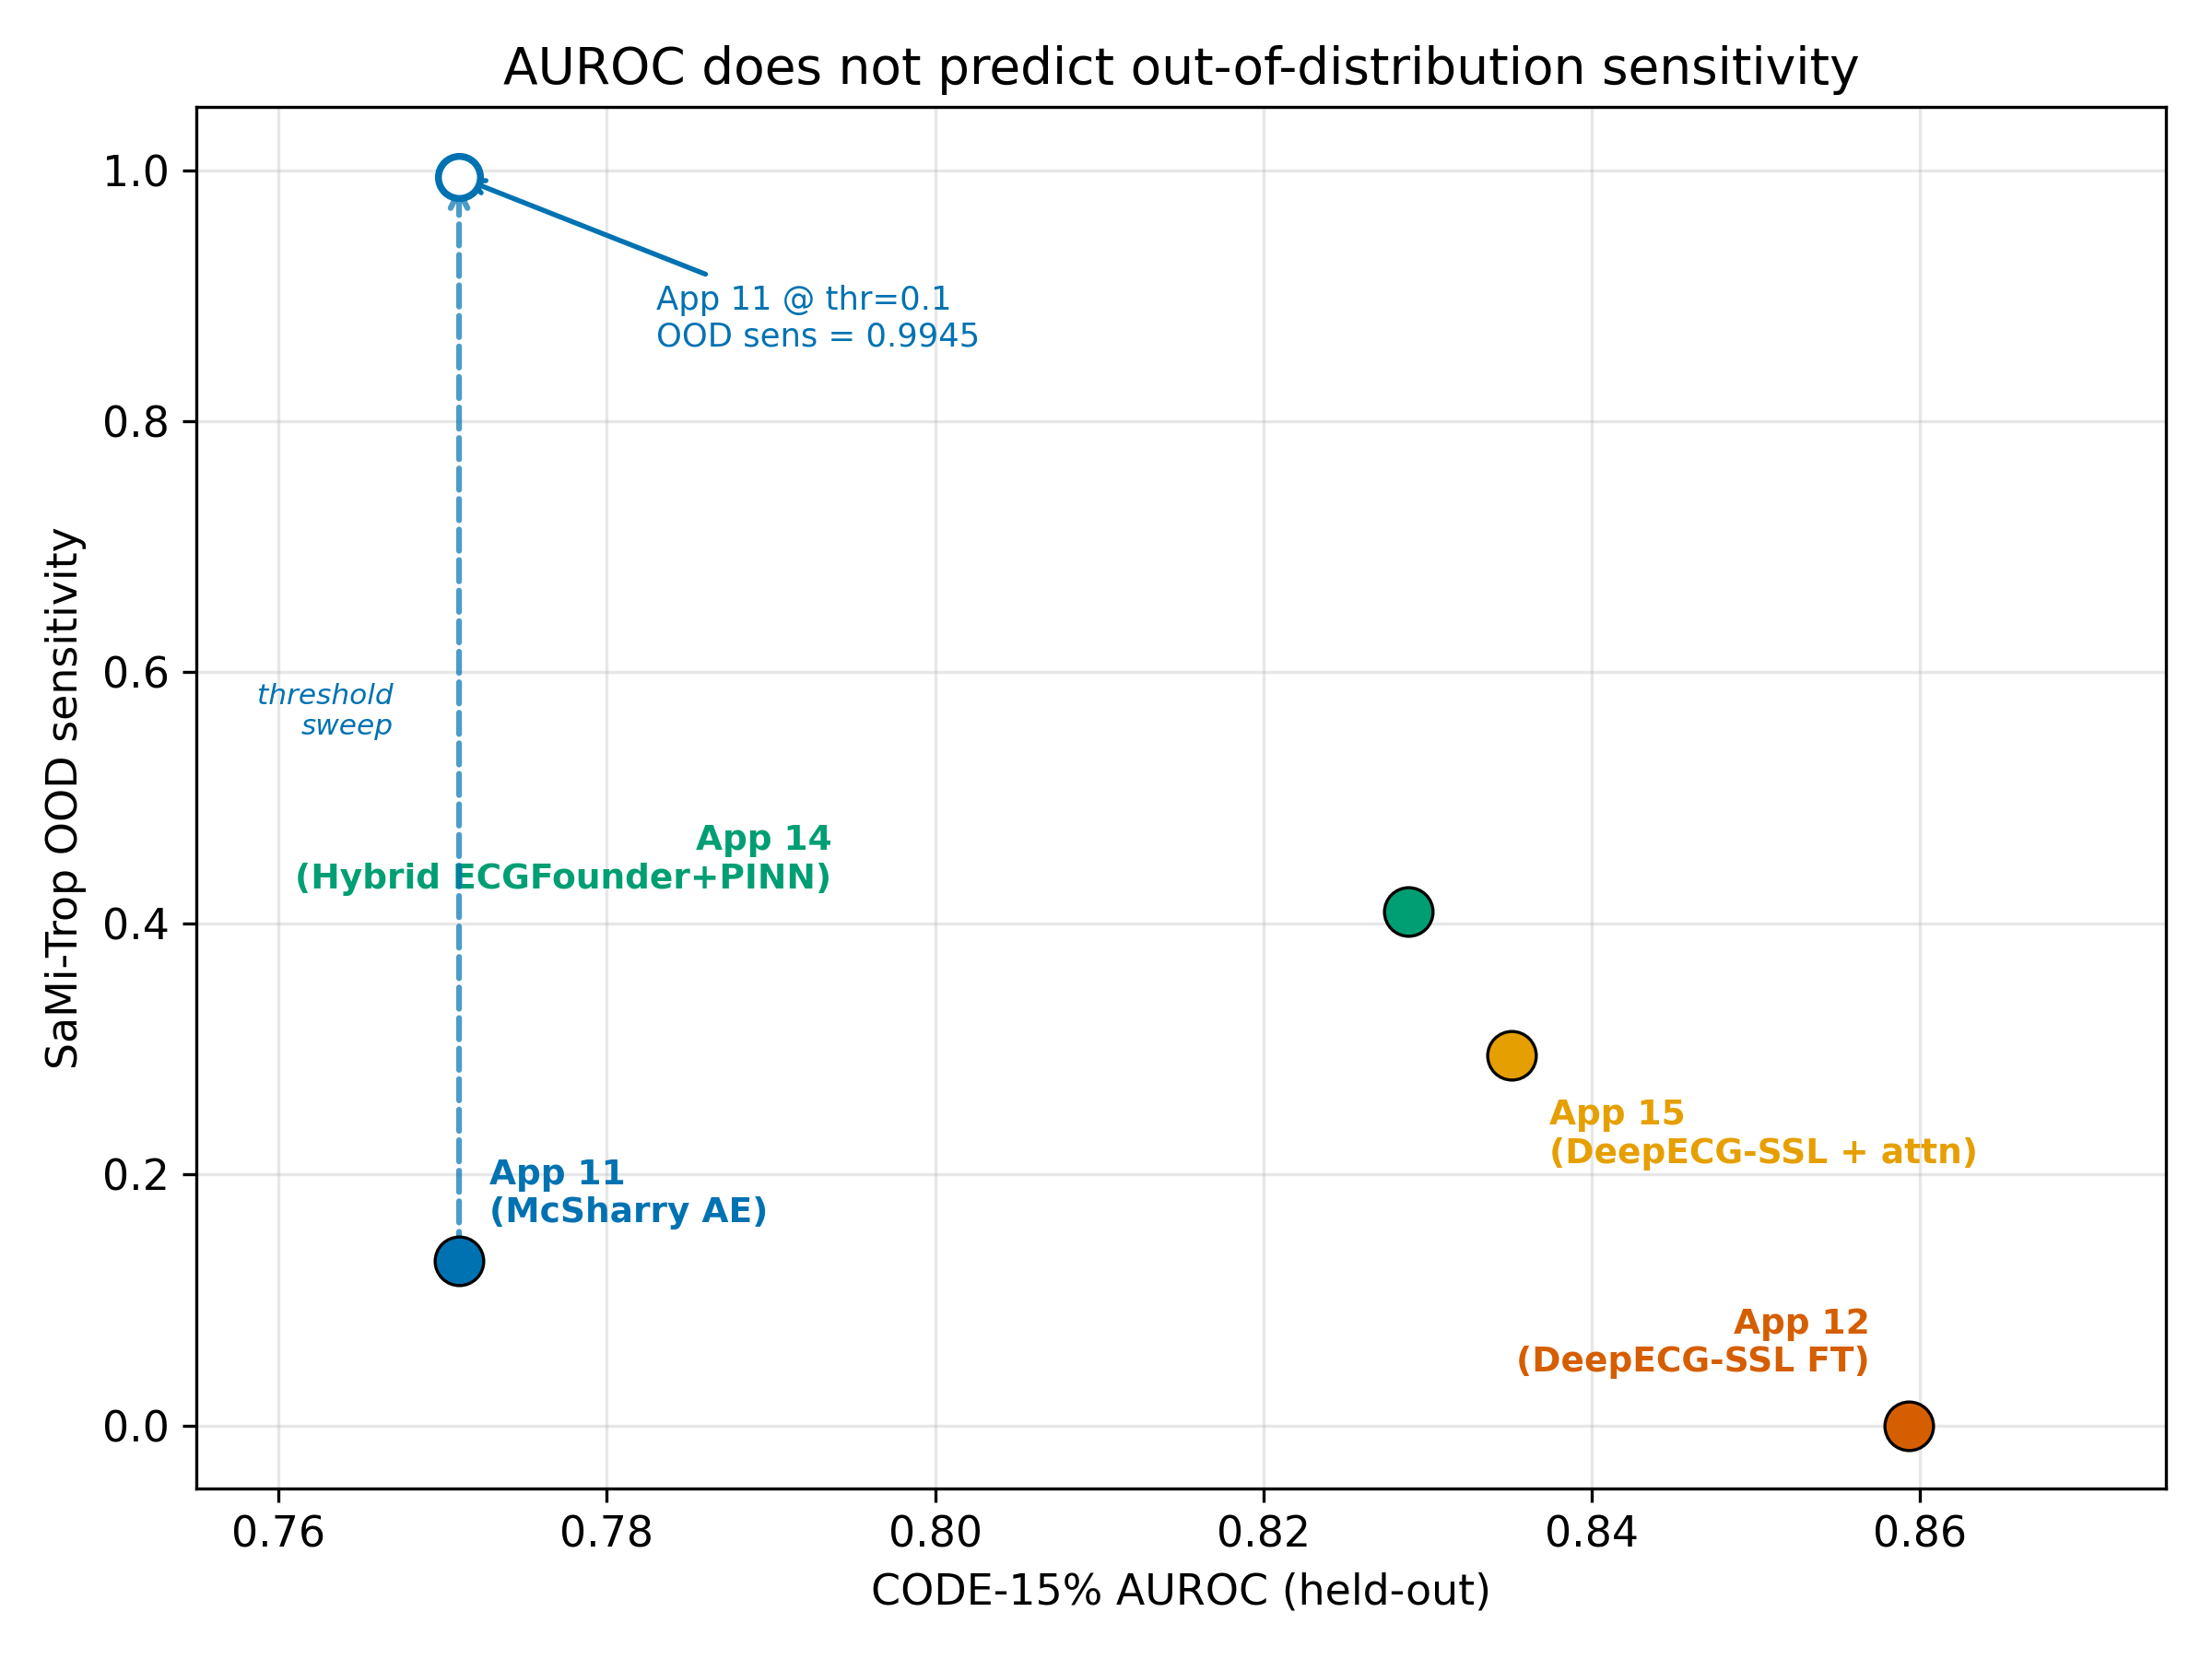
\includegraphics[width=0.85\linewidth]{img/auroc_vs_ood}
    \caption[OOD sensitivity vs.\ in-distribution AUROC for Group-C approaches]{Out-of-distribution sensitivity on the SaMi-Trop cohort as a
    function of in-distribution AUROC on CODE-15\% for the four Group-C
    approaches. A high AUROC does not translate into out-of-distribution
    sensitivity: Approach~12 attains the highest AUROC yet zero OOD sensitivity
    at its default threshold, whereas Approach~11 detects $99.45\%$ of the cohort
    once its threshold is lowered to $0.1$ (dashed arrow). Selecting a model by
    AUROC alone would deploy the worst performer for the clinical screening task.}
    \label{fig:auroc_vs_ood}
\end{figure}

Placed side by side (Figure~\ref{fig:auroc_vs_ood}), these two facts establish the central claim. A threshold-independent, in-distribution discriminative metric does not predict OOD screening sensitivity. It also ranks the two models in the wrong order for the clinical task: the model that the AUROC leaderboard crowns (Approach~12) is the one that, deployed as-is, would miss every Chagas-positive patient in the endemic cohort, whereas the model the leaderboard relegates to last place (Approach~11) is the one whose latent signal can be turned into near-complete OOD recall with a single threshold move. A practitioner who selected a model by AUROC alone would deploy the wrong system. This is the answer to RQ5, posed in Chapter~\ref{chap:introduction}: threshold-independent discriminative performance does \emph{not} rank models correctly for the real clinical out-of-distribution screening task.

The deeper reason is that AUROC rewards the \emph{separability} of scores within a fixed distribution while saying nothing about where those scores land relative to a deployed threshold once the distribution shifts. A model can rank in-distribution positives above in-distribution negatives very well (high AUROC) and still map an entire shifted population below its operating point (zero sensitivity at the default cutoff). For a screening instrument, whose entire value lies in catching cases under distribution shift, this is the failure that matters, and it is exactly the one AUROC is blind to.

\section{Two Distinct Out-of-Distribution Failure Modes}
\label{sec:failure_modes}

It would be a mistake to lump every OOD shortfall together. The results expose two qualitatively different failure modes, and conflating them would obscure the only one that admits a cheap remedy.

The first mode is a genuine \emph{Clever Hans} failure, and the term is reserved here for Approach~10, the McSharry phenomenological PINN, alone. Approach~10 achieves a strong in-distribution validation AUROC of $0.8273$ on CODE-15\% yet, the hypothesis holds, carries no transferable disease signal to a shifted population. This is a hypothesis, not a measured number: the committed notebook of record for Approach~10 contains no test-evaluation cell, so no SaMi-Trop sensitivity was actually recorded, and none is asserted here. The hypothesis is grounded instead in two structural facts. First, the model's parametrization is richly over-specified for the task: it exposes seventeen free phenomenological parameters, including a baseline-offset term $z_0$ that captures the recording's isoelectric line, an equipment- and acquisition-specific artifact rather than a marker of cardiac pathology~\cite{mcsharry2003dynamical}. A model with that many degrees of freedom can fit the validation distribution by leaning on such artifacts, in the manner of Clever Hans answering not the question asked but a spurious cue correlated with it~\cite{muller2019does}. Second, the OOD test set is single-class, which means a Clever-Hans model anchored to source-domain artifacts would have no opportunity to be corrected and every opportunity to fail silently. The claim about Approach~10 is therefore architectural and evidential, not a quantitative measurement.

The second mode is entirely different and is exemplified by Approach~11: a \emph{calibration} or \emph{threshold-shift} failure. Here the transferable disease signal is demonstrably present. The mean predicted OOD score on SaMi-Trop is $0.3331$, well above zero and concentrated in a region the model treats as mildly suspicious. The failure is not that the model cannot see the disease; it is that the default $0.5$ decision threshold sits above where the OOD scores accumulate, suppressing a signal the model has in fact extracted. Lowering the threshold to $0.1$ converts that latent signal into $99.45\%$ sensitivity. This is a miscalibration of the operating point under distribution shift, the kind of problem that post-hoc threshold or probability recalibration is designed to address~\cite{guo2017calibration}, and it is emphatically \emph{not} Clever Hans: there is real signal to recalibrate.

The distinction is practically decisive. A Clever Hans model cannot be rescued by moving a threshold, because no threshold separates a signal that was never learned; it requires a different inductive bias or a debiased training procedure. A threshold-shift failure, by contrast, is the cheapest defect in machine learning to repair: it needs a single scalar adjustment on a small calibration sample from the target population. Treating the two as one and the same would either condemn a recoverable model (Approach~11) or raise false hope for an unrecoverable one (Approach~10).

\section{Out-of-Distribution Sensitivity Ranking}
\label{sec:ood_ranking}

Ranking the Group-C models by their SaMi-Trop OOD sensitivity yields an order that inverts the AUROC ranking. By AUROC the order is Approach~12 ($0.8593$) $>$ Approach~15 ($0.8351$) $>$ Approach~14 ($0.8288$) $>$ Approach~11 ($0.7710$). By OOD sensitivity it becomes:

\begin{itemize}
    \item Approach~14 (hybrid ECGFounder + McSharry PINN): sensitivity $0.4096$ at threshold $0.487$, the highest OOD sensitivity in Group~C;
    \item Approach~15 (DeepECG-SSL + temporal attention): sensitivity $0.2949$ at threshold $0.5$ ($481/1631$);
    \item Approach~11 (McSharry autoencoder): sensitivity $0.1312$ at the default threshold $0.5$ ($214/1631$), rising to $0.9945$ at threshold $0.1$;
    \item Approach~12 (DeepECG-SSL fine-tune): sensitivity $0.0000$.
\end{itemize}

The inversion is near-total: the AUROC leader is the OOD laggard, and the AUROC laggard becomes the OOD leader once its threshold is set appropriately. Approach~14, which is only third by AUROC, reaches the highest OOD sensitivity even at a near-default threshold, suggesting that its hybrid construction, a foundation-model backbone fused with physics-derived parameters, keeps more of its score mass within reach of a sensible operating point under shift.

The clinical reading is straightforward. For a screening tool intended for endemic regions, where the deployment population differs systematically from the development data, the quantity that governs usefulness is OOD sensitivity at an adjustable threshold, not in-distribution AUROC. A high AUROC certifies that a model \emph{can} separate cases from controls in the data it was tuned on; it offers no guarantee that the model will catch cases in the field, and as Approach~12 shows, it can coexist with catching none of them. Model selection for screening should therefore be driven by OOD sensitivity under an explicit, target-population-aware threshold policy, with AUROC demoted to a secondary, in-distribution diagnostic.

\section{Physics versus Phenomenology, and Generative Augmentation}
\label{sec:physics_phenomenology}

The remaining interpretation concerns the role of physical inductive bias and of generative augmentation, and it is confined entirely to Group~A. Group-A metrics are computed on the mixed random-split test set under the older methodology and are not comparable to any Group-C figure; nothing in this section is set against the Group-C results of Sections~\ref{sec:central_finding}--\ref{sec:ood_ranking}.

Within Group~A, a clear contrast emerges between biophysical and phenomenological parametrizations. The Aliev--Panfilov biophysical PINN (Approach~7) attains a test AUROC of $0.8165$ (95\% CI $[0.8028,\,0.8295]$) and a Challenge Score of $0.2210$, while the related Physics-Guided Diffusion Model (Approach~8) reaches a Challenge Score of $0.2289$, the highest in the thesis~\cite{aliev1996simple}. The Aliev--Panfilov formulation constrains its representation to a small set of biophysically meaningful quantities, and this low-dimensional, physiology-grounded parametrization behaved as a robust regularizer rather than a vehicle for memorization. The McSharry phenomenological parametrization (Approach~10), by contrast, with its seventeen descriptive parameters and an explicit baseline-offset term, is structurally prone to absorbing recording artifacts, which is the basis for the Clever-Hans hypothesis discussed in Section~\ref{sec:failure_modes}~\cite{mcsharry2003dynamical}. The lesson is that the value of a physics-informed model depends on \emph{which} physics it encodes: a tight biophysical prior helps, whereas a flexible phenomenological description can degrade into a high-capacity curve-fit.

Generative augmentation, the other Group-A theme, helped only marginally. Augmenting the ResNet baseline with diffusion-generated Chagas-positive ECGs raised the Challenge Score from $0.2164$ (Approach~4 baseline) to $0.2197$ with pixel-space DDPM augmentation (Approach~5a) and to $0.2172$ with latent-diffusion augmentation (Approach~6a). The improvements are real but small, indicating that synthetic samples added a modest amount of genuine training signal without transforming performance. Against the structural gains available from a well-chosen physical prior, the return on generative augmentation in this setting was limited.

\section{Limitations of the Findings}
\label{sec:discussion_limitations}

The interpretations above rest on narrow evidence, and the constraints are worth stating explicitly.

First, the out-of-distribution evidence comes from a single endemic population. SaMi-Trop is one OOD cohort, not a multi-site external validation, so the observed shift effects (including the AUROC-versus-OOD inversion) are demonstrated against one distribution rather than established across many. A model that recovers SaMi-Trop sensitivity under a threshold shift might behave differently on a second endemic population with different acquisition equipment or demographics.

Second, none of the approaches was evaluated on the official PhysioNet hidden test sets. All reported figures are internal estimates; the headline contrast would be strengthened by an assessment on data the authors never touched.

Third, the experiments are single-seed. Training-run-to-run variability is therefore folded into the point estimates and is not separated out, even though bootstrap confidence intervals quantify sampling variability around each fixed model.

Fourth, the central claim about Approach~10 is, by design, a hypothesis rather than a measurement. Its committed notebook of record contains no test-evaluation cell, so its SaMi-Trop sensitivity is not a recorded number; the Clever-Hans reading is argued from architecture and from the single-class structure of the OOD test set, not demonstrated by a stored result.

Fifth, two approaches are incomplete and contribute no results. Approach~13 (ECGFounder + XGBoost) and Approach~16 (cross-domain PTB-XL) did not produce evaluable outputs and are carried forward only as future work; no numbers are attributed to them.

Finally, a note on the provenance of the statistics. The Group-C bootstrap confidence intervals were regenerated from predictions reproduced for this analysis, and they match the corresponding notebook point estimates to within rounding. This consistency supports the reliability of the Group-C intervals but does not extend to groups for which stored predictions were unavailable.

Beyond these interpretive constraints, several methodological limitations apply. The M3 processor, while sufficient for training individual models, precluded extensive hyperparameter search, ensemble methods, and self-attention layers; some of the performance gap relative to Challenge leaders is attributable to hardware rather than architecture. The Aliev-Panfilov physics loss applies a spatial diffusion operator across discrete ECG leads---physically unjustified, and the good empirical performance may reflect regularization rather than genuine biophysical modeling. All point estimates are single-seed; bootstrap 95\% CIs were computed for the Group-C headline results and Approach~7 but not for Approach~14 (foundation-model inference cost). The held-out test set was drawn from the same PhysioNet sources as training; evaluation on the official hidden test sets (ELSA-Brasil, REDS-II, SaMi-Trop~3) would be more rigorous. And the generated synthetic ECGs were never evaluated by cardiologists for physiological plausibility.

\section{Key Contributions}

The thesis offers three principal contributions to the field of automated ECG-based disease screening.

The first is a systematic benchmark of sixteen approaches on a common evaluation framework. The iterative experimental design progresses from a naive baseline through methodological corrections, generative augmentation, physics-informed methods, and foundation-model transfer, and provides a reproducible template for medical AI research. The train/validation/test separation introduced in Approach~3, combined with standardized metrics (AUROC, AUPRC, TPR@5\%) and three explicitly separated evaluation groups that are never cross-compared, enables fair comparison and guards against both the overfitting-to-validation pitfall and the test-set contamination that afflict many studies in the field.

The second contribution is the identification and disambiguation of out-of-distribution failure modes in interpretable ECG models. The work distinguishes two ways an interpretable model can fail under domain shift: a hypothesized \textit{Clever Hans} failure for the phenomenological McSharry PINN (Approach~10), argued from its high in-distribution validation AUROC, single-class OOD test set, and reliance on the equipment-related baseline parameter $z_0$; and an empirically observed \textit{calibration / threshold-shift} failure for the McSharry autoencoder (Approach~11), whose out-of-distribution sensitivities were measured directly and show that transferable signal is present but suppressed by a miscalibrated decision threshold. This distinction is a cautionary case study for the Physics-Informed Machine Learning community: incorporating domain knowledge helps \textit{only when} the physical model constrains the parameter space enough to prevent memorization of domain-specific artifacts.

The third contribution concerns Green AI viability for medical screening. Every experiment in this thesis was completed on a laptop (M3 Mac, $\sim$18~GB memory), with no single training run exceeding 5 hours. This was a deliberate constraint, not an accident of budget: a screening tool intended for rural Latin America cannot depend on infrastructure that rural Latin America does not have. The best Group-A configuration (Approach~8, PGDM) reached a Challenge Score of 0.2289 on the internal random-split test set. This figure is computed on a contaminated in-distribution split and cannot be compared with the challenge leaders' TPR@5\% on hidden test sets, but it shows that physics-aware architectures on consumer hardware can reach substantive screening performance.

\section{Future Work}

The most concrete next step is late fusion of physics-derived and learned features. The 3 Aliev-Panfilov parameters are interpretable and robust to domain shift; ResNet embeddings are high-capacity and flexible. Concatenating them into a linear classifier, with the 3 physics features alongside, say, a 64-dimensional ResNet embedding, would test whether the two representations are complementary. The implementation is straightforward: freeze the PINN encoder and the ResNet, extract features from both, and train only the fusion head. If the physics features anchor the prediction under distribution shift while the learned features capture patterns the biophysical model cannot represent, the combination should outperform either component alone.

Two further extensions would deepen the interpretability pipeline. Concept bottleneck models~\cite{koh2020concept} could replace the final classifier with a two-stage architecture: ECG $\to$ clinically defined concepts (QRS duration, RBBB presence, T-wave morphology) $\to$ disease prediction, creating a transparent diagnostic chain where physicians can inspect and override intermediate predictions. Separately, serial ECG analysis, which models disease progression trajectories from multiple recordings per patient rather than single snapshots, could improve both sensitivity and specificity, though it requires longitudinal datasets (e.g., SaMi-Trop follow-up cohorts) that are only now becoming available.

The Aliev-Panfilov PINN, at $\sim$522K parameters, is already compact enough that quantization (FP32 $\to$ INT8) and pruning could put it on a smartphone processor for field screening.

\subsection{Human Evaluation of Synthetic ECGs}
\label{subsec:future_human_eval}

A blinded Turing-style assessment, in which cardiologists rate whether 12-lead recordings are genuine or diffusion-generated, would close a gap in the generative-modelling contribution by quantifying the physiological plausibility of the synthetic ECGs used for augmentation, complementing the quantitative similarity and quality measures already established for ECG generative models~\cite{alcaraz2023diffusion,neurokit2}.

The domain shift problem also deserves a more systematic treatment than physics-based regularization alone provides. Domain-adversarial training or multi-source generalization techniques could complement the physics prior, and the OOD failure taxonomy developed in this thesis (Section~\ref{sec:failure_modes}) provides a framework for evaluating whether such techniques address Clever-Hans failures, calibration-shift failures, or both.

\section{Conclusions}
\label{sec:conclusions_final}

This thesis investigated automated Chagas disease detection from 12-lead ECG signals through a systematic exploration of sixteen iterative approaches, spanning baseline deep learning, generative data augmentation, physics-informed neural networks, and self-supervised foundation-model transfer. Fourteen approaches produced quantitative results, while Approaches~13 and~16 remained incomplete and are documented as future work. The experimental program was conducted entirely on consumer-grade hardware (Apple M3 processor) as a deliberate Green-AI case study, since a screening tool intended for endemic regions in Latin America must be deployable without high-performance computing infrastructure.

The first research question asked whether generative models can improve Chagas classification through data augmentation. Conditional diffusion models, both pixel-space DDPMs (Approach~5) and Latent Diffusion Models (Approach~6), produced modest minority-class gains within Group~A: the AUPRC rose from $0.5099$ (Approach~4 baseline) to $0.5146$ with LDM augmentation (Approach~6a), with AUROC essentially unchanged. The improvements are real but small, confirming that synthetic Chagas-positive ECGs supply a genuine if limited training signal, while diffusion models used directly as classifiers (Approaches~5b, 6b) performed substantially worse than the augmented discriminative baselines.

The second and third questions concerned whether physical knowledge improves interpretability and generalization, and the trade-off between parametric complexity and domain-shift robustness. The answer is that both depend critically on the kind of physics encoded. The Aliev--Panfilov biophysical PINN (Approach~7) reached a Group~A test AUROC of $0.8165$ and Challenge Score of $0.2210$ with only three biophysically meaningful features (conduction velocity, excitability, and repolarization rate), matching a ResNet roughly seventeen times larger, while constraining its representation in a way that acted as a physiological regularizer. The phenomenological McSharry PINN (Approach~10), in contrast, attained strong in-distribution validation performance (CODE-15\% validation AUROC $0.8273$) but, with its seventeen free parameters including an equipment-related baseline-offset term $z_0$, is structurally prone to memorising acquisition artifacts; its OOD reach is unmeasured because the committed notebook of record contains no test-evaluation cell on the single-class SaMi-Trop set, and a Clever-Hans failure is therefore hypothesised rather than demonstrated. The guiding principle that emerges is that in medical physics-informed models, radical dimensionality reduction grounded in strict biophysics is more robust to domain shift than rich phenomenological parametrization.

The fourth and fifth questions compared foundation-model and self-supervised transfer with physics-informed and phenomenological models, and asked whether AUROC ranks models correctly for the clinical out-of-distribution task. Both answers point in the same direction. The fine-tuned DeepECG-SSL model (Approach~12, Group~C) reached the highest CODE-15\% held-out AUROC in the thesis ($0.8593$, 95\% CI $[0.8484,\,0.8716]$), yet recovered none of the SaMi-Trop cohort at its default decision threshold (sensitivity $0.0000$). The McSharry autoencoder (Approach~11), the Group-C model with the lowest AUROC ($0.7710$), instead retained transferable signal that a single threshold adjustment from $0.5$ to $0.1$ converted into $99.45\%$ OOD recall. The AUROC ranking and the OOD-sensitivity ranking are thus near-inverses of each other: AUROC, a threshold-independent in-distribution summary, is a dangerous selection criterion for the real screening task, and model selection for clinical screening should be driven by OOD sensitivity under an explicit, target-population-aware threshold policy. Interpretable models with tight physical priors, combined with deployment-aware threshold calibration on the target population, are the more promising path for ECG-based Chagas screening than leaderboard-optimal in-distribution discriminators.

\appendix

\chapter{Approach 13: ECGFounder + Interpretable Classifier --- Source Listing}
\label{app:approach13}

This appendix reproduces the source of the unexecuted
\texttt{approach13\_ecgfounder\_interpretable.ipynb} notebook
discussed in Section~\ref{sec:incomplete}. The notebook is also
available in the thesis repository at
\url{https://github.com/puszekjuliuszek/magisterka}. Only cells~1--3
executed during development (library imports and the ECGFounder
model load); the subsequent cells covering data loading, feature
extraction, XGBoost and logistic-regression training, evaluation, and
SHAP analysis are reproduced here unchanged. They were never run,
so no quantitative results are attached to this approach.

\lstdefinelanguage{PythonPlain}{}
\lstset{
    language=PythonPlain,
    basicstyle=\ttfamily\scriptsize,
    breaklines=true,
    columns=fullflexible,
    keepspaces=true,
    showstringspaces=false,
    frame=single,
    numbers=left,
    numberstyle=\tiny\color{gray}
}
\lstinputlisting{tex/approach13_code.py}

 %%%%%%%%%%%%%%%%%%%%%%%%%%%%%%%%%%%%%
 %%%%%%%%%%%%%%%%%%%%%%%%%%%%%%%%%%%%%
\backmatter % Część końcowa
 %%%%%%%%%%%%%%%%%%%%%%%%%%%%%%%%%%%%%
 % UWAGA: Jeżeli będziesz tworzyć spis literatury ręcznie, tj. za pomocą otoczenia 
 %  'thebibliography', to pamiętaj — powinien zawierać tylko te publikacje, 
 %  do których odwołujesz się w pracy. 

\printbibliography  % Wyświetl spis literatury
 %%%%%%%%%%%%%%%%%%%%%%%%%%%%%%%%%%%%%
 %%%%%%%%%%%%%%%%%%%%%%%%%%%%%%%%%%%%%
\end{document}